\documentclass{article}

\usepackage{coursenotes}

\set{AuthorName}{TC Fraser}
\set{Email}{tcfraser@tcfraser.com}
\set{Website}{www.tcfraser.com}
\set{ClassName}{Topics in Condensed Matter}
\set{School}{University of Waterloo}
\set{CourseCode}{Phys 435}
\set{InstructorName}{Anton Burkov}
\set{Term}{Winter 2017}
\set{Version}{1.0}

\setfancyvecbold
\draftprofile[TC Fraser]{TC}{Red}

\newcommand{\uu}{\uparrow}
\newcommand{\vp}{\varphi}
\newcommand{\dd}{\downarrow}

\begin{document}

\titlePage

\tableOfContents

\disclaimer

\section{Introduction}

The \textit{condensed} in condensed matter physics refers to the fact that a \textit{condensed} material is anything that is not a gas (i.e. liquid or solids). In this class we will be mostly interested in solids. The main qualifying feature of solids are their rigidity, (i.e. a solid has not only a fixed volume, like a liquid, but also a fixed shape). Rigidity is a consequence of the fact that atoms in solids form an ordered crystal lattice. Localized to each atom is a bunch of electrons; some in inner orbitals and some in the outer orbitals. Electrons in outer orbitals may be weakly bound to their respective atoms and be able to move around the lattice structure. These electrons are called \term{valence electrons}.

\section{Effects of the Electronic Structure Topology}
\label{sec:structure_topological}
\subsection{Toy Model of a Solid}
\label{sec:toy_model}

A large part of solid state physics is related to the motion of valence electrons in a periodic potential of ionized atoms of the crystal lattice. Consider the simplest toy model of a solid: a one dimensional material with uniform spacing among the electrons with periodic potential. Let the uniform spacing between neighboring electrons be denoted $a$ and we refer the region within distance $a/2$ of each atom as the \term{primitive unit cell} or simply unit cell of the lattice. In this model (an in most of the lattice models considered in the class) we will have the working assumption that each electron is localized to an atom. This can be understood if the periodic potential $V\br{x}$ is very large between the atoms and nearly zero at the location of each atom.

\begin{center}
    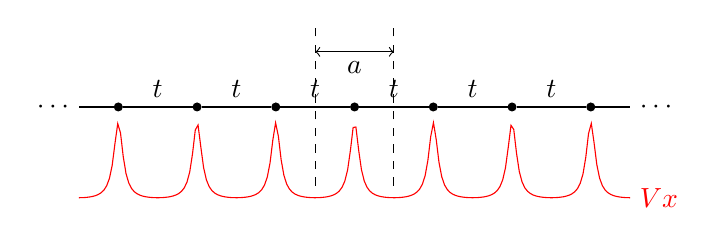
\begin{tikzpicture}
        \foreach \i in {1,...,7}
        {
            \node[draw, fill, circle, inner sep=1pt] (\i) at (\i,0) {};
        }
        \draw[] (1) -- node[above]{$t$} (2);
        \draw[] (2) -- node[above]{$t$} (3);
        \draw[] (3) -- node[above]{$t$} (4);
        \draw[] (4) -- node[above]{$t$} (5);
        \draw[] (5) -- node[above]{$t$} (6);
        \draw[] (6) -- node[above]{$t$} (7);

        \draw[] (1) -- ++(-0.5, 0) node[left]{$\cdots$};
        \draw[] (7) -- ++(+0.5, 0) node[right]{$\cdots$};

        \draw[dashed] (3.5, -1) -- (3.5, 1);
        \draw[dashed] (4.5, -1) -- (4.5, 1);
        \draw[<->] (3.5, +0.7) -- node[below]{$a$} (4.5, +0.7);
        \draw[scale=1.0,domain=0.5:7.5,samples=200,variable=\x,red] plot ({\x},{0.05/((cos(deg(pi*(\x+1/2))))^2 + 0.05) - 1.2}) node[right]{$V\br{x}$};
    \end{tikzpicture}
\end{center}


Now consider an electron moving in this potential. Quantum mechanically we anticipate any electron motion to be due to the effects of quantum tunneling. Specifically, the is expected that if an electron were to tunnel at all, it would be most likely to tunnel to its nearest neighboring atoms with some amplitude $t$. If we let $\ket{n}$ denote the state of an electron localized to the $n$-th atom ($n \in \Z$) at position $na$ in this lattice we can consider two possible ways any electron can tunnel away from $\ket{n}$.

\begin{alignat*}{2}
    \ket{n} &\stackrel{t}{\longrightarrow} \ket{n+1} \quad &&\text{transition to the right} \\
    \ket{n} &\stackrel{t}{\longrightarrow} \ket{n-1} \quad &&\text{transition to the left}
\end{alignat*}

Therefore, one can write the Hamiltonian for this system as follows,
\[ H = -t \sum_{n}\br{\underbrace{\ket{n+1}\bra{n}}_{\longrightarrow} + \underbrace{\ket{n-1}\ket{n}}_{\longleftarrow}} \eq \label{eq:toy_hamiltonian}\]
Where the preceding minus is simply convention. Notice that we are omitting the localized terms in this Hamiltonian because we can take the potential energy to be zero.
\[ \bramidket{n}{H}{n} = \bramidket{n}{V}{n} = 0 \qquad \text{Since $V\br{na} \defined 0$} \]

In order to find the energy eigenstates of the Hamiltonian \cref{eq:toy_hamiltonian} we need to find states $\ket{\psi}$ such that $H \ket{\psi} = E \ket{\psi}$. Evidently, \cref{eq:toy_hamiltonian} is non-diagonal in the $\ket{n}$ basis. Instead consider a different basis indexed by $k$ such that,
\[ \ket{n} = \sum_{k} \ket{k}\braket{k}{n} \eq \label{eq:toy_basis_change}\]
If this new basis represents momentum states, then $\braket{k}{n}$ has a specific form. Motivated by free electrons, $\braket{k}{x} \propto e^{-ikx}$ we map $x$ to the position in the crystal:
\[ x \mapsto na \]
Therefore the coefficients in \cref{eq:toy_basis_change} have similar form,
\[ \braket{k}{n} \propto e^{- ikna} \eq \label{eq:toy_plane_wave}\]
The normalization factor comes from completeness,
\[ \sum_{n} \abs{\braket{n}{k}}^2 = 1 \eq \label{eq:toy_normalization}\]
Heretofore, no restrictions have been made on the range of $n$. Evidently, a real substance will possess finite, albeit many, unit cells (atoms). Let $n \in \Z$ be an integer but equip this model with periodic boundary conditions such that there are $N$ distinct position states representing the number of unit cells. This periodic boundary condition can be written as,
\[ \ket{n} = \ket{n + N} \eq \label{eq:toy_periodic_boundary}\]
Letting $\ga \in \R$ be the normalization coefficient in \cref{eq:toy_plane_wave}, \cref{eq:toy_normalization} becomes,
\[ 1 = \sum_{n=1}^{N} \abs{\ga e^{ikna}}^2 = N \ga^2 \implies \ga = \f{1}{\sqrt{N}}\]
Consequently, \cref{eq:toy_basis_change} can be written as follows,
\[ \ket{n} = \f{1}{\sqrt{N}} \sum_{k} e^{- ikna} \ket{k} \eq \label{eq:toy_fourier_transform} \]
Additionally, the periodic boundary condition of \cref{eq:toy_periodic_boundary} gives,
\[  \ket{n} =\ket{n+N} = \f{1}{\sqrt{N}} \sum_{k} e^{- ik\br{n+N}a} \ket{k} = \f{1}{\sqrt{N}} \sum_{k} e^{- ikna} \ket{k}  \]
Therefore $e^{- ikNa} = 1$ which gives,
\[ k = \f{2\pi m}{Na} \qquad m \in \Z \eq \label{eq:toy_k_discrete}\]
Therefore $k$ must be discrete. Note that this assumption was already made above when we insisted that \cref{eq:toy_basis_change} as a new basis for the same Hilbert space. In fact, \cref{eq:toy_fourier_transform} is simply a Fourier transform that is commonly called an \term{inverse lattice Fourier transform}. Additionally, combining this with dimensionality of $\ket{n}$ gives the following constraint on the values of $k$,
\[ -\f{\pi}{a} \leq k < \f{\pi}{a} \]
Effectively corresponds to demanding that there are $N$ possible distinct values of $k$.
\[ m \in \bc{ \f{-N}{2},  \f{-N+1}{2},\ldots,  \f{N-1}{2}, \f{N}{2} } \]
\[ k \in \bc{\f{2\pi}{Na} \f{-N}{2}, \f{2\pi}{Na} \f{-N+1}{2},\ldots, \f{2\pi}{Na} \f{N-1}{2},\f{2\pi}{Na} \f{N}{2} } \eq \label{eq:discrete_finite_k} \]
In order to substitute \cref{eq:toy_fourier_transform} into \cref{eq:toy_hamiltonian}, first take the dual of \cref{eq:toy_fourier_transform},
\[ \bra{n} = \f{1}{\sqrt{N}} \sum_{k} e^{ikna} \bra{k} \eq \label{eq:dual_toy_fourier_transform} \]
Therefore \cref{eq:toy_hamiltonian} becomes,
\[ H = -t\f{1}{N} \sum_{n}\sum_{k,k'}\bc{\br{e^{-ik\br{n+1}a} \ket{k}}\br{e^{ik'na} \bra{k'}} + \br{e^{-ik\br{n-1}a} \ket{k}}\br{e^{ik'a} \bra{k'}}} \]
\[ H = -t\f{1}{N} \sum_{n}\sum_{k,k'}\bc{e^{-ik\br{n+1}a}e^{ik'na} \ket{k}\bra{k'} + e^{-ik\br{n-1}a}e^{ik'a} \ket{k}\bra{k'}} \eq \label{eq:nearly_toy_diag}\]
By \cref{eq:toy_k_discrete}, $\br{k - k'}$ is an integer multiple of $2 \pi / Na$. Letting that integer be $\mu$ we have the following identity:
\[ \f{1}{N} \sum_{n=1}^{N} e^{i\br{k - k'}na} = \f{1}{N} \sum_{n=1}^{N} e^{i2 \pi \mu n / N} = \de_{\mu} = \de_{k, k'}  \eq \label{eq:crucial_idenity}\]
Therefore \cref{eq:nearly_toy_diag} simplifies greatly,
\[ H = -t \sum_{k,k'} \de_{k,k'} \bc{e^{-ika} \ket{k}\bra{k'} + e^{ika} \ket{k}\bra{k'}} \]
\[ H = -t \sum_{k}\bc{e^{-ika} + e^{ika}} \ket{k}\bra{k} \]
\[ H = -2t\cos\br{ka} \sum_{k}\ket{k}\bra{k} \eq \label{eq:toy_hamiltonian_diag}\]
Therefore \cref{eq:toy_hamiltonian_diag} is the diagonalized form of \cref{eq:toy_hamiltonian}. By diagonalizing the Hamiltonian we were able to determine the energy levels $\vep\br{k}$ of the various states,
\[ \varepsilon\br{k} = - 2 t \cos\br{ka} \eq \label{eq:toy_single_energy_band}\]
The momentum space index $k$ is the wave-vector with $p = \hbar k$ where $p$ is an ordinary linear momentum. Additionally, $t$ acts as a tunneling coefficient that dictates a tunneling \textit{rate} (up to a constant $\hbar$) for the electrons in the solid. Unlike free particles, the momentum $k$ in this toy model is confined to a discrete region.
\[ -\f{\pi}{a} \leq k < \f{\pi}{a} \]
This interval is called the \term{first Brillouin zone}. To highlight this difference, we sometimes refer to $p$ in this model as the \term{crystal momentum} of the electron in state $\ket{k}$.\\

Moreover, the periodic boundary conditions restrict $k$ to take on discrete and finite values pursuant to \cref{eq:discrete_finite_k}.
Note that $L = Na$ is the size of the crystal, $N$ is the number of atoms and $a$ is the interval between two atoms in the solid.\\

The states that diagonalized the Hamiltonian are called \term{Bloch states} and are denoted $\ket{k}$ where is given by the inverse crystal Fourier transform (inverse of \cref{eq:toy_fourier_transform}),
\[ \ket{k} = \f{1}{\sqrt{N}} \sum_{n} \ket{n} e^{i k na} \]
Which is a \term{lattice Fourier transform}. Since \cref{eq:toy_single_energy_band} takes on the form of a cosine with amplitude $2t$ the accessible energy levels are confined to the finite interval,
\[ \varepsilon_{\min} = - 2t \qquad \varepsilon_{\max} = + 2t \]
The interval has a width of $\varepsilon_{\max} - \varepsilon_{\min} = 4t$ and is referred to as the allowed energy \textit{band}.

\begin{center}
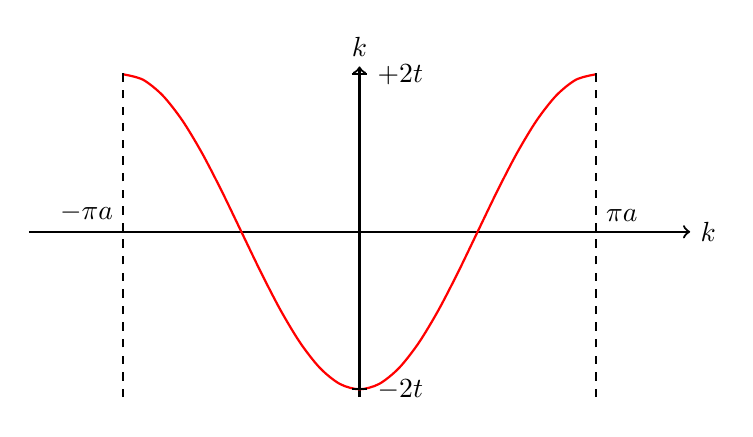
\begin{tikzpicture}
    \pgfmathsetmacro{\axissize}{2.1};
    \pgfmathsetmacro{\plotsize}{3};
    \draw[thick,->] (-2*\axissize,0) -- (+2*\axissize,0) node[right]{$k$};
    \draw[thick,->] (0, -\axissize) -- (0,+\axissize) node[above]{$\vep\br{k}$};
    \draw[thick,scale=1.0,domain=-pi:pi,smooth,variable=\k,red] plot ({\k/pi*\plotsize},{-2*cos(deg(\k))});
    \draw[thick,dashed] (\plotsize, -\axissize) -- node[above right]{$\f{\pi}{a}$} (\plotsize,+\axissize);
    \draw[thick,dashed] (-\plotsize, -\axissize) -- node[above left]{$-\f{\pi}{a}$} (-\plotsize,+\axissize);
    \draw[thick,-] (-0.1,-2) -- (+0.1,-2) node[right]{$-2t$};
    \draw[thick,-] (-0.1,+2) -- (+0.1,+2) node[right]{$+2t$};
\end{tikzpicture}
\end{center}

Given \cref{eq:discrete_finite_k}, there are $N$ distinct Bloch vector states $\ket{k}$. Suppose now that we have $1$ electron per atom (instead of $1$ electron in total). We recall the \term{Pauli principle} which states that only $1$ electron can occupy a given state in a band. If there is one electron per atom and $N$ total atoms, there are $N$ electrons. If we recall the fact that electrons are spin-$1/2$ fermions, each momentum state corresponds to two distinct spin states. Therefore in total there are $2N$ states accessible to the electrons and therefore the band is \textit{half-filled}.
\begin{center}
\begin{tikzpicture}
    \pgfmathsetmacro{\axissize}{4};
    \pgfmathsetmacro{\plotsize}{3};
    \draw[->] (0,0) -- (+\axissize,0) node[right]{$T$};
    \draw[->] (0, 0) -- (0,+\axissize) node[above]{$\rho\br{T}$};
    \draw[scale=1.0,domain=0.25:\plotsize,smooth,variable=\T,red] plot ({\T},{1/\T});
\end{tikzpicture}
\end{center}

Of course, this holds when the electrons in the material are at zero temperature where the electrons occupy all of the lowest possible energy states. For a half-filled energy band, all of the \textit{negative} energy states are filled and the positive energy states are vacant. This separation defines the \term{Fermi energy} for this system which occurs at the interface between filled energy states and unfilled energy states ($\vep\tsb{F} = 0$ in this problem). In order to find the state that corresponds to this upper limit one needs to solve,
\[ \vep\br{k} = \vep\tsb{F} = 0 \implies -2t \cos\br{ka} = 0 \]
Therefore the value of $k$ that solves this equation is,
\[  k = \pm \f{\pi}{2a} = \pm k\tsb{F}\]
Where $k\tsb{F}$ is given a special name: the \term{Fermi wave-vector} (Fermi momentum).
\begin{align*}
    \abs{k} < k\tsb{F} &: \text{filled states}\\
    \abs{k} > k\tsb{F} &: \text{empty states}
\end{align*}
The \term{Fermi surface} defines the surface in momentum space separating the filled states from the unfilled states. Most of the observed properties of metals follow from the existence of the Fermi surface. \\

This concept is so important that it is worth measuring the volume \text{in momentum space} corresponding to the filled states. This is the volume enclosed by the Fermi surface. In this example, the volume in momentum space is characterized by the $2 k\tsb{F}$ interval. Since $k = 2\pi m / Na$, the volume per single $k$-value is $2 \pi / Na$. Letting $n = 1/a$ be the linear density of electrons per unit length, we can compute the total number of electrons:
\[ N =  n N a = 2 \f{2k\tsb{F}}{2 \pi / Na} \]
Which allows one to calculate $k\tsb{F}$ in terms of the electron density $n$,
\[ k\tsb{F} =\f{\pi}{2} n \]
Which makes sense for this model because there is one electron per atom making $n = 1/a$.
This result is called \term{Luttinger's theorem} which states that the volume enclosed by the Fermi surface (sometimes called the Fermi sea) is directly proportional to the electron density. \\

\subsection{Polyacetylene}

In \cref{sec:toy_model} we considered a one dimensional toy model of electrons in a solid. This model is highly idealized and is fair from a description of a real material. It is possible however to modify the model analyzed in \cref{sec:toy_model} to consider the case of the one dimensional polymer called polyacetylene. Polyacetylene consists of weakly-interacting chains of CH units.
\begin{align*}
    \text{C} &: 1s^2 2s^2 2p^2 \qquad \text{4 valence electrons}\\
    \text{H} &: 1s^1
\end{align*}

Electrons found in the inner orbitals of the atoms are tightly bound to their nuclei and therefore only the valence electrons in carbon are free to travel throughout the lattice.

\begin{center}
    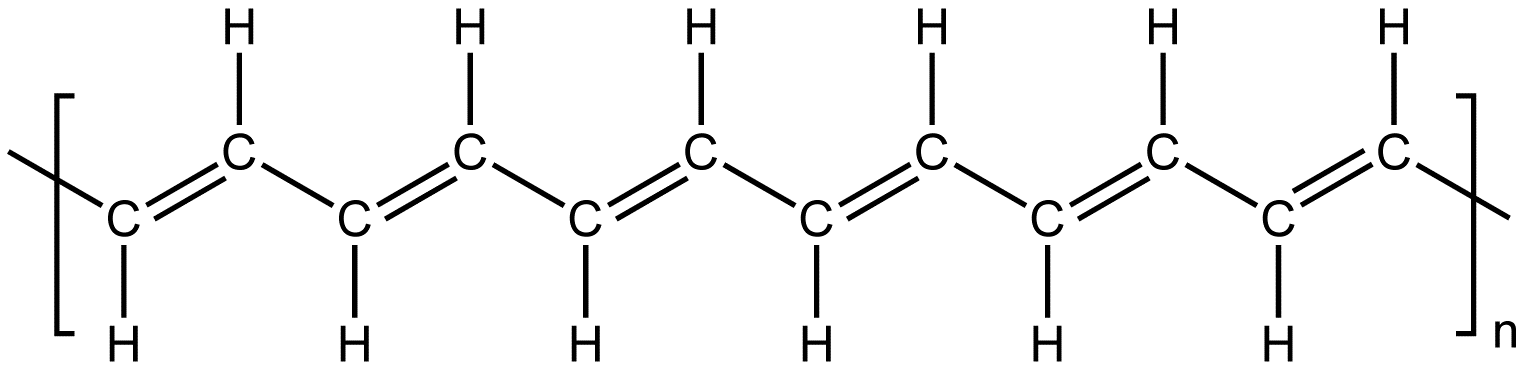
\includegraphics[width=\linewidth]{figures/polyacetylene.png}
\end{center}

Three of the valence electrons are engaged in bonding with neighboring carbon and hydrogen atoms while the $4$-th one is free to move around. As it turns out, the bonds between carbon atoms possess alternating tunneling amplitudes.

\begin{center}
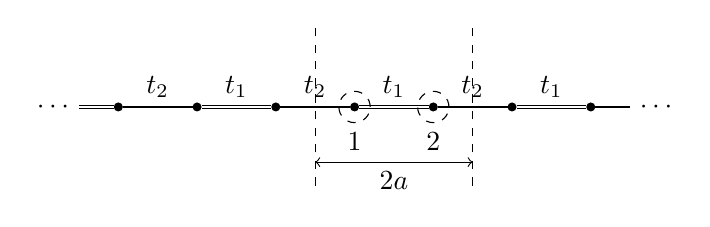
\begin{tikzpicture}
    \foreach \i in {1,...,7}
    {
        \node[draw, fill, circle, inner sep=1pt] (\i) at (\i,0) {};
    }
    \draw[]       (1) -- node[above]{$t_2$} (2);
    \draw[double] (2) -- node[above]{$t_1$} (3);
    \draw[]       (3) -- node[above]{$t_2$} (4);
    \draw[double] (4) -- node[above]{$t_1$} (5);
    \draw[]       (5) -- node[above]{$t_2$} (6);
    \draw[double] (6) -- node[above]{$t_1$} (7);

    \node[dashed, draw, circle, inner sep=4pt, label={below:$1$}] at (4,0) {};
    \node[dashed, draw, circle, inner sep=4pt, label={below:$2$}] at (5,0) {};

    \draw[double] (1) -- ++(-0.5, 0) node[left]{$\cdots$};
    \draw[]       (7) -- ++(+0.5, 0) node[right]{$\cdots$};

    \draw[dashed] (3.5, -1) -- (3.5, 1);
    \draw[dashed] (5.5, -1) -- (5.5, 1);
    \draw[<->] (3.5, -0.7) -- node[below]{$2a$} (5.5, -0.7);
\end{tikzpicture}
\end{center}
In Polyacetylene, the tunneling amplitude between the carbon atoms joined by a double bound is slightly higher $t_1 > t_2$. This is referred to as \term{Peierls instability}. \\

Since this deviation is only slight, let $2\de t = t_1 - t_2$ be a small perturbation such that,
\[ t_1 = t + \de t \qquad t_2 = t - \de t \eq \label{eq:t1t2}\]
Another important difference is that the primitive unit cell has size $2a$ (instead of $a$). This two atom basis can be arranged on a lattice with lattice constant $2a$. This is referred to as a \term{Bravais lattice}. Notationally, we can describe any crystal as,
\[ \text{crystal} = \br{\text{basis}, \text{Bravais lattice}} \]

To describe an electron in this lattice, we need two indices: one to describe the unit cell the electron is in ($n$) and one to describe which atom ($1$ or $2$) the electron is located at within the unit cell. Therefore the Hamiltonian needs to characterize a number of possible transitions,

\begin{alignat*}{2}
    \ket{n, 1} &\stackrel{t_1}{\longrightarrow} \ket{n, 2} \quad &&\text{transition to the right within a unit cell} \\
    \ket{n, 2} &\stackrel{t_1}{\longrightarrow} \ket{n, 1} \quad &&\text{transition to the left within a unit cell} \\
    \ket{n, 1} &\stackrel{t_2}{\longrightarrow} \ket{n-1, 2} \quad &&\text{transition to the left across a unit cell} \\
    \ket{n, 2} &\stackrel{t_2}{\longrightarrow} \ket{n+1, 1} \quad &&\text{transition to the right across a unit cell}
\end{alignat*}

Just as before in \cref{sec:toy_model}, we only consider the tunneling of electrons for nearest neighbors. This will be a recurring motif of this class which is formally called the \term{tight-binding model}.
\[ H = \sum_{n} \bc{ - t_1 \ket{n, 2} \bra{n, 1} - t_2 \ket{n-1, 2} \bra{n, 1} - t_1 \ket{n, 1} \bra{n, 2} - t_2 \ket{n+1, 1} \bra{n, 2}} \eq \label{eq:polyacetylene_tight_binding}\]
Just as before, we need to write $\ket{n, \al}$ in the momentum basis (a new basis for each $\al \in \bc{1,2}$),
\[ \ket{n, \al} = \sum_{k} \ket{k,\al} \braket{k, \al}{n, \al} \eq \label{eq:basis_change}\]
where $\braket{k, \al}{n, \al}$ has a specific form. Motivated by free electrons, $\braket{k}{x} \propto e^{-ikx}$ we map $x$ to the position in the crystal:
\[ x \mapsto n\cdot2a \]
Noting the factor of $2$ because the unit call is twice as long as before. The coefficients in \cref{eq:basis_change} have similar form,
\[ \braket{k, \al}{n, \al} \propto e^{- i2kna} \eq \label{eq:plane_wave}\]
The normalization factor comes from completeness,
\[ \sum_{n} \abs{\braket{n, \al}{k, \al}}^2 = 1 \eq \label{eq:normalization}\]
Analogously to \cref{sec:toy_model}, let $n \in \Z$ be an integer but equip this model with periodic boundary conditions such that there are $N$ distinct positions for the electron for each $\al \in \bc{1,2}$ representing the number of unit cells. It is important to note that here $N$ does not represent the total number of atoms; $N$ is the total number of unit cells (equivalently the total number of distinct $\ket{n, \al}$ states for \textit{fixed} $\al$). Moreover the extra factor of $2$ in the exponential is due to the increases unit cell size.
Therefore the periodic boundary conditions for each $\al$ are,
\[ \ket{n, \al} = \ket{n + N, \al} \eq \label{eq:periodic_boundary}\]
Letting $\ga \in \R$ be the normalization coefficient in \cref{eq:plane_wave}, \cref{eq:normalization} becomes,
\[ 1 = \sum_{n=1}^{N} \abs{\ga e^{i2kna}}^2 = N \ga^2 \implies \ga = \f{1}{\sqrt{N}}\]
Consequently, \cref{eq:basis_change} can be written as follows,
\[ \ket{n, \al} = \f{1}{\sqrt{N}} \sum_{k} e^{- i2kna} \ket{k, \al}  \]
Additionally, the periodic boundary condition of \cref{eq:periodic_boundary} gives,
\[  \ket{n, \al} =\ket{n+N, \al} = \f{1}{\sqrt{N}} \sum_{k} e^{- i2k\br{n+N}a} \ket{k, \al} = \f{1}{\sqrt{N}} \sum_{k} e^{- i2kna} \ket{k, \al}  \]
Therefore $e^{- i2kNa} = 1$ which gives,
\[ k = \f{\pi m}{Na} \qquad m \in \Z \eq \label{eq:k_discrete}\]
Therefore $k$ must be discrete (an assumption made above to write down \cref{eq:basis_change}). Additionally, combining this with dimensionality of $\ket{n, \al}$ gives the following constraint on $k$,
\[ -\f{\pi}{2a} \leq k < \f{\pi}{2a} \]
Note the Brillouin zone for Polyacetylene is half the width of the Brillouin zone for the toy model discussed in \cref{sec:toy_model} (again this is due to the unit cell being twice the size). Thus ensures there are $N$ states of the form $\ket{k, \al}$. \\

Substituting these results into \cref{eq:polyacetylene_tight_binding} gives,
\begin{align*}
\eq \label{eq:H_polyacetylene}
\begin{split}
H
&= - t_1 \f{1}{N} \sum_{n} \sum_{k_1 ,k_2} \ket{k_1, 2}\bra{k_2, 1} e^{-2ik_1na}e^{2ik_2na} \\
&\quad  - t_2 \f{1}{N} \sum_{n} \sum_{k_1 ,k_2} \ket{k_1, 2}\bra{k_2, 1} e^{-2ik_1\br{n-1}a}e^{2ik_2na} \\
&\quad  - t_1 \f{1}{N} \sum_{n} \sum_{k_1 ,k_2} \ket{k_1, 1}\bra{k_2, 2} e^{-2ik_1na}e^{2ik_2na} \\
&\quad  - t_2 \f{1}{N} \sum_{n} \sum_{k_1 ,k_2} \ket{k_1, 1}\bra{k_2, 2} e^{-2ik_1na}e^{2ik_2\br{n-1}a}
\end{split}
\end{align*}
\begin{align*}
    \eq \label{eq:H_energy_difference_ks_diag}
    \begin{split}
    H
    &= \f{1}{N}\sum_{n} \sum_{k_1, k_2} \ket{k_1, 1}\bra{k_2, 2} \bc{-t_1 e^{i2\br{k_2 - k_1}na} - t_2 e^{- i2k_1a}e^{i2\br{k_2 - k_1}na}}+ \cdots\\
    &\cdots + \f{1}{N}\sum_{n} \sum_{k_1, k_2} \ket{k_1, 2}\bra{k_2, 1} \bc{-t_1 e^{i2\br{k_2 - k_1}na} - t_2 e^{+ i2k_1a}e^{i2\br{k_2 - k_1}na}}
    \end{split}
\end{align*}
By \cref{eq:k_discrete}, $\br{k_2 - k_1}$ is an integer multiple of $\pi / Na$. Letting that integer be $\mu$ we have the following identity:
\[ \f{1}{N} \sum_{n=1}^{N} e^{i2\br{k_2 - k_1}na} = \f{1}{N} \sum_{n=1}^{N} e^{i2 \pi \mu n / N} = \de_{\mu} = \de_{k_1, k_2} \]
Therefore \cref{eq:H_energy_difference_ks_diag} simplifies greatly,
\begin{align*}
    \eq \label{eq:H_energy_difference_ks_diag_simp}
    \begin{split}
    H
    &= - t_1 \sum_{k}\bc{\ket{k ,2} \bra{k, 1} + \ket{k, 1}\bra{k,2}} \\
    &\quad - t_2 \sum_{k}\bc{\ket{k ,2} \bra{k, 1}e^{2ika} + \ket{k, 1}\bra{k,2}e^{-2ika}}
    \end{split}
\end{align*}

At this point \cref{eq:H_energy_difference_ks_diag_simp} has been diagonalized with respect to the momentum index $k$ (it is a simple sum over $k$). It is not however diagonalized completely. To diagonalize this Hamiltonian further, we can write $H = \sum_{k} H\br{k}$ where $H\br{k}$ is the summand of \cref{eq:H_energy_difference_ks_diag_simp}. Henceforth, the dependence of $k$ can be omitted from the states $\ket{k, \al}$ for convenience.

\[ H\br{k} = - \br{t_1 + t_2 e^{- i2ka} }\ket{1}\bra{2} - \br{t_1 + t_2 e^{+ i2ka} }\ket{2}\bra{1} \]
Notice that $H\br{k}$ can be written as a $2\times 2$ matrix as follows,
\[ H\br{k} = \kbordermatrix{ & 1 & 2 \\ 1 & 0 & - \br{t_1 + t_2 e^{- i2ka} } \\ 2 & - \br{t_1 + t_2 e^{+ i2ka} } & 0 } \eq \label{eq:H_matrix}\]
Since $H\br{k}$ represents a two level system, we can therefore write $H\br{k}$ as a sum over the three Pauli matrices with the following spin-correspondence (which we refer to as a \term{pseudo-spin}),
\[ \ket{1} = \ket{\uu} \qquad \ket{2} = \ket{\dd} \]
The \term{Pauli matrices} are,
\begin{align*}
\eq \label{eq:pauli_matrices}
\begin{split}
\si_x &= \begin{pmatrix} 0 & 1 \\ 1 & 0 \end{pmatrix} = \ket{1} \bra{2} + \ket{2} \bra{1} \\
\si_y &= \begin{pmatrix} 0 & -i \\ i & 0 \end{pmatrix} = -i\br{\ket{1} \bra{2} - \ket{2} \bra{1}} \\
\si_z &= \begin{pmatrix} 1 & 0 \\ 0 & -1 \end{pmatrix} = \ket{1} \bra{1} - \ket{2} \bra{2}
\end{split}
\end{align*}
Upon close inspection of \cref{eq:H_matrix}, it becomes easy to identity the Pauli's within $H\br{k}$. Explicitly the $t_1$ term is easy,
\[ H\br{k} = \ep \si_z - t_1 \si_x - t_2 \begin{pmatrix} 0 & e^{- i2ka} \\ e^{+ i2ka} & 0 \end{pmatrix}\]
The remaining decomposition follows from $e^{\pm ix} = \cos\br{x} \pm i \sin \br{x}$
\[ H\br{k} = \ep \si_z - t_1 \si_x - t_2 \cos\br{2 k a}\si_x - t_2 \sin\br{2 k a}\si_y \]
Alternatively it is possible to finding  this correspondence by making use of (pseudo-)ladder operators of \cref{eq:pauli_matrices},
\[ \ket{1}\bra{2} = \f{1}{2}\br{\si_x + i \si_y} \qquad \ket{2}\bra{1} = \f{1}{2}\br{\si_x - i \si_y} \]
We therefore define $\ve d \br{k}$ as an \term{effective magnetic field} such that,
\[ \ve d\br{k} = \begin{pmatrix} d_x\br{k} \\ d_y\br{k} \\ d_z\br{k} \end{pmatrix} = \begin{pmatrix} -t_1 - t_2 \cos\br{2 k a} \\ - t_2 \sin\br{2 k a} \\ 0 \end{pmatrix} \eq \label{eq:dk}\]
Therefore $H\br{k} = \ve d\br{k} \cdot \ve \si$. This system is \textit{equivalent} to a spin-1/2 particle in a magnetic field of the form $\ve d\br{k}$. The eigenstates of $H\br{k}$ correspond to $\ba{\ve \si}$ along $\ve d$ or in the opposite direction to $\ve d$.
\[ \vep_{-}\br{k} = -\abs{\ve d \br{k}} \qquad \vep_{+}\br{k} = +\abs{\ve d \br{k}} \]
Using \cref{eq:t1t2},
\begin{align*}
\eq \label{eq:dk_alt}
\begin{split}
d_x \br{k} &= - \br{t + \de t} - \br{t - \de t} \cos\br{2 ka} \\
d_y \br{k} &= - \br{t - \de t} \sin\br{2 ka} \\
d_z \br{k} &= 0
\end{split}
\end{align*}
This is contrasting to the previous model; before we had a \textit{single} energy band pursuant to \cref{eq:toy_single_energy_band}, but here we have \textit{two energy bands}. This result can be generalized to the following observation:
\begin{center}
    \textit{Every atom in the unit cell will give rise to a separate band.}
\end{center}
Explicitly, $\abs{\ve d \br{k}}^2$ can be calculated from \cref{eq:dk_alt},
\[ \abs{\ve d \br{k}}^2 = d_x^2 \br{k} + d_y^2 \br{k} + d_z^2 \br{k} = 4 t^2 \cos^2 \br{ka} + 4 \de t^2 \sin^2 \br{ka} \]
Which makes the two bands have the form,
\[ \vep_{\pm}\br{k} = \pm 2 \sqrt{t^2 \cos^2\br{ka} + \de t^2 \sin^2\br{ka}} \]
Which when plotted is,
\begin{center}
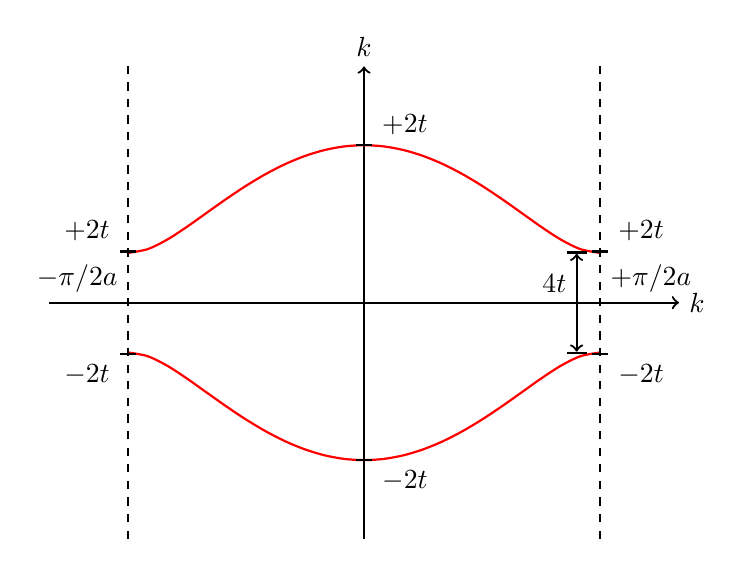
\begin{tikzpicture}
    \pgfmathsetmacro{\axissizev}{3};
    \pgfmathsetmacro{\axissizeh}{4};
    \pgfmathsetmacro{\plotsize}{3};
    \pgfmathsetmacro{\dt}{0.65};
    \draw[thick,->] (-\axissizeh,0) -- (+\axissizeh,0) node[right]{$k$};
    \draw[thick,->] (0, -\axissizev) -- (0,+\axissizev) node[above]{$\vep\br{k}$};
    \draw[thick,scale=1.0,domain=-pi/2:pi/2,smooth,variable=\k,red] plot ({2 *\k/pi*\plotsize},{-2*sqrt(cos(deg(\k))^2 + 0.1*sin(deg(\k))^2)});
    \draw[thick,scale=1.0,domain=-pi/2:pi/2,smooth,variable=\k,red] plot ({2 *\k/pi*\plotsize},{2*sqrt(cos(deg(\k))^2 + 0.1*sin(deg(\k))^2)});
    \draw[thick,dashed] (\plotsize, -\axissizev) -- node[above right]{$+{\pi}/{2a}$} (\plotsize,+\axissizev);
    \draw[thick,dashed] (-\plotsize, -\axissizev) -- node[above left]{$-{\pi}/{2a}$} (-\plotsize,+\axissizev);
    \draw[thick,] (-0.1,-2) -- (+0.1,-2) node[below right]{$-2t$};
    \draw[thick,] (-0.1,+2) -- (+0.1,+2) node[above right]{$+2t$};
    \draw[thick,] (\plotsize-0.1, \dt) -- (\plotsize+0.1, \dt) node[above right]{$+2\de t$};
    \draw[thick,] (\plotsize-0.1, -\dt) -- (\plotsize+0.1, -\dt) node[below right]{$-2\de t$};
    \draw[thick,] (-\plotsize+0.1, \dt) -- (-\plotsize-0.1, \dt) node[above left]{$+2\de t$};
    \draw[thick,] (-\plotsize+0.1, -\dt) -- (-\plotsize-0.1, -\dt) node[below left]{$-2\de t$};
    \draw[thick,|<->|] (\plotsize-0.3, \dt) -- node[above left]{$4 \de t$} (\plotsize-0.3, -\dt);
\end{tikzpicture}
\end{center}

Notice that the first Brillouin zone is $\f{\pi}{2a} \leq k \leq \f{\pi}{2a}$ is \textit{smaller} than it was previously. In this model, there is one electron per atom and thus two electrons per unit cell. Therefore there are $2N$ electrons. Accounting for spin degeneracies, there are $2N$ accessible states per energy band. At zero temperature, the entire lower band is filled and the upper band is empty. This makes polyacetylene an \term{insulator} because it requires an energy of at least $4 \de t$ in order to transition an electron across the Fermi surface. \\

In the limit of the $\de t \to 0$ one should expect to recover \cref{eq:toy_single_energy_band} from \cref{sec:toy_model},
\[ \lim_{\de t \to 0}\vep_{\pm}\br{k} = \pm 2 \lim_{\de t \to 0}\sqrt{t^2 \cos^2\br{ka} + \de t^2 \sin^2\br{ka}} = \pm 2 t \cos\br{ka}  \]
As expected. Notice however the plot of $\vep\br{k}$ when $\de t = 0$ differs from the one depicted in \cref{sec:toy_model},
\begin{center}
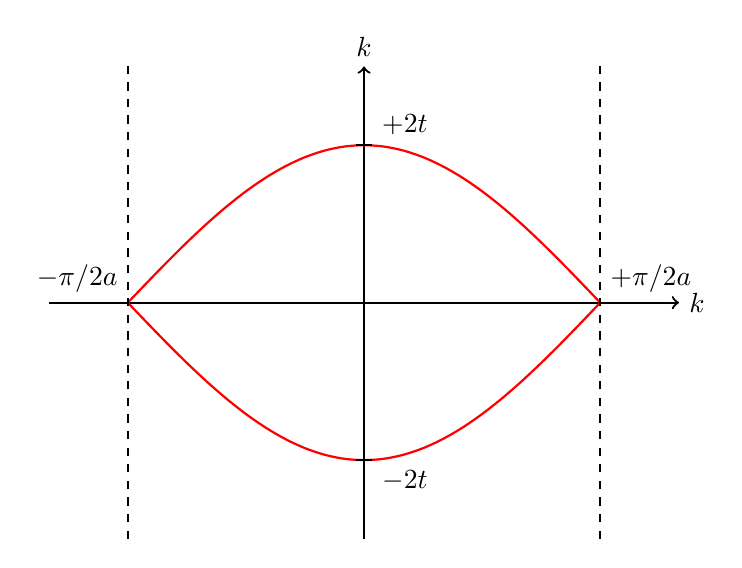
\begin{tikzpicture}
    \pgfmathsetmacro{\axissizev}{3};
    \pgfmathsetmacro{\axissizeh}{4};
    \pgfmathsetmacro{\plotsize}{3};
    \pgfmathsetmacro{\dt}{0.65};
    \draw[thick,->] (-\axissizeh,0) -- (+\axissizeh,0) node[right]{$k$};
    \draw[thick,->] (0, -\axissizev) -- (0,+\axissizev) node[above]{$\vep\br{k}$};
    \draw[thick,scale=1.0,domain=-pi/2:pi/2,smooth,variable=\k,red] plot ({2 *\k/pi*\plotsize},{-2*sqrt(cos(deg(\k))^2)});
    \draw[thick,scale=1.0,domain=-pi/2:pi/2,smooth,variable=\k,red] plot ({2 *\k/pi*\plotsize},{2*sqrt(cos(deg(\k))^2)});
    \draw[thick,dashed] (\plotsize, -\axissizev) -- node[above right]{$+{\pi}/{2a}$} (\plotsize,+\axissizev);
    \draw[thick,dashed] (-\plotsize, -\axissizev) -- node[above left]{$-{\pi}/{2a}$} (-\plotsize,+\axissizev);
    \draw[thick,] (-0.1,-2) -- (+0.1,-2) node[below right]{$-2t$};
    \draw[thick,] (-0.1,+2) -- (+0.1,+2) node[above right]{$+2t$};
\end{tikzpicture}
\end{center}
The resolution between these two plots is to notice that in the polyacetylene model, the unit cell had with $2a$ instead of $a$. Therefore in momentum space, the plotted values for $k$ are bounded by $- \pi / 2a \leq k \leq \pi / 2a$ instead of $- \pi / a \leq k \leq \pi / a$. If one were to unravel the upper band into regions where $\abs{k} > \pi / 2a$ one would recover the initial model. \\

Heretofore, we have assumed that $\de t > 0$. If however we consider $\de t< 0$, then we transition from $t_1 > t_2$ to $t_2 > t_1$ pursuant to \cref{eq:t1t2}. And our diagram is adjusted

\begin{center}
    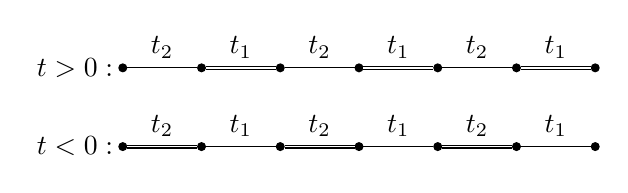
\begin{tikzpicture}
        \foreach \i in {1,...,7}
        {
            \node[draw, fill, circle, inner sep=1pt] (n\i) at (\i,0) {};
            \node[draw, fill, circle, inner sep=1pt] (p\i) at (\i,1) {};
        }
        \draw[]       (p1) -- node[above]{$t_2$} (p2);
        \draw[double] (p2) -- node[above]{$t_1$} (p3);
        \draw[]       (p3) -- node[above]{$t_2$} (p4);
        \draw[double] (p4) -- node[above]{$t_1$} (p5);
        \draw[]       (p5) -- node[above]{$t_2$} (p6);
        \draw[double] (p6) -- node[above]{$t_1$} (p7);
        \draw (p1) node[left]{$\de t > 0 : $};

        \draw[double] (n1) -- node[above]{$t_2$} (n2);
        \draw[]       (n2) -- node[above]{$t_1$} (n3);
        \draw[double] (n3) -- node[above]{$t_2$} (n4);
        \draw[]       (n4) -- node[above]{$t_1$} (n5);
        \draw[double] (n5) -- node[above]{$t_2$} (n6);
        \draw[]       (n6) -- node[above]{$t_1$} (n7);
        \draw (n1) node[left]{$\de t < 0 : $};
    \end{tikzpicture}
\end{center}

Therefore, the ground state of polyacetylene is doubly degenerate, corresponding to the two signs of $\de t$. As it turns out, this difference in sign is related to topological properties in momentum space. Upon examination of \cref{eq:dk} once can notice how $\ve d$ depends on $\de t$. How does $\ve d\br{k}$ change as $k$ goes from $- \pi / 2a$ to $\pi  2a$?
\begin{align*}
\begin{split}
d_x \br{k} &= - \br{t + \de t} - \br{t - \de t} \cos\br{2 ka} \\
d_y \br{k} &= - \br{t - \de t} \sin\br{2 ka}
\end{split}
\end{align*}
Checking specific points,
\begin{align*}
d_x \br{\pm\f{\pi}{2a}} &= - \br{t + \de t} + \br{t - \de t} = - 2 \de t\\
d_y \br{\pm\f{\pi}{2a}} &= 0 \\
d_x \br{0} &= - \br{t + \de t} - \br{t - \de t} = 2 t\\
d_y \br{0} &= 0
\end{align*}
Plotted the case of $\de t >0$ in $d_y, d_x$ space,
\begin{center}
\begin{tikzpicture}
    \pgfmathsetmacro{\axissize}{3};
    \pgfmathsetmacro{\t}{1};
    \pgfmathsetmacro{\dt}{0.1};
    \pgfmathsetmacro{\tick}{0.1};
    \draw[thick,->] (-\axissize,0) -- (+\axissize,0) node[right]{$d_x$};
    \draw[thick,->] (0, -\axissize) -- (0,+\axissize) node[above]{$d_y$};
    \draw[thick,scale=1.0,domain=-pi/2:pi/2,smooth,variable=\k,red] plot ({- (\t + \dt) - (\t - \dt)*cos(deg(2*\k))},{- (\t - \dt)*sin(deg(2*\k))});
    \draw[thick,] (-2*\t, -\tick) -- (-2*\t, \tick) node[above left]{$-2t$};
    \draw[thick,] (-2*\dt, -\tick) -- (-2*\dt, \tick) node[above left]{$-2\de t$};
    \draw[thick,] (- 2, 2) node[]{$\de t > 0$};
\end{tikzpicture}
\end{center}
It can be seen that when $\de t > 0$, the curve in $d_x, d_y$ does not enclose the origin $\ve d = 0$. Recalling that $\vep_{\pm}\br{k} = \pm \abs{\ve d \br{k}}$, as long as $\ve d\br{k} \neq 0$, there exists a energy gap between the two bands $\vep_{+}$ and $\vep_{-}$. Therefore for $\de t > 0$ polyacetylene is an ordinary insulator. However, in the case where $\de t < 0$,
\begin{center}
\begin{tikzpicture}
    \pgfmathsetmacro{\axissize}{3};
    \pgfmathsetmacro{\t}{1};
    \pgfmathsetmacro{\dt}{-0.1};
    \pgfmathsetmacro{\tick}{0.1};
    \draw[thick,->] (-\axissize,0) -- (+\axissize,0) node[right]{$d_x$};
    \draw[thick,->] (0, -\axissize) -- (0,+\axissize) node[above]{$d_y$};
    \draw[thick,scale=1.0,domain=-pi/2:pi/2,smooth,variable=\k,red] plot ({- (\t + \dt) - (\t - \dt)*cos(deg(2*\k))},{- (\t - \dt)*sin(deg(2*\k))});
    \draw[thick,] (-2*\t, -\tick) -- (-2*\t, \tick) node[above left]{$-2t$};
    \draw[thick,] (-2*\dt, -\tick) -- (-2*\dt, \tick) node[above left]{$-2\de t$};
    \draw[thick,] (- 2, 2) node[]{$\de t < 0$};
\end{tikzpicture}
\end{center}
It can be seen that the origin $\abs{\ve d} = 0$ is enclosed. This \textit{topological} difference is what leads us to call the $\de t < 0$ case as a \term{topological insulator} as apposed to an \term{ordinary insulator}. \\

Effectively, there is no possible way to continuously deform the Hamiltonian (i.e. changing $\de t$) without merging the two energy bands; the transition from $\de t > 0$ to $\de t < 0$ permits the band gap to close temporarily. \\

\newcommand{\ppp}[2]{
% \de t
% \ep
\begin{tikzpicture}[scale=0.6]
    \pgfmathsetmacro{\axissize}{4};
    \pgfmathsetmacro{\plotsize}{3};
    \pgfmathsetmacro{\labels}{0.6};
    \pgfmathsetmacro{\dt}{#1};
    \pgfmathsetmacro{\sep}{#2};
    \pgfmathsetmacro{\vs}{1/2};
    \draw[->] (-\axissize,0) -- (+\axissize,0) node[right]{$k a$};
    \draw[->] (0, -\axissize) -- (0,+\axissize) node[above]{${\vep\br{k}}/{t}$};
    \draw (0, \axissize - 1*\labels) node[right]{${\de t}/{t} = \dt$};
    \draw (0, \axissize - 2*\labels) node[right]{${\ep}/{t} = \sep$};
    \draw[thick, scale=1.0,domain=-pi/2:pi/2,variable=\x, red] plot ({\x*\plotsize/(pi/2)},{+\vs*((\sep)^2 + 4*(1)^2*(cos(deg(\x)))^2 + 4*(\dt)^2*(sin(deg(\x)))^2)^(1/2)});
    \draw[thick, scale=1.0,domain=-pi/2:pi/2,variable=\x, red] plot ({\x*\plotsize/(pi/2)},{-\vs*((\sep)^2 + 4*(1)^2*(cos(deg(\x)))^2 + 4*(\dt)^2*(sin(deg(\x)))^2)^(1/2)});
    \draw[dashed] (+\plotsize, -\axissize) node[right]{$+\f{\pi}{2}$} -- (+\plotsize,+\axissize);
    \draw[dashed] (-\plotsize, -\axissize) node[right]{$-\f{\pi}{2}$} -- (-\plotsize,+\axissize);
    % \draw[] (-0.1,-2) -- (+0.1,-2) node[right]{$-2t$};
    % \draw[] (-0.1,2) -- (+0.1,2) node[right]{$2t$};
\end{tikzpicture}
}
\ppp{0.5}{0}
\ppp{0}{0}
\ppp{-0.5}{0}


An observable feature of topological insulators becomes evident for the edge states at zero energy (i.e. in the middle of a band gap). In this case of polyacetylene, these states that are closest to the band gap are those that live on the edge of the Brillouin zone where $\abs{k - \pi / 2a}$ is small. In order to explore the physics of these regions, define $\de k$ such that,
\[ k = \f{\pi}{2a} + \de k \]
Where $\de k$ is small. In this case, the Hamiltonian $H\br{k} = \ve d \br{k} \cdot \ve \si$ can be expanded out explicitly,
\begin{align*}
    d_x\br{k}
    &= d_x\br{\f{\pi}{2a} + \de k} \\
    &= - \br{t + \de t} - \br{t - \de t} \cos \br{\pi + 2 \de k a} \\
    &= - \br{t + \de t} + \br{t - \de t} \cos \br{2 \de k a} \\
    &= - \br{t + \de t} + \br{t - \de t} + \s O \br{\br{\de k}^2} \\
    &\simeq - 2 \de t
\end{align*}
Similarly for $d_y$,
\begin{align*}
    d_y\br{k}
    &= d_y\br{\f{\pi}{2a} + \de k} \\
    &= - \br{t - \de t} \sin \br{\pi + 2 \de k a} \\
    &= \br{t - \de t} \sin \br{2 \de k a} \\
    &= \br{t - \de t} 2 \de k a + \s O \br{\br{\de k}^3} \\
    &\simeq 2 t \de k a
\end{align*}
Therefore,
\[ H\br{\de k} = - 2 \de t \si_x + 2 t a \de k \si_y \]
In order to draw familiarity with systems that have been studied previously, let use rename a number of terms,
\[ 2 \de t = m \qquad 2 t a = \hbar v_F\]
Where $m$ has units of energy and $v_F$ has units of velocity. The Hamiltonian can now be written as,
\[ H = - m \si_x + \hbar v_F \de k \si_y \]
Since $\hbar \de k$ has units of momentum, we simply label it $p$. Then the Hamiltonian can be written as,
\[ H = v_F p \si_y - m \si_x \]
Which is identical to the Dirac equation (1D) for a \textit{relativistic} particle of \textit{mass} $m$ and velocity $v_F$ in place of the speed of light $c$. These velocity $v_F$ is called the \term{Fermi velocity}.

\[ \vep_{\pm}\br{p} = \pm \sqrt{v_F^2 p^2 + m^2} \]

Consider the interface between $2$ polyacetylene samples $\de t > 0$ and $\de t < 0$. In the position basis $p \to - i \hbar \di_x$ we can write our Dirac Hamiltonian as,
\[ H = - i \hbar v_F \si_y \di_x - m\br{x} \si_x \]
Where $m$ has an $x$ dependence.

\[  H \psi = E \psi \]
With $E = 0$ localized near $x = 0$.
\[ \bs{- i \hbar v_F \si_y \di_x - m\br{x} \si_x} \psi\br{x} = 0 \]
Therefore we should look for a solution of the form,
\[ \psi\br{x} = e^{f\br{x}} \si_y \ket{z} \]
Where $\ket{z}$ is written in $\si_z$ basis,
\[ \ket{z} = z_{\uu} \ket{\uu} + z_{\dd} \ket{\dd} \]
Using $\si_y^2 = \ident$ and $\si_x \si_y = i \si_z$ multiply by both sides by $\si_y$,
\[ \bs{-i \hbar v_F \der{f}{x} + i m\br{x} \si_z} e^{f\br{x}}\ket{z} = 0 \]
Dropping the exponential $e^{f\br{x}}$,
\[ \bs{-i \hbar v_F \der{f}{x} + i m\br{x} \si_z} \ket{z} = 0 \]
Adjusting the constant coefficients,
\[ \bs{\der{f}{x} - \f{m\br{x}}{\hbar v_F} \si_z} \ket{z} = 0 \eq \label{eq:mass_varying_eqn}\]
Recalling that,
\[ \si_{z}\ket{\uu} = + \ket{\uu} \qquad \si_{z}\ket{\dd} = - \ket{\dd} \]
Assume $\ket{z} = \ket{\uu}$,
\[ \bs{\der{f}{x} + \f{m\br{x}}{\hbar v_F}} \ket{\uu} = 0 \]
Therefore,
\[ \der{f}{x} = - \f{m\br{x}}{\hbar v_F} \]
Can be solved using,
\[ f\br{x} = - \f{1}{\hbar v_F} \intl_{0}^{x} \dif x' m\br{x'} \]
Where $m\br{0} = 0$. Altogether, the solution $\psi{x}$ can be written,
\[ \psi\br{x} = e^{- \f{1}{\hbar v_F} \int_{0}^{x} \dif x' m\br{x'}} \si_y \ket{\uu} \]
Since $\si_y \ket{\uu} = i \ket{\dd}$,
\[ \psi\br{x} = ie^{- \f{1}{\hbar v_F} \int_{0}^{x} \dif x' m\br{x'}}\ket{\dd} \]
Of course an analogous solution exists for $\ket{z} = \ket{\dd}$.
\begin{center}
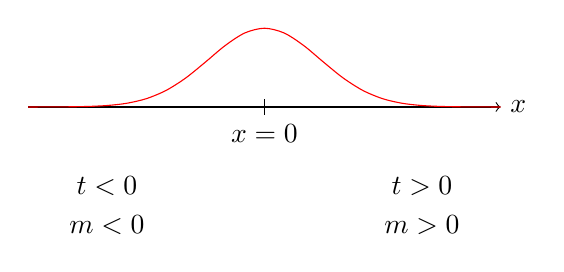
\begin{tikzpicture}
    \draw[->] (-3, 0) -- (3, 0) node[right]{$x$};
    \draw (0, -0.1) node[below]{$x = 0$} -- (0, 0.1);
    \draw (-2, -1) node[]{$\de t < 0$};
    \draw (-2, -1.5) node[]{$m < 0$};
    \draw (2, -1) node[]{$\de t > 0$};
    \draw (2, -1.5) node[]{$m > 0$};
    \draw[scale=1.0,domain=-3:3,smooth,variable=\x,red] plot ({\x},{exp(-\x*\x)});
\end{tikzpicture}
\end{center}

\subsection{Higher Dimensions}

A crystal is an infinite, periodic array of identical groups of atoms,
\[ \text{crystal} = \br{\text{basis}, \text{Bravais lattice}} \]

\begin{center}
    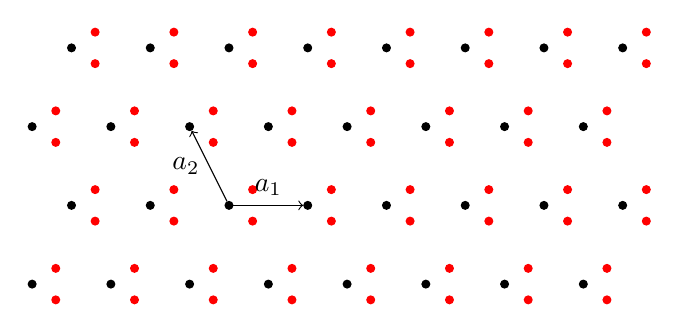
\begin{tikzpicture}
        \foreach \i in {1,...,8}
        {
            \foreach \j in {1,...,4}
            {
                \node[draw, fill, circle, inner sep=1pt] (\i\j) at ({\i+0.5*iseven(\j)},\j) {};
                \node[draw, fill, red, circle, inner sep=1pt] (a\i\j) at ({\i+0.5*iseven(\j)+0.3},\j-0.2) {};
                \node[draw, fill, red, circle, inner sep=1pt] (b\i\j) at ({\i+0.5*iseven(\j)+0.3},\j+0.2) {};
            }
        }
        \draw[->] (32) -- node[left]{$\ve a_2$} (33);
        \draw[->] (32) -- node[above]{$\ve a_1$} (42);
    \end{tikzpicture}
\end{center}

A \term{Bravais lattice} is all points in $\R^{n}$ ($\R^{1}, \R^{2}, \R^{3}$, etc.) such that,
\[ \ve R = n_1 \ve a_1 + n_2 \ve a_2 + n_3 \ve a_3 \eq \label{eq:R_lattice} \]
Where $\ve a_1, \ve a_2, \ve a_3$ are the primitive translation vectors of the Bravais lattice. Moreover the coefficients $n_1, n_2, n_3$ are integers,
\[ n_1, n_2, n_3 = 0, \pm 1, \pm 2, \pm 3, \ldots \]
Typically, the choice for $\ve a_i$ is not unique. However, the best choice for the primitive transition vectors is typically the one that exhibits the most symmetry. \\

The \term{primitive unit cell} is the parallelepiped defined by the primitive translation vectors. A primitive unit cell is also not unique. A special type of unit cell, usually the most convenient, is the \term{Wigner-Seitz unit cell}. A Wigner-Seitz unit cell is the region of space about a Bravais lattice point that are closer to this point than to any other Bravais lattice point. As an example, the first Brillouin zone is the Wigner-Seitz cell in reciprocal (momentum) space. Analogously to \cref{eq:R_lattice} which indexes lattice points in position space, we define the \term{reciprocal lattice} and all points in momentum space $\ve G$ such that,
\[ \ve G = m_1 \ve b_1 + m_2 \ve b_2 + m_3 \ve b_3\]
Provided that we have the following correspondence between $\ve R$ and $\ve G$,
\[ e^{i \ve G \cdot \ve G} = 1 \]
This is equivalent to the following,
\[ \ve b_{i} \cdot \ve a_{j} = 2 \pi \de_{ij} \qquad \forall i,j \]

\subsection{Electronic Structure for Square Lattice}

The square lattice in 2 dimensions has two primitive basis vectors $\ve a_{1}, \ve a_{2}$,
\begin{center}
    \begin{tikzpicture}
        \foreach \i in {1,...,8}
        {
            \foreach \j in {1,...,4}
            {
                \node[draw, fill, circle, inner sep=1pt] (\i\j) at (\i,\j) {};
            }
        }
        \draw[->] (32) -- node[left]{$\ve a_2$} (33);
        \draw[->] (32) -- node[above]{$\ve a_1$} (42);
    \end{tikzpicture}
\end{center}
Using Cartesian coordinates,
\[ \ve a_1 = a \hat x \qquad \ve a_2 = a \hat y \]
The reciprocal lattice has the following form,
\[ \ve b_1 = \f{2 \pi }{a}\hat x \qquad \ve b_2 = \f{2 \pi}{a} \hat y \]
The Hamiltonian for this system in the nearest neighbor approximation can be written as the sum over all possible transitions with tunneling coefficient $t$.
\[ H = - t \sum_{\ve R, \ve a} \br{\ket{\ve R + \ve a} \bra{\ve R} + \ket{\ve R} \bra{\ve R + \ve a}} \eq \label{eq:nearest_neighbor_square_lattice} \]
Where $\ve a \in \bc{\ve a_1, \ve a_2}$. Notice that we only need to sum over terms of the form involving $\ve R + \ve a$ and not $\ve R - \ve a$. If we were to include those terms, we would double-count all each of the possible transitions. In order to diagonalize \cref{eq:nearest_neighbor_square_lattice} we use the familiar Fourier transform but here we apply it as a vector change of coordinates,
\[\ket{\ve R} = \sum_{\ve R} \ket{\ve k} \braket{\ve k}{\ve R} \]
Where $\braket{\ve k}{\ve R}$ is normalized in the usual fashion,
\[ \braket{\ve k}{\ve R} = \f{1}{\sqrt{N}} e^{i \ve k \cdot \ve R} \]
Therefore,
\[\ket{\ve R} = \f{1}{\sqrt{N}} \sum_{\ve R} \ket{\ve k}  e^{i \ve k \cdot \ve R} \]
In the reciprocal lattice, $\ve k$ can be written as,
\[ \ve k = k_1 \ve b_1 + k_2 \ve b_2 \]
Where $k_{1}$ and $k_{2}$ are bounded,
\[ -\f12 \leq k_{1}, k_{2} < \f12 \]
Therefore,
\[ \ve k \cdot \ve R = \br{k_1 \ve b_1 + k_2 \ve b_2} \cdot \br{n_1 \ve a_1 + n_2 \ve a_2} \]
\[ \ve k \cdot \ve R = 2 \pi \br{k_1 n_1 + k_2 n_2} \]
Using the $\ket{\ve k}$ basis, \cref{eq:nearest_neighbor_square_lattice} becomes,
\[ H = - t \sum_{\ve R, \ve a} \sum_{\ve k, \ve k'} \br{\ket{\ve k}\bra{\ve k'} e^{-i \ve k \cdot \br{\ve R + \ve a}} e^{i \ve k' \cdot \ve R} + \ket{\ve k}\bra{\ve k'} e^{-i \ve k \cdot \ve R} e^{i \ve k' \cdot \br{\ve R + \ve a}}} \eq \label{eq:nearest_neighbor_square_lattice_momentum} \]
Using a multi-dimensional version of \cref{eq:crucial_idenity},
\[ \f{1}{N} \sum_{\ve R} e^{- i \br{\ve k - \ve k'} \cdot \ve R} = \de_{\ve k, \ve k'} \]
Therefore \cref{eq:nearest_neighbor_square_lattice} becomes,
\[ H = - t \sum_{\ve k, \ve a} \ket{\ve k} \bra{\ve k} \br{e^{- i\ve k \cdot \ve a} + e^{i\ve k \cdot \ve a}} \]
Recognize a cosine term,
\[ H = - 2t \sum_{\ve k, \ve a} \ket{\ve k} \bra{\ve k} \cos \br{\ve k \cdot \ve a} \]
The energy levels (as indexed by $\ve k$) can now be read off easily,
\[ \vep \br{\ve k} = -2 t \sum_{\ve a} \cos \br{\ve k \cdot \ve a} = - 2t \bs{ \cos \br{ ak_x} + \cos \br{ ak_y}} \]
Clearly, $\vep\br{\ve k}$ has minimum when $k_x = k_y = 0$. Therefore,
\[ \min\bc{\vep\br{\ve k}} = \vep_{\min} = - 4 t \]
Likewise at the Brillouin zone corners,
\[ \max\bc{\vep\br{\ve k}} = \vep_{\max} = 4 t \]
\begin{center}
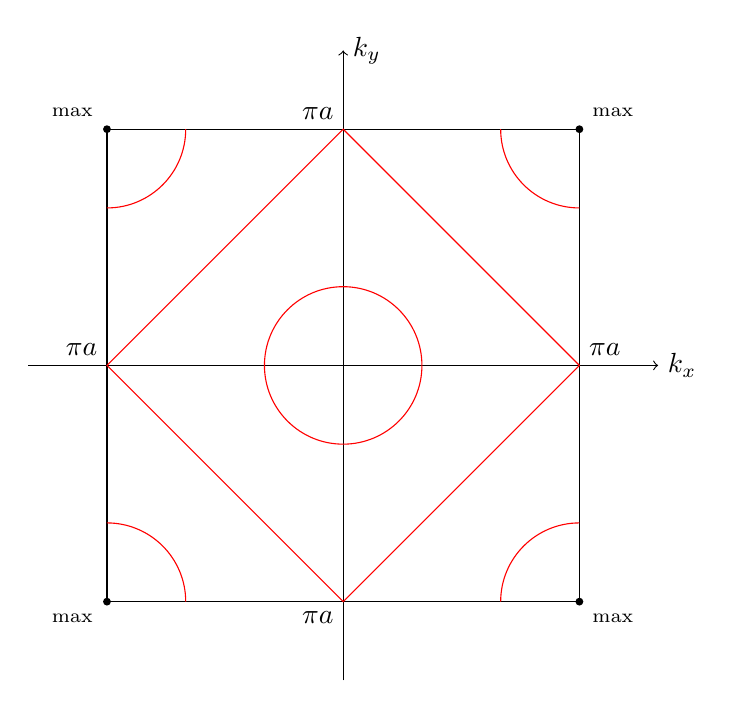
\begin{tikzpicture}
    \pgfmathsetmacro{\plot}{4};
    \pgfmathsetmacro{\edge}{3};
    \pgfmathsetmacro{\oarc}{1};
    \draw[->] (-\plot, 0) -- (\plot, 0) node[right]{$k_x$};
    \draw[->] (0, -\plot) -- (0, \plot) node[right]{$k_y$};
    \draw (+\edge, +\edge) -- (+\edge, -\edge);
    \draw (+\edge, -\edge) -- (-\edge, -\edge);
    \draw (-\edge, +\edge) -- (+\edge, +\edge);
    \draw (-\edge, -\edge) -- (-\edge, +\edge);
    \draw (+\edge, 0) node[above right]{$\f{\pi}{a}$};
    \draw (0, +\edge) node[above left]{$\f{\pi}{a}$};
    \draw (-\edge, 0) node[above left]{$\f{\pi}{a}$};
    \draw (0, -\edge) node[below left]{$\f{\pi}{a}$};
    \draw (+\edge, +\edge) node[circle, inner sep=1pt, fill=black, label={above right:$\vep_{\max}$}]{};
    \draw (-\edge, +\edge) node[circle, inner sep=1pt, fill=black, label={above left:$\vep_{\max}$}]{};
    \draw (+\edge, -\edge) node[circle, inner sep=1pt, fill=black, label={below right:$\vep_{\max}$}]{};
    \draw (-\edge, -\edge) node[circle, inner sep=1pt, fill=black, label={below left:$\vep_{\max}$}]{};
    \draw[red] (+\edge, 0) -- (0, +\edge) -- (-\edge, 0) -- (0, -\edge) -- cycle;
    \draw[red] (0,0) circle (\edge/3);
    \draw[red] (+\edge-\oarc, +\edge) arc (180:270:\oarc);
    \draw[red] (-\edge, +\edge-\oarc) arc (270:360:\oarc);
    \draw[red] (+\edge-\oarc, -\edge) arc (180:90:\oarc);
    \draw[red] (-\edge, -\edge+\oarc) arc (90:0:\oarc);
\end{tikzpicture}
\end{center}
Expanding $\ve k$ near the minimum,
\[ \vep\br{\ve k} \simeq -4t + t a^2 \br{k_x^2 + k_y^2} = -4t + ta^2 k^2 \eq \label{eq:minimum_k}\]
Notice that this looks like the dispersion of a free electron.
Recall that for a free electron,
\[ \vep \br{\ve k} = \f{\hbar^2 k^2}{2 m} \]
Therefore we can define an effective mass $m^{*}$ as follows,
\[ \vep \br{\ve k} - \vep_{\min} = ta^2 k^2 = \f{\hbar^2 k^2}{2 m^{*}} \]
Where the effective mass is,
\[ m^{*} = \f{\hbar^2}{2 t a^2} \]
In conclusion, electrons near the minimum energy level $\vep_{\min}$ behave like free particles with effective mass $m^{*}$. \\

The Fermi surface in this model can be calculated by setting $\vep \br{\ve k} = \vep\tsb{F}$,
\[ \vep\br{\ve k} = - 4t + \f{\hbar^2 k^2}{2 m^{*}} = \vep\tsb{F}\]
Therefore,
\[ \f{\hbar^2 k^2}{2 m^{*}} = \vep\tsb{F} - \vep_{\min} \]
Defines the equation of a circle in $k_x, k_y$ space with radius,
\[ k_{F} = \sqrt{\f{2m^{*}}{\hbar^2} \br{\vep\tsb{F} - \vep_{\min}}} \]
Recall from \cref{eq:minimum_k} that this equation only defines the Fermi surface near the minimum energy level. In general,
\[ \vep \br{\ve k} = - 2t \br{\cos \br{k_x a} + \cos \br{k_y a}} \]
For a half-filled band, $\vep\tsb{F} = 0$, the Fermi surface is depicted above.

The dispersion relation is,
\begin{center}
    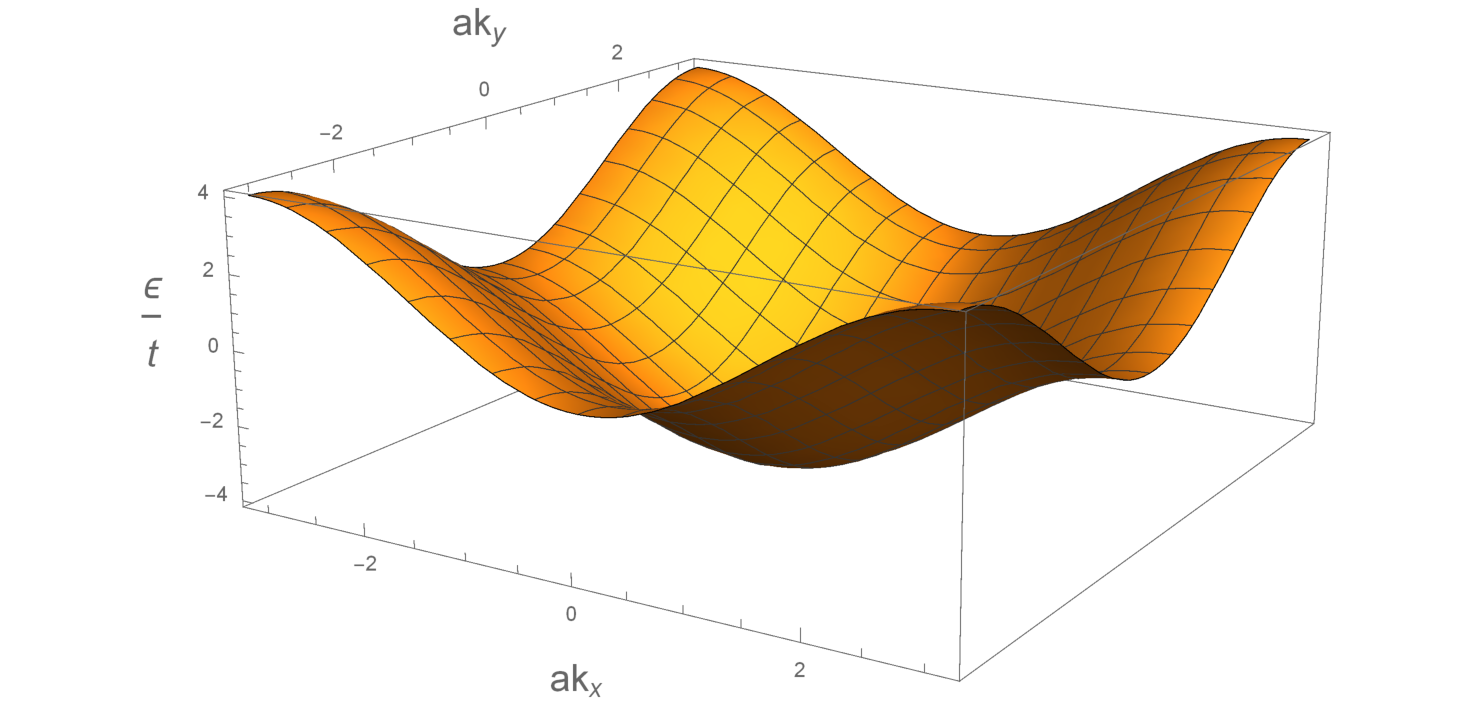
\includegraphics[width=0.9\textwidth]{figures/square_3d_bz.pdf}
    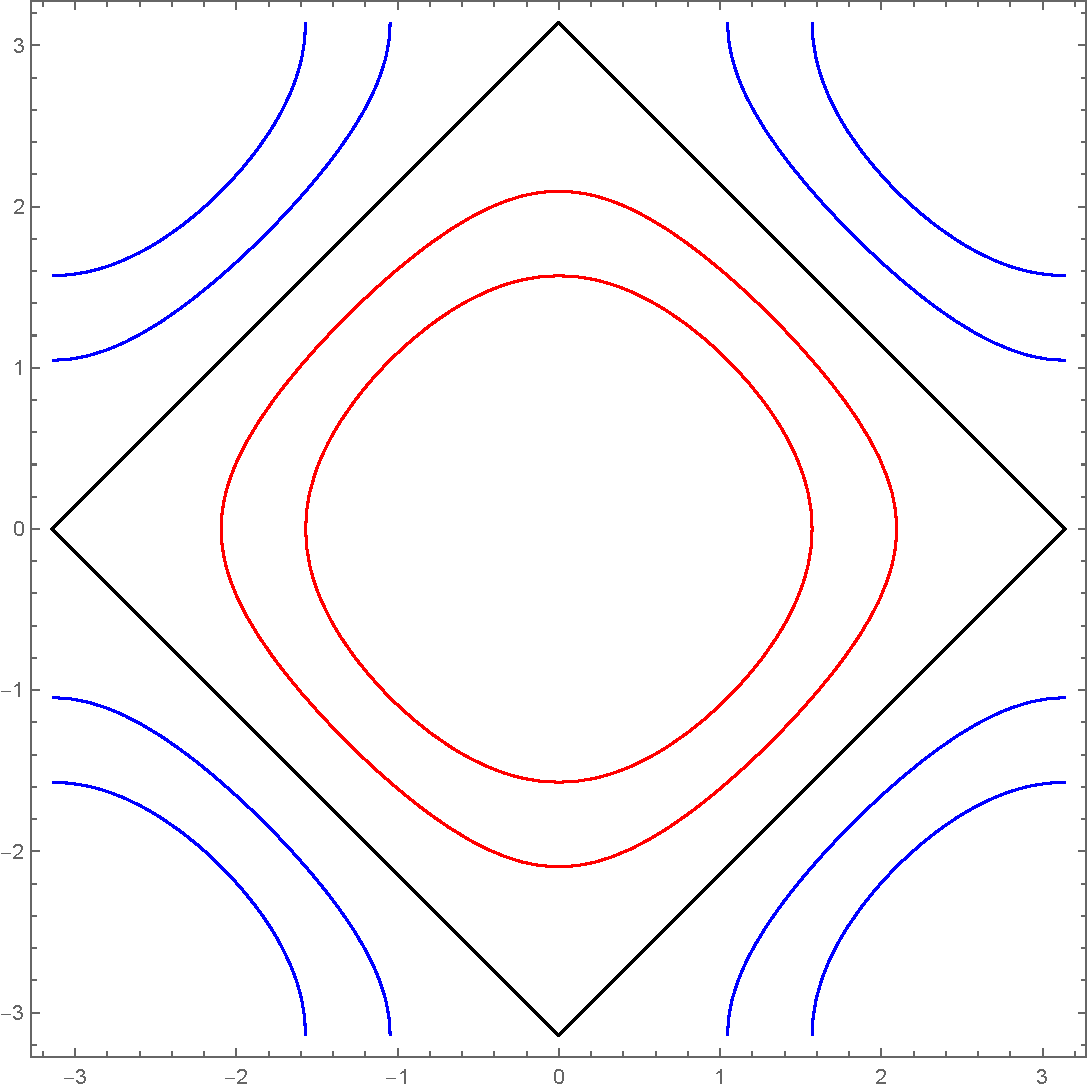
\includegraphics[width=0.6\textwidth]{figures/square_3d_bz_fermi_surface.pdf}
\end{center}

\subsection{Graphene}

The primitive unit vectors for Graphene are,
\[ \ve a_{1} = \f{a}{2} \br{\hat x + \sqrt{3} \hat y} \qquad \ve a_{2} = \f{a}{2} \br{-\hat x + \sqrt{3} \hat y} \eq \label{eq:gp_graphen_a} \]
Where the lattice structure is as follows,
\begin{center}
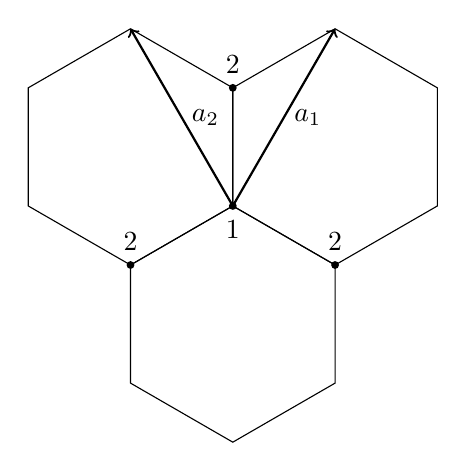
\begin{tikzpicture}
    \pgfmathsetmacro{\size}{1.5};
    \pgfmathsetmacro{\f}{sqrt(3)/2};
    \pgfmathsetmacro{\ss}{1/2};
    \draw (0,0) node[circle, inner sep=1pt, fill=black, label={below:$1$}]{};
    \draw (0,\size) node[circle, inner sep=1pt, fill=black, label={above:$2$}]{};
    \draw (\f*\size,-\ss*\size) node[circle, inner sep=1pt, fill=black, label={above:$2$}]{};
    \draw (-\f*\size,-\ss*\size) node[circle, inner sep=1pt, fill=black, label={above:$2$}]{};
    \draw (0,0) -- ++(\f*\size,-\ss*\size) -- ++(\f*\size,\ss*\size) -- ++(0, \size) -- ++(-\f*\size,\ss*\size) -- ++(-\f*\size,-\ss*\size) -- cycle;
    \draw (0,0) -- ++(0, \size) -- ++(-\f*\size,\ss*\size) -- ++(-\f*\size,-\ss*\size) --++(0, -\size) -- ++(\f*\size,-\ss*\size) -- ++(\f*\size,\ss*\size) -- cycle;
    \draw (0,0)  -- ++(-\f*\size,-\ss*\size) --++(0, -\size) -- ++(\f*\size,-\ss*\size) -- ++(\f*\size,\ss*\size) -- ++(0, \size) -- cycle;
    \draw[thick, ->] (0,0) -- node[right]{$\ve a_1$} ++(0+\f*\size, \size+\ss*\size);
    \draw[thick, ->] (0,0) -- node[right]{$\ve a_2$} ++(0-\f*\size, \size+\ss*\size);
\end{tikzpicture}
\end{center}

\[ \ve b_{1} = \f{2 \pi}{a\sqrt{3}} \br{\sqrt{3} \hat x +  \hat y} \qquad \ve b_{2} = \f{2 \pi}{a\sqrt{3}} \br{-\sqrt{3}\hat x +  \hat y} \eq \label{eq:gp_graphen_b}\]
The nearest neighbor Hamiltonian becomes,
\[ H = -t \sum_{\ve R} \br{\ket{\ve R, 2} \bra{\ve R, 1} + \ket{\ve R - \ve a_{1}, 2}\bra{\ve R, 1} + \ket{\ve R - \ve a_2, 2}\bra{\ve R, 1} + \text{h.c.}}\eq \label{eq:gp_graphene_H_nn} \]
In the reciprocal lattice,
\[ \ket{\ve R, \al} = \f{1}{\sqrt{N}} \sum_{\ve R} \ket{\ve k, \al} e^{-i \ve k \cdot \ve R} \]
Therefore the Hamiltonian becomes,
\begin{align*}
    H
    &= -\f{t}{N} \sum_{\ve R}\sum_{\ve k, \ve k'} \Bigg( \ket{\ve k, 2}\bra{\ve k,1}e^{-i \ve k \cdot \ve R} e^{i \ve k' \cdot \ve R} + \ket{\ve k, 2}\bra{\ve k,1}e^{-i \ve k \cdot \br{\ve R - \ve a_1}} e^{i \ve k' \cdot \ve R}+ \ket{\ve k, 2}\bra{\ve k,1}e^{-i \ve k \cdot \br{\ve R - \ve a_2}} e^{i \ve k' \cdot \ve R} + \text{h.c.} \Bigg) \\
\end{align*}
\[ H = - t\sum_{\ve k}\bs{\ket{\ve k, 2} \bra{\ve k, 1} \br{1 + e^{i \ve k \cdot \ve a_1} + e^{i \ve k \cdot \ve a_2}} + \ket{\ve k, 1} \bra{\ve k, 2} \br{1 + e^{-i \ve k \cdot \ve a_1} + e^{-i \ve k \cdot \ve a_2}}} \]
We have now diagonalized $H$ in terms of the momentum wave-vector index $\ve k$. Letting $H = \sum_{\ve k} H\br{\ve k}$ where,
\[ H\br{\ve k} = -t\bs{\ket{ 2} \bra{ 1} \br{1 + e^{i \ve k \cdot \ve a_1} + e^{i \ve k \cdot \ve a_2}} + \ket{ 1} \bra{ 2} \br{1 + e^{-i \ve k \cdot \ve a_1} + e^{-i \ve k \cdot \ve a_2}}} \]
Invoking pseudo-spin states $\ket{1} = \ket{\uu}$ and $\ket{2} = \ket{\dd}$ we can write,
\[ H\br{\ve k} = \ve d\br{\ve k} \cdot \ve \si \]
Where $\ve d \br{\ve k}$ is,
\begin{align*}
    d^{x}\br{\ve k} & = -t \bs{1 + \cos\br{\ve k \cdot \ve a_1} + \cos \br{\ve k \cdot \ve a_2}} \\
    d^{y}\br{\ve k} & = -t \bs{\sin\br{\ve k \cdot \ve a_1} + \sin \br{\ve k \cdot \ve a_2}} \\
    d^{z}\br{\ve k} & = 0
\end{align*}
The eigenvalues of $H\br{\ve k}$ are then the usual,
\[ \vep_{\pm}\br{\ve k} = \pm \abs{\ve d\br{\ve k}} \]
Since we have $1$ electron per carbon atom, there are 2 electrons per unit cell which means that the $\vep_{-}$ band is completely filled while the $\vep_{+}$ is empty. For this configuration, the conduction band is empty and thus graphene is an insulator. \\

In order to analyze the electronic structure of graphene, we need to rewrite $\ve k$ which is expressed via the reciprocal lattice vectors $\ve b_1, \ve b_2$ in terms of the Cartesian vectors $\ve a_1, \ve a_2$.
\[ \ve k = k_1 \ve b_1 + k_2 \ve b_2 \]
\[ \ve k \cdot \ve a_1 = \br{k_1 \ve b_1 + k_2 \ve b_2} \cdot \ve a_1 = 2 \pi k_1 \qquad \ve k \cdot \ve a_2 = 2 \pi k_2 \]
Recalling \cref{eq:gp_graphen_a,eq:gp_graphen_b},
\[ \ve a_{1} = \f{a}{2} \br{\hat x + \sqrt{3} \hat y} \qquad \ve a_{2} = \f{a}{2} \br{-\hat x + \sqrt{3} \hat y} \]
\[ \ve b_{1} = \f{2 \pi}{a\sqrt{3}} \br{\sqrt{3} \hat x +  \hat y} \qquad \ve b_{2} = \f{2 \pi}{a\sqrt{3}} \br{-\sqrt{3}\hat x +  \hat y}\]
We can now write $k_x, k_y$ in terms of $k_1, k_2$,
\[ k_x = \f{2 \pi }{\sqrt{3}a} \br{k_1 - k_2} \qquad k_y = \f{2 \pi}{\sqrt{3}a} \br{k_1 + k_2} \]
Inverting this system gives,
\[ k_1 = \f{a}{4 \pi} \br{k_x + \sqrt{3} k_y} \qquad k_2 = \f{a}{4 \pi} \br{-k_x + \sqrt{3} k_y} \]
Therefore,
\begin{align*}
    d^{x}\br{\ve k}
    &= - t\bs{1 + \cos\br{2 \pi k_1} + \cos\br{2 \pi k_2}} \\
    &= - t\bs{1 + 2\cos\br{\f{k_xa}{2}}\cos\br{\f{\sqrt{3}k_ya}{2}}}
\end{align*}
Similarly for $d^{y}\br{\ve k}$,
\[ d^{y}\br{\ve k} = -2 t \cos\br{\f{k_x a}{2}} \sin\br{\f{\sqrt{3} k_y a}{2}} \]
By examining these equations it can be seen that there are two points (and only two points) in the first Brillouin zone where both $d^{x}$ and $d^y$ vanish simultaneously. We label these points as $\ve k_{\pm}$,
\[ \ve k_+ = \br{k_{+, x}, k_{+, y}} = \br{\f{4 \pi }{3a}, 0} \]
\[ \ve k_- = \br{k_{-, x}, k_{-, y}} = \br{-\f{4 \pi }{3a}, 0} \]
At either of these points,
\[ \abs{\ve d \br{\ve k_{\pm}}} = \sqrt{{d^x}^2\br{\ve k} + {d^y}^2\br{\ve k}} = 0 \]
Therefore, the gap between the $\vep_{+}$ band and the $\vep_{-}$ closes at only two points. Since graphene is an insulator and does not have a Fermi surface (meaning its \textit{not} a metal) we refer to graphene, and materials that share these features, as \term{semimetals}. \\


The Brillouin zone of graphene can be derived using \cref{eq:gp_discrete_k} and \cref{eq:gp_kxky}. First, rewrite $\ve k$ which is typically defined in terms of the reciprocal lattice vectors $\ve b_1, \ve b_2$ in terms of the Cartesian vectors $\ve a_1, \ve a_2$.
\[ \ve k = k_1 \ve b_1 + k_2 \ve b_2 \qquad \ve b_i \cdot \ve a_j = 2 \pi \de_{ij}\]
\[ \ve k \cdot \ve a_1 = \br{k_1 \ve b_1 + k_2 \ve b_2} \cdot \ve a_1 = 2 \pi k_1 \qquad \ve k \cdot \ve a_2 = 2 \pi k_2 \]
Therefore using \cref{eq:gp_kxky} yields,

\begin{align*}
\eq \label{eq:gp_k1k2}
\begin{split}
k_1 &= \f{a}{4 \pi}\br{k_x + \sqrt{3}k_y} \\
k_2 &= \f{a}{4 \pi}\br{-k_x + \sqrt{3}k_y}
\end{split}
\end{align*}
Recalling \cref{eq:gp_graphene_a},
\[ \ve a_{1} = \f{a}{2} \br{\hat x + \sqrt{3} \hat y} \qquad \ve a_{2} = \f{a}{2} \br{-\hat x + \sqrt{3} \hat y} \]
\[ \ve b_{1} = \f{2 \pi}{a\sqrt{3}} \br{\sqrt{3} \hat x +  \hat y} \qquad \ve b_{2} = \f{2 \pi}{a\sqrt{3}} \br{-\sqrt{3}\hat x +  \hat y}\]
We can now write $k_x, k_y$ in terms of $k_1, k_2$,
\[ k_x = \f{2 \pi }{a} \br{k_1 - k_2} \qquad k_y = \f{2 \pi}{\sqrt{3}a} \br{k_1 + k_2} \]
Using \cref{eq:gp_periodic_boundary},
\[ 1 = e^{i N_i \ve k \cdot \ve a_i} \implies N_i \ve k \cdot \ve a_i = N_i 2 \pi k_i = 2 \pi m_i \implies N_i k_i = m_i \]
% \[ \abs{\ve b}^2 \leq 4\f{\br{2 \pi}^2}{a^2} \]
% \[ -2\f{\br{2 \pi}}{a} \leq \abs{\ve b} \leq 2\f{\br{2 \pi}}{a} \]
% Therefore,
% \[ 2N_i k_i = m_i \in \Z \]
Where $m_i \in \Z$ is an integer and $i \in \bc{1,2}$.\\

Moreover, since there are $N_i$ unit cells in the $\ve a_i$ direction we have,
\[ - \f{N_i}{2} \leq m_i < \f{N_i}{2} \qquad m_i \in \Z, \forall i \in \bc{1,2} \]
Therefore,
\[ - \f{N_i}{2} \leq N_i k_i < \f{N_i}{2} \qquad \forall i \in \bc{1,2} \]
\[ - \f{1}{2} \leq k_i < \f{1}{2} \qquad \forall i \in \bc{1,2} \]
This result is intuitive. The first Brillouin zone only extends halfway in the direction of $\ve b_1, \ve b_2$ or combinations thereof. These inequalities yield the following,
\[ \abs{k_1}, \abs{k_2} < \f12  \]
\[ \ve k = k_x \hat x + k_y \hat y  \]
Where the norms of $\ve b_i$ are independent of $i$.
\[ b^2 = \abs{\ve b_1}^2 = \abs{\ve b_2}^2 =  4\f{\br{2 \pi}^2}{3a^2} = \f{16 \pi^2}{3a^2}\]
\[ \f12 \leq \f{\ve k \cdot \ve b_i}{b^2} = k_i \leq \f12  \]
Therefore,
\[ -\f12 \leq \f{1}{b^2} \br{\f{2 \pi}{a\sqrt{3}} \br{\sqrt{3} \hat x +  \hat y}} \cdot \br{k_x \hat x + k_y \hat y} \leq \f12  \]
\[ -\f12 \leq \f{3a^2}{4\br{2 \pi}^2} \br{\f{2 \pi}{a\sqrt{3}} \br{\sqrt{3} k_x +  k_y}} \leq \f12  \]
\[ -\f{4}{\sqrt{3}}\pi \leq  a\br{\sqrt{3} k_x +  k_y} \leq \f{4}{\sqrt{3}}\pi  \]
Similarly,
\[ -\f{4}{\sqrt{3}}\pi \leq  a\br{-\sqrt{3} k_x +  k_y} \leq \f{4}{\sqrt{3}}\pi  \]
And the positive sum of these two inequalities gives,
\[ -\f{4}{\sqrt{3}}\pi \leq  ak_y \leq \f{4}{\sqrt{3}}\pi  \]
Which does not constrain the first Brillouin zone any further. Instead we invoke,
\[ \f12 \leq \f{\ve k \cdot \br{\ve b_1 + \ve b_2}}{b^2} \leq \f12  \]
Which becomes,
\[ -\f{4}{\sqrt{3}}\pi \leq 2ak_y \leq \f{4}{\sqrt{3}}\pi  \]
Therefore the Brillouin zone is fully characterized.
\begin{center}
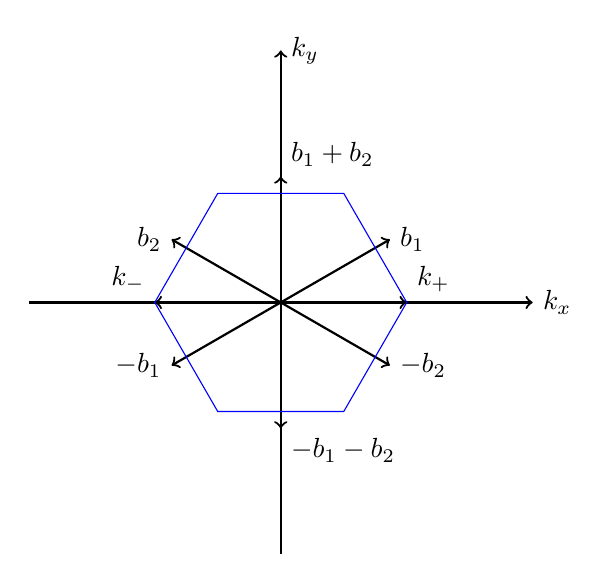
\begin{tikzpicture}[scale=0.8]
    \pgfmathsetmacro{\plot}{4};
    \pgfmathsetmacro{\st}{sqrt(3)};
    \pgfmathsetmacro{\size}{3};
    \draw[thick,->] (-\plot, 0) -- (\plot, 0) node[right]{$k_x$};
    \draw[thick,->] (0, -\plot) -- (0, \plot) node[right]{$k_y$};
    \draw[thick,->] (0,0) -- (\st, 1)         node[right]{$\ve b_1$};
    \draw[thick,->] (0,0) -- (-\st, 1)        node[left]{$\ve b_2$};
    \draw[thick,->] (0,0) -- (\st, -1)        node[right]{$-\ve b_2$};
    \draw[thick,->] (0,0) -- (-\st, -1)       node[left]{$-\ve b_1$};
    \draw[thick,->] (0,0) -- (0, -2)          node[below right]{$-\ve b_1 -\ve b_2$};
    \draw[thick,->] (0,0) -- (0, 2)           node[above right]{$\ve b_1 +\ve b_2$};
    \draw[thick,->] (0,0) -- (2/3*\size, 0)   node[above right]{$\ve k_+$};
    \draw[thick,->] (0,0) -- (-2/3*\size, 0)  node[above left]{$\ve k_-$};
    \draw[blue]
    (2/3*\size, 0) --
    (1, \st)       --
    % (0, 2*\st)     --
    (-1, \st)      --
    (-2/3*\size, 0)--
    % (0, -2*\st)    --
    (-1, -\st)     --
    (1, -\st)      --
    cycle;
\end{tikzpicture}
\end{center}
\begin{center}
    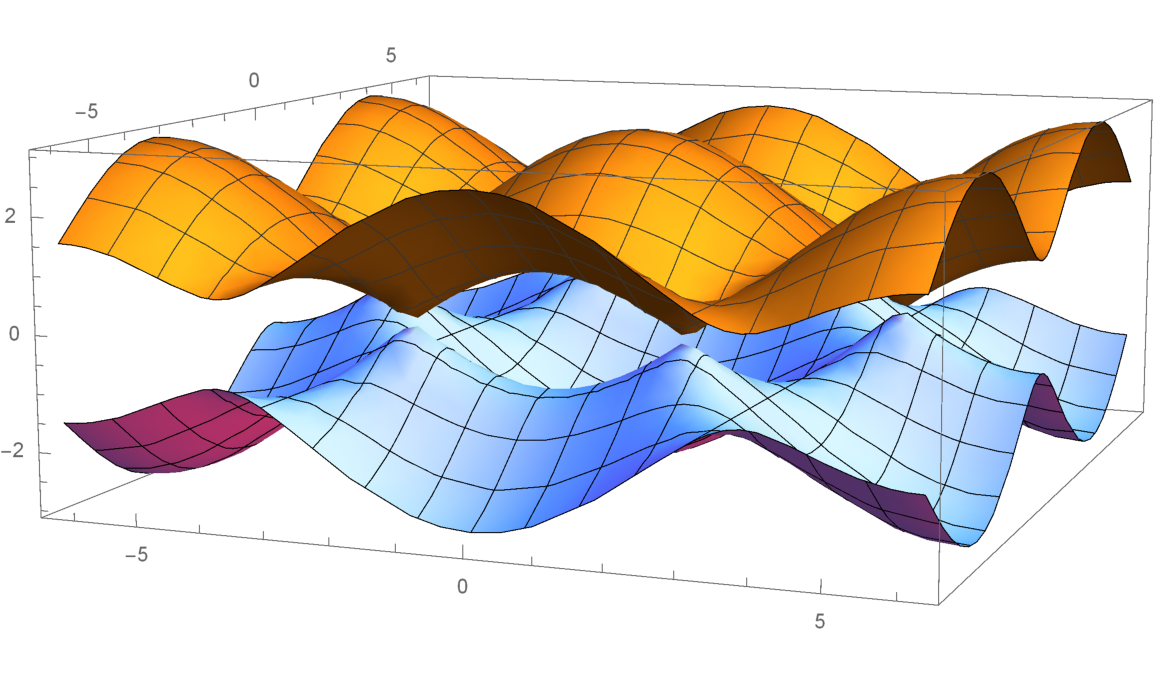
\includegraphics[width=0.45\linewidth]{figures/graphene_3d_dr.pdf}
    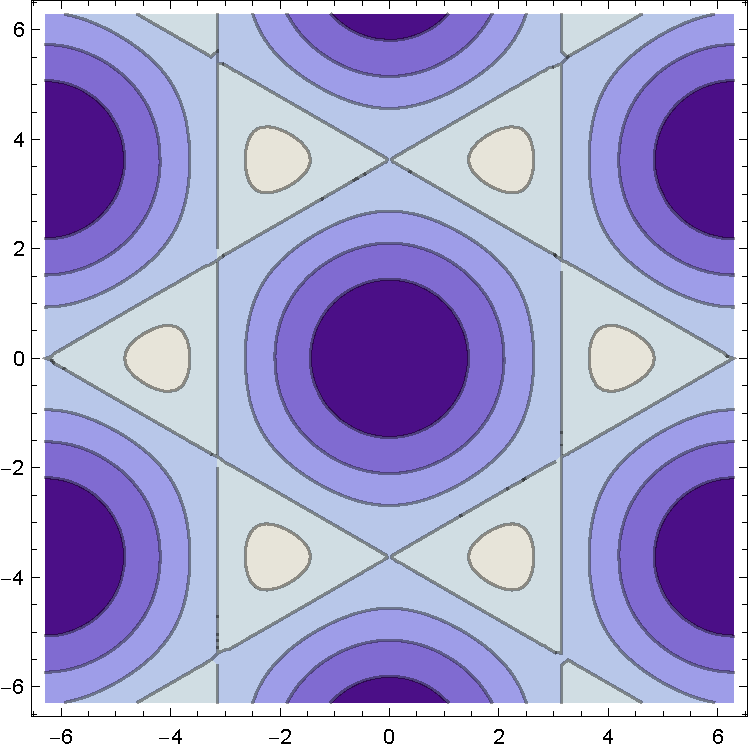
\includegraphics[width=0.25\linewidth]{figures/graphene_3d_contour_dr.pdf}
    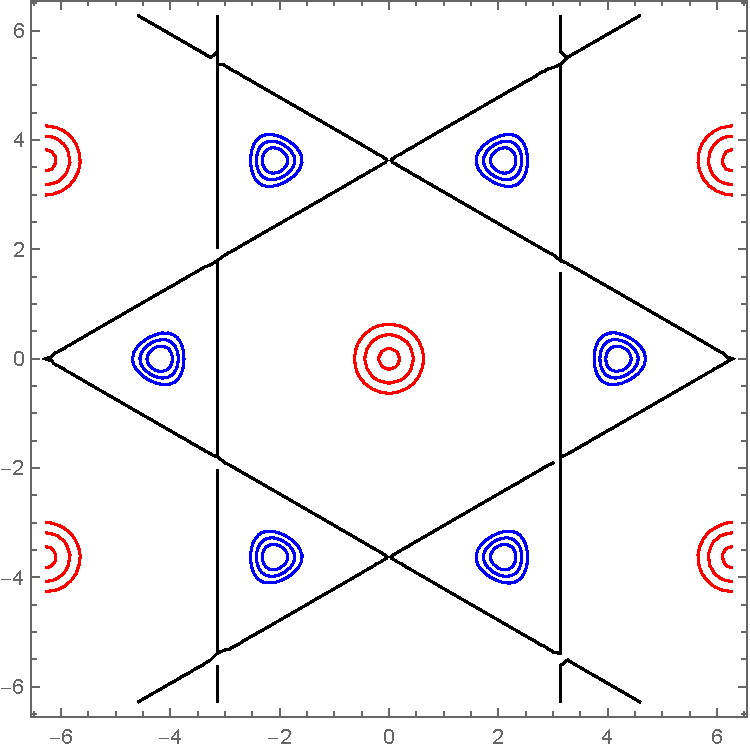
\includegraphics[width=0.25\linewidth]{figures/graphene_3d_contour_bz.pdf}
\end{center}
The first Brillouin zone for graphene forms a hexagonal lattice with the corners obtained from $\ve k_{\pm}$ by adding $\pm b_1, \pm b_2$,
\[ \ve G = m_1 \ve b_2 + m_2 \ve b_2 \]
In graphene, the upper and lower band are \textit{not} separated by a band gap (sometimes $\vep_{+} > \vep_{-}$ and sometimes $\vep_{+} < \vep_{-}$). The crossing points are precisely the two points where $\ve k = \ve k_{\pm}$. If we expand $H\br{\ve k}$ near $\ve k_{\pm}$ to first order,
\[ k_x = k_{x, \pm} + \de k_x  \qquad k_y = \de k_y\]
To first order,
\[ d^{x}_{\pm} \br{\de \ve k} \simeq \pm \f{\sqrt{3}}{2} t a \de k_x \]
\[ d^{y}_{\pm} \br{\de \ve k} \simeq \f{\sqrt{3}}{2} t a \de k_y \]
For both the $x$ and $y$ directions, the leading coefficient $\f{\sqrt{3}}{2} t a$ has units of speed times $\hbar$. We again call this the Fermi velocity,
\[ v\tsb{F} = \f{\sqrt{3} t a}{2\hbar} \]
Then we can write the Hamiltonian as,
\[ H_{\pm}\br{\ve k} = \hbar v\tsb{F} \br{\pm k_x \si^x + k_y \si^{y}} \eq \label{eq:gp_2d_dirac}\]
Where here $k_x$ and $k_y$ refer to $\de k_x$ and $\de k_y$. This is done by shifting coordinates such that $\ve k_{\pm} = 0$ for each of the $+, -$ cases. Upon examination of \cref{eq:gp_2d_dirac}, \cref{eq:gp_2d_dirac} takes the form of a 2D Dirac Hamiltonian for a massless relativistic particle in 2D. The energies near the touching points $\ve k_{\pm}$ is,
\[ \vep\br{\ve k} = \pm \hbar v\tsb{F} k \]
Where $k = \sqrt{k_x^2 + k_y^2}$. This means that $\vep\br{\ve k}$ has linear dispersion near $\ve k_{\pm}$. \\

One question we can ask is what can we do to graphene in order to open a gap between $\ve k_{-}$ and $\ve k_{+}$. In order words, how can we give the electron in \cref{eq:gp_2d_dirac} an effective mass. This can be accomplished by introducing a discrepancy between the atoms labeled $1$ and the atoms labeled $2$ within a unit cell. As an example, we can add energies $\pm m$ to the atoms as follows,

\begin{center}
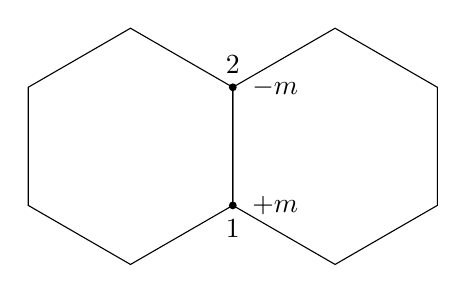
\begin{tikzpicture}
    \pgfmathsetmacro{\size}{1.5};
    \pgfmathsetmacro{\f}{sqrt(3)/2};
    \pgfmathsetmacro{\ss}{1/2};
    \draw (0,0) node[circle, inner sep=1pt, fill=black, label={below:$1$}]{};
    \draw (0,\size) node[circle, inner sep=1pt, fill=black, label={above:$2$}]{};
    \draw (0,\size) node[label={right:$-m$}]{};
    \draw (0,0) node[label={right:$+m$}]{};
    % \draw (\f*\size,-\ss*\size) node[circle, inner sep=1pt, fill=black, label={above:$2$}]{};
    % \draw (-\f*\size,-\ss*\size) node[circle, inner sep=1pt, fill=black, label={above:$2$}]{};
    \draw (0,0) -- ++(\f*\size,-\ss*\size) -- ++(\f*\size,\ss*\size) -- ++(0, \size) -- ++(-\f*\size,\ss*\size) -- ++(-\f*\size,-\ss*\size) -- cycle;
    \draw (0,0) -- ++(0, \size) -- ++(-\f*\size,\ss*\size) -- ++(-\f*\size,-\ss*\size) --++(0, -\size) -- ++(\f*\size,-\ss*\size) -- ++(\f*\size,\ss*\size) -- cycle;
    % \draw (0,0)  -- ++(-\f*\size,-\ss*\size) --++(0, -\size) -- ++(\f*\size,-\ss*\size) -- ++(\f*\size,\ss*\size) -- ++(0, \size) -- cycle;
    % \draw[thick, ->] (0,0) -- node[right]{$\ve a_1$} ++(0+\f*\size, \size+\ss*\size);
    % \draw[thick, ->] (0,0) -- node[right]{$\ve a_2$} ++(0-\f*\size, \size+\ss*\size);
\end{tikzpicture}
\end{center}

Which effectively corresponds to adding the following term to the original Hamiltonian,
\[ H' = m \sum_{\ve R} \br{\ket{\ve R, 1}\bra{\ve R, 1} - \ket{\ve R, 2}\bra{\ve R, 2}} \]


Applying the Fourier transform yields the following,
\[ H' = m \sum_{\ve k} \br{\ket{\ve k, 1}\bra{\ve k, 1} - \ket{\ve k, 2}\bra{\ve k, 2}} \]
Which further adjusts the dispersion relationship,
\[ H'\br{\ve k} = m \br{\ket{1}\bra{1} - \ket{2}\bra{2}} = m \si^{z} \]
Therefore,
\[ H_{\pm}\br{\ve k} =\hbar v\tsb{F} \br{\pm k_x \si^x + k_y \si^{y}} + m\si^{z} \]
\[ \vep_{\pm} \br{\ve k} = \pm \sqrt{\hbar^2 v\tsb{F}^2 k^2 + m^2} \]
This opens up a band gap of size $2m$. Therefore clean graphene ($m=0$) is a semimetal due to inversion symmetry but becomes an insulator for $m > 0$. \\

Returning to the case of $m=0$,
\[ H_{\pm}\br{\ve k} =\hbar v\tsb{F} \br{\pm k_x \si^x + k_y \si^{y}} \]
The `$\pm$' can be thought of as a two component degree of freedom. Because there are two components, we can think of `$\pm$' as another pseudo-spin value $\tau$.
\begin{align*}
    \tau^{z} &= \ket{+} \bra{+} - \ket{-}\bra{-} \\
    \tau^{y} &= -i\br{\ket{+} \bra{-} - \ket{-}\bra{+}} \\
    \tau^{x} &= \ket{+} \bra{-} + \ket{-}\bra{+}
\end{align*}
Which means that the Hamiltonian can be written without the `$\pm$' as a single matrix,
\[ H\br{\ve k} =\hbar v\tsb{F} \br{k_x \tau^{z} \si^x + k_y \si^{y}} \eq \label{eq:gp_double2spin}\]

\subsubsection{Spin-Orbit Interactions}
\label{sec:soi}
What are the symmetries of \cref{eq:gp_double2spin}? We must have the following:
\begin{enumerate}
    \item Time Reversal Symmetry
    \item Inversion Symmetry
\end{enumerate}
In order to facilitate discussions, we introduce two operators; the \term{inversion (parity) operator $\pi$} and \term{time-reversal operator $\Theta$}. The symmetries of \cref{eq:gp_double2spin} can we written,
\[  \pi^{\dagger} H\br{\ve k} \pi = H\br{\ve k} \eq \label{eq:gp_parity_graphene}\]
\[  \Theta H\br{\ve k} \Theta^{-1} = H\br{\ve k} \eq \label{eq:gp_tr_graphene}\]
Since $\tau^{z}$ refers to the two band touching points (coordinates in momentum space), $\tau^{z}$ changes sign under both symmetries,
\[ \pi^{\dagger} \tau^{z} \pi = - \tau^{z} \eq \label{eq:gp_tau_z_sym_parity}\]
\[ \Theta \tau^{z} \Theta^{-1} = - \tau^{z} \eq \label{eq:gp_tau_z_sym_tr}\]
Furthermore, $k_{x, y, z}$ represent momentum and is thus time and parity odd,
\[ \pi^{\dagger} k_{x,y,z} \pi = - k_{x,y,z} \]
\[ \Theta k_{x,y,z} \Theta^{-1} = - k_{x,y,z} \]
Therefore we must conclude that $\si^{x}$ is even under these symmetries and $\si^{y}$ is odd pursuant to \cref{eq:gp_parity_graphene,eq:gp_tr_graphene},
\[ \pi^{\dagger} \si^{y} \pi = - \si^{y} \]
\[ \Theta \si^{y} \Theta^{-1} = - \si^{y} \]
\[ \pi^{\dagger} \si^{x} \pi = + \si^{x} \]
\[ \Theta \si^{x} \Theta^{-1} = + \si^{x} \]
This is intuitive because $\si$ refers to the spatial location of atoms $1$ and $2$ oriented in the $y$ direction.
If we were to include the massive term $m\si^{z}$ we break symmetry in \cref{eq:gp_parity_graphene,eq:gp_tr_graphene},
\[ \pi^{\dagger} \si^{z} \pi = - \si^{z} \qquad \Theta \si^{z} \Theta^{-1} = \si^{z} \eq \label{eq:gp_si_z_sym}\]
Specifically, $m \si^{z}$ breaks inversion symmetry. This is intuitive because $m$ adds spatial discrepancies between $1$ and $2$. Can we open a gap in graphene without breaking time-reversal or inversion symmetries?\\

Interestingly, this lack of symmetry is an artifact of the simplistic model introduced by \cref{eq:gp_graphene_H_nn}. If we include \textit{next-nearest neighbor} terms, it is possible to recover symmetries. Upon examination of \cref{eq:gp_si_z_sym} and \cref{eq:gp_tau_z_sym_parity,eq:gp_tau_z_sym_tr} we find that $\tau^{z} \si^{z}$ is invariant under inversion,
\[ \pi^{\dagger} \tau^{z} \si^{z} \pi = \tau^{z} \si^{z} \]
But $\tau^{z} \si^{z}$ is not invariant under time-reversal,
\[ \Theta \tau^{z} \si^{z} \Theta^{-1} = -\tau^{z} \si^{z} \]
Other component that is missing from our model is the real spin of the electron (not pseudo-spin) $\ve S$. Spin $\ve S$ is parity even and time-reversal odd,
\[ \pi^{\dagger} \ve S \pi = \ve S \qquad \Theta \ve S \Theta^{-1} = - \ve S \]
\begin{align*}
    S^{z} &= \ket{\uu} \bra{\uu} - \ket{\dd}\bra{\dd} \\
    S^{y} &= -i\br{\ket{\uu} \bra{\dd} - \ket{\dd}\bra{\uu}} \\
    S^{x} &= \ket{\uu} \bra{\dd} + \ket{\dd}\bra{\uu}
\end{align*}
Upon adding this term, $\tau^{z} \si^{z} S^{z}$ maintains the desired symmetries,
\[ \pi^{\dagger} \tau^{z} \si^{z} S^{z} \pi = \tau^{z} \si^{z} S^{z} \qquad \Theta \tau^{z} \si^{z} S^{z} \Theta^{-1} = \tau^{z} \si^{z} S^{z} \]
This was discovered by Kane and Mele (2005) and their paper gave rise to the field of topological insulators. Therefore the true graphene Hamiltonian can be written as,
\[ H\br{\ve k} =\hbar v\tsb{F} \br{k_x \tau^{z} \si^x + k_y \si^{y}} + \De\tsb{SO} \tau^{z} \si^{z} S^{z} \eq \label{eq:gp_kane_mele}\]
Where $\De\tsb{SO}$ is referred to as the \term{spin-orbit interaction}. The origin of the $\De\tsb{SO}$ term is due to the following process. When the valence electrons have the ability to tunnel between atoms, some of the atoms in the crystal lattice become ionized. The electric field of ionized atoms is felt as a magnetic field in the rest frame of the electrons. Effectively this magnetic field has strength $\ve B = \ve v \times \ve E / c$ which tends to be small as $B \propto c^{-1}$. Additionally, $\ve E$ grows for heavier and heavier atoms. This magnetic field acts on the spin in the usual manner $H \propto \ve B \cdot \ve S$. This is encapsulated in \cref{eq:gp_kane_mele} as $\tau^{z} \si^{z}$ is coupled with the spin $S^{z}$. \\

In order to formally introduce the $\De\tsb{SO} \tau^{z} \si^{z} S^{z}$ term into the Hamiltonian, we need to include next nearest-neighbor tunneling ($1 \to 1$ and $2 \to 2$ tunneling),

\begin{center}
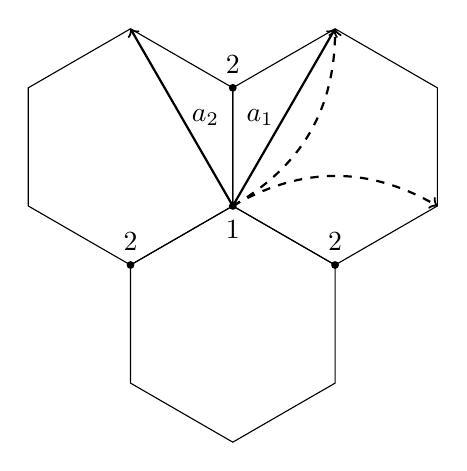
\begin{tikzpicture}
    \pgfmathsetmacro{\size}{1.5};
    \pgfmathsetmacro{\f}{sqrt(3)/2};
    \pgfmathsetmacro{\ss}{1/2};
    \draw (0,0) node[circle, inner sep=1pt, fill=black, label={below:$1$}]{};
    \draw (0,\size) node[circle, inner sep=1pt, fill=black, label={above:$2$}]{};
    \draw (\f*\size,-\ss*\size) node[circle, inner sep=1pt, fill=black, label={above:$2$}]{};
    \draw (-\f*\size,-\ss*\size) node[circle, inner sep=1pt, fill=black, label={above:$2$}]{};
    \draw (0,0) -- ++(\f*\size,-\ss*\size) -- ++(\f*\size,\ss*\size) -- ++(0, \size) -- ++(-\f*\size,\ss*\size) -- ++(-\f*\size,-\ss*\size) -- cycle;
    \draw (0,0) -- ++(0, \size) -- ++(-\f*\size,\ss*\size) -- ++(-\f*\size,-\ss*\size) --++(0, -\size) -- ++(\f*\size,-\ss*\size) -- ++(\f*\size,\ss*\size) -- cycle;
    \draw (0,0)  -- ++(-\f*\size,-\ss*\size) --++(0, -\size) -- ++(\f*\size,-\ss*\size) -- ++(\f*\size,\ss*\size) -- ++(0, \size) -- cycle;
    \draw[thick, ->] (0,0) -- node[left]{$\ve a_1$} ++(0+\f*\size, \size+\ss*\size);
    \draw[thick, ->] (0,0) -- node[right]{$\ve a_2$} ++(0-\f*\size, \size+\ss*\size);
    \path (0,0) edge[thick, draw, bend right, dashed, ->] ++(0+\f*\size, \size+\ss*\size);
    \path (0,0) edge[thick, draw, bend left, dashed, ->] ++(2*\f*\size, 0);
\end{tikzpicture}
\end{center}

The additional terms to \cref{eq:gp_graphene_H_nn} can be expressed as,
\[ H = \cdots -i t' \br{\ket{\ve R + \ve a_1 - \ve a_2, 1}\bra{\ve R, 1} - \ket{\ve R, 1} \bra{\ve R + \ve a_1 - \ve a_2, 1}} \cdots \]
Which has tunneling amplitude $i t'$. The intermediate negative sign is due to the tunneling amplitude being imaginary which switches signs under conjugation.\\


\subsubsection{Second Nearest-Neighbors}

\tikzstyle{atomoptions}=[draw, circle, inner sep=1pt, fill=#1]

\newcommand{\atomat}[2]{node[atomoptions={#1}] () at #2 {}}
\newcommand{\atom}[1]{\begin{tikzpicture}[baseline=-2pt]\draw\atomat{#1}{(0,0)};\end{tikzpicture}}
\newcommand{\hexgonat}[1]{
#1
-- ++(+\diagh,-\diagv)
-- ++(0, -\vert)
-- ++(-\diagh,-\diagv)
-- ++(-\diagh,+\diagv)
-- ++(0, +\vert)
-- ++(+\diagh,+\diagv)
}
\newcommand{\hexgonatatoms}[1]{
#1                  node[atomoptions={black}]{}
++(+\diagh,-\diagv) node[atomoptions={white}]{}
++(0, -\vert)       node[atomoptions={black}]{}
++(-\diagh,-\diagv) node[atomoptions={white}]{}
++(-\diagh,+\diagv) node[atomoptions={black}]{}
++(0, +\vert)       node[atomoptions={white}]{}
++(+\diagh,+\diagv) node[atomoptions={black}]{}
}
\newcommand{\atomm}{\atom{white}}
\newcommand{\atomp}{\atom{black}}

\begin{center}
\begin{tikzpicture}
    \pgfmathsetmacro{\edgelength}{1.5};
    \pgfmathsetmacro{\diagh}{sqrt(3)/2*\edgelength};
    \pgfmathsetmacro{\diagv}{1/2*\edgelength};
    \pgfmathsetmacro{\vert}{\edgelength};
    \pgfmathsetmacro{\feather}{0.2};
    \coordinate (a1) at (-\diagh, +\diagv+\vert);
    \coordinate (a2) at (+\diagh, +\diagv+\vert);
    \foreach \n/\m in {2/-1, -1/2, 2/0, 0/2, 0/-1,+1/-1,-1/0,0/0,+1/0,-1/+1,0/+1,+1/+1}{
        \draw[gray] \hexgonat{($\n*(a1) + \m*(a2)$)};
        \draw \hexgonatatoms{($\n*(a1) + \m*(a2)$)};
    }
    \foreach \n/\m in {2/-1, -1/2, 0/-1,+1/-1,-1/0,0/0,+1/0,-1/+1,0/+1, -1/-1, -2/+1, -2/+2, -2/0, +1/-2, +2/-2, 0/-2}{
        \draw[thick, red] plot [smooth cycle, tension=1, shift={($\n*(a1) + \m*(a2)$)}] coordinates {(-\feather,0) (+\feather,0) (+\feather,\vert) (-\feather,\vert)};
    }
    \draw[blue, fill=blue, fill opacity=0.05] \hexgonat{(0,+\vert)};
    \draw[<-] (+\diagh,0) to[in=0, out=0] (1,5) node[left]{Wigner-Seitz Unit Cell};
    \draw[thick, ->] (0,0) -- node[left ]{$\ve a_1$} ++(a1);
    \draw[thick, ->] (0,0) -- node[right]{$\ve a_2$} ++(a2);
    \draw[thick, dashed, green] (0, \vert) to[bend right] (-\diagh, -\diagv);
    \draw[thick, dashed, green] (0, \vert) to[bend right] (+\diagh, -\diagv);
    \draw[thick, dashed, green] (+\diagh, -\diagv) to[bend right] (0, \vert);
    \draw[thick, dashed, green] (+\diagh, -\diagv) to[bend left ] (-\diagh, -\diagv);
    \draw[thick, dashed, green] (-\diagh, -\diagv) to[bend right] (0, \vert);
    \draw[thick, dashed, green] (-\diagh, -\diagv) to[bend left ] (+\diagh, -\diagv);
    \draw[thick, dashed, green] (0,0) to[bend right] (a1);
    \draw[thick, dashed, green] (0,0) to[bend left ] (a2);
    \draw[thick, dashed, green] (0,0) to[bend left ] (a1);
    \draw[thick, dashed, green] (0,0) to[bend right] (a2);
    \draw[thick, dashed, green] (0,0) to[bend left ] ($-1*(a1) + 1*(a2)$);
    \draw[thick, dashed, green] (0,0) to[bend right] ($-1*(a1) + 1*(a2)$);
    \draw[thick, dashed, blue]  (0,0) to[bend left ] (0, \vert);
    \draw[thick, dashed, blue]  (0,0) to[bend left ] (+\diagh, -\diagv);
    \draw[thick, dashed, blue]  (0,0) to[bend left ] (-\diagh, -\diagv);
    \draw[thick, dashed, blue]  (0,0) to[bend right] (0, \vert);
    \draw[thick, dashed, blue]  (0,0) to[bend right] (+\diagh, -\diagv);
    \draw[thick, dashed, blue]  (0,0) to[bend right] (-\diagh, -\diagv);
\end{tikzpicture}
\end{center}
In the graphene lattice depicted above, each unit cell located at $\ve R = n_1 \ve a_1 + n_2 \ve a_2$ where $n_1, n_2 \in \Z$ has two atoms $\al \in \bc{\atomm, \atomp}$.
\[ \ve a_1 = \f{a}{2}\br{\hat x + \sqrt{3}\hat y} \qquad \ve a_2 = \f{a}{2}\br{-\hat x + \sqrt{3}\hat y} \]
An electron localized in the atom $\al \in \bc{\atomm, \atomp}$ at $\ve R$ is denoted as $\ket{\ve R, \al}$. \\

There are $6$ possible nearest-neighbor transitions illustrated in blue above. These transitions, with intensity $t_1$ can be written as the nearest-neighbor Hamiltonian $H_1$,
\[ H_1 = - t_1 \sum_{\ve R} \bc{\ket{\ve R, \atomm}\bra{\ve R, \atomp} + \ket{\ve R-\ve a_1, \atomm}\bra{\ve R, \atomp} + \ket{\ve R - \ve a_2, \atomm}\bra{\ve R, \atomp} + \text{h.c.}} \]
There are $12$ possible next-nearest-neighbor transitions illustrated in green above. These transitions, with intensity $t_2$ can be written as the nearest-neighbor Hamiltonian $H_2$ (note that these transitions were all defined in the same direction; this is important when we invoke $t_2 = i \ti t_2, \ti t_2 \in \R$ later),
\begin{align*}
H_{2, \atomm} &= - t_2 \sum_{\ve R} \bc{\ket{\ve R+\ve a_1, \atomm}\bra{\ve R, \atomm} + \ket{\ve R-\ve a_2, \atomm}\bra{\ve R, \atomm}+ \ket{\ve R-\ve a_1, \atomm}\bra{\ve R-\ve a_2, \atomm} + \text{h.c.}} \\
H_{2, \atomp} &= -t_2 \sum_{\ve R} \bc{\ket{\ve R+\ve a_1, \atomp}\bra{\ve R, \atomp} + \ket{\ve R, \atomp}\bra{\ve R+\ve a_2, \atomp}+ \ket{\ve R-\ve a_1, \atomp}\bra{\ve R-\ve a_2, \atomp} + \text{h.c.}}
\end{align*}
Altogether,
\[ H = H_1 + H_2 = H_1 + H_{2, \atomp} + H_{2, \atomm} \eq \label{eq:gp_hamiltonian_total}\]

In order to diagonalize \cref{eq:gp_hamiltonian_total} with respect to $\ve R$, we may switch to momentum space,
\[ \ket{\ve R, \al} =  \sum_{\ve R} \ket{\ve k, \al}\braket{\ve k, \al}{\ve R, \al} \qquad \forall \al \in \bc{\atomp, \atomm} \eq \label{eq:gp_basis_change}\]
Where $\braket{\ve k, \al}{\ve R, \al}$ is defined and normalized independent of $\al$. Motivated by free electrons, $\braket{k}{x} \propto e^{-ikx}$ we map $x$ to the position in the crystal:
\begin{align*}
    \eq \label{eq:gp_xk}
    \begin{split}
        x \mapsto n_1 \ve a_1 + n_2 \ve a_2 &= \ve R\\
        k \mapsto k_1 \f{\ve a_1}{a} + k_2 \f{\ve a_2}{a} &= \ve k
    \end{split}
\end{align*}
Therefore,
\[ \braket{\ve k, \al}{\ve R, \al} \propto e^{i\ve k \cdot \ve R} \eq \label{eq:gp_plane_wave}\]
The normalization factor comes from completeness,
\[ \sum_{\ve R} \abs{\braket{\ve k, \al}{\ve R, \al}}^2 = 1 \eq \label{eq:gp_normalization}\]
Heretofore, no restrictions have been made on the range of $\ve R$. Evidently, a real substance will possess finite, albeit many, unit cells. To emulate this feature, equip this model with periodic boundary conditions such that there are $N_i$ distinct unit cells in the $\ve a_i$ direction. Therefore for all $\al, \ve R$,
\[ \ket{\ve R, \al} = \ket{\ve R + N_1 \ve a_1, \al} = \ket{\ve R + N_2 \ve a_2, \al} \eq \label{eq:gp_periodic_boundary}\]
Letting $\ga \in \R$ be the normalization coefficient in \cref{eq:gp_plane_wave}, \cref{eq:gp_normalization} becomes,
\[ 1 = \sum_{\ve R} \abs{\braket{\ve k, \al}{\ve R, \al}}^2 = \sum_{n_1 = 1}^{N_1}\sum_{n_2 = 1}^{N_2} \abs{\ga e^{i\ve k \cdot \ve R}}^2 = N_1 N_2 \ga^2 \implies \ga = \f{1}{\sqrt{N_1 N_2}}\]
Consequently, \cref{eq:gp_basis_change} can be written as follows,
\[ \ket{\ve R, \al} = \f{1}{\sqrt{N_1N_2}} \sum_{\ve k} e^{i \ve k \cdot \ve R} \ket{\ve k, \al} \eq \label{eq:gp_basis_coeffs}  \]
Additionally, the periodic boundary condition of \cref{eq:gp_periodic_boundary} gives,
\[ \ket{\ve R, \al} = \ket{\ve R + N_i \ve a_i, \al} = \f{1}{\sqrt{N_1N_2}} \sum_{\ve k} e^{i \ve k \cdot \br{\ve R + N_i \ve a_i}} \ket{\ve k, \al} = \f{1}{\sqrt{N_1N_2}} \sum_{\ve k} e^{i \ve k \cdot \ve R} \ket{\ve k, \al}  \]
Therefore $e^{i N_i \ve k \cdot \ve a_i} = e^{i 2N_i k_i a} = 1$ which gives,
\[ 2N_i k_i a = 2 \pi m_i \qquad m_i \in \Z, \forall i \in \bc{1,2} \]
\[ k_i = \f{\pi m_i}{N_i a} \qquad m_i \in \Z, \forall i \in \bc{1,2} \eq \label{eq:gp_discrete_k} \]
Therefore each of the $k_i$'s are discrete. Summing \cref{eq:gp_hamiltonian_total} over the momentum space $\ve k, \ve k'$ and using the following identity,
\[ \f{1}{N_1 N_2} \sum_{\ve R} e^{-i\br{\ve k-\ve k'} \cdot \ve R} = \de_{\ve k, \ve k'} \]
Yields,
\begin{align*}
H_1 &= - t_1 \sum_{\ve k} \bc{\ket{\ve k, \atomm}\bra{\ve k, \atomp}\bc{1 + e^{-i \ve k \cdot \ve a_1} + e^{-i \ve k \cdot \ve a_2}} + \text{h.c.}} \\
H_{2, \atomm} &= - t_2 \sum_{\ve k} \bc{\ket{\ve k, \atomm}\bra{\ve k, \atomm}\bc{e^{i \ve k \cdot \ve a_1} + e^{-i \ve k \cdot \ve a_2} + e^{i \ve k \cdot \br{\ve a_2 - \ve a_1}}} + \text{h.c.}} \\
H_{2, \atomp} &= -t_2 \sum_{\ve k} \bc{\ket{\ve k, \atomp}\bra{\ve k, \atomp}\bc{e^{i \ve k \cdot \ve a_1} + e^{-i \ve k \cdot \ve a_2} + e^{i \ve k \cdot \br{\ve a_2 - \ve a_1}}} + \text{h.c.}}
\end{align*}
Therefore $H = \sum_{\ve k}H\br{\ve k}$ gives,
\[ H\br{\ve k} = \sum_{\ve k} \br{-t_1  \bs{\ket{\atomm}\bra{\atomp}\bc{1 + e^{-i \ve k \cdot \ve a_1} + e^{-i \ve k \cdot \ve a_2}}} - t_2\bs{\br{\ket{\atomp}\bra{\atomp} + \ket{\atomm}\bra{\atomm}}\bc{e^{i \ve k \cdot \ve a_1} + e^{-i \ve k \cdot \ve a_2} + e^{i \ve k \cdot \br{\ve a_2 - \ve a_1}}}}} + \text{h.c.}    \]

Since $H\br{\ve k}$ is a two-level system $\bc{\ket{\atomp, \atomm}}$ we invoke a pseudo-spin denoted by the Pauli matrices $\ve \si$.

\begin{align*}
    \ve \si &= \br{\si^{x}, \si^{y}, \si^{z}} \\
    \si^{z} &= \ket{\atomp} \bra{\atomp} - \ket{\atomm}\bra{\atomm} \\
    \si^{y} &= -i\br{\ket{\atomp} \bra{\atomm} - \ket{\atomm}\bra{\atomp}} \\
    \si^{x} &= \ket{\atomp} \bra{\atomm} + \ket{\atomm}\bra{\atomp}
\end{align*}
Therefore $\ket{\atomp} \bra{\atomm}$ can be written as follows,
\[ \ket{\atomp} \bra{\atomm} = \f{1}{2}\bc{\si^{x} + i \si^{y}} \qquad \ket{\atomm} \bra{\atomp} = \f{1}{2}\bc{\si^{x} - i \si^{y}} \]
Since $t_1 \in \R$, this implies,
\begin{align*}
    \ket{\atomm}\bra{\atomp}\bc{1 + e^{-i \ve k \cdot \ve a_1} + e^{-i \ve k \cdot \ve a_2}} + \text{h.c.}
    &= \ket{\atomm}\bra{\atomp}\bc{1 + e^{-i \ve k \cdot \ve a_1} + e^{-i \ve k \cdot \ve a_2}} + \ket{\atomp}\bra{\atomm}\bc{1 + e^{i \ve k \cdot \ve a_1} + e^{i \ve k \cdot \ve a_2}}\\
    &= \f12\br{\si^{x} - i \si^{y}}\bc{1 + e^{-i \ve k \cdot \ve a_1} + e^{-i \ve k \cdot \ve a_2}} + \f12\br{\si^{x} + i \si^{y}}\bc{1 + e^{i \ve k \cdot \ve a_1} + e^{i \ve k \cdot \ve a_2}}\\
    &= \si^{x}\br{1 + \cos \br{\ve k \cdot \ve a_1} + \cos \br{\ve k \cdot \ve a_2}} + \si^{y}\br{\sin \br{\ve k \cdot \ve a_1} + \sin \br{\ve k \cdot \ve a_2}}
\end{align*}
In contrast, if $t_2$ is imaginary $t_2^{*} = - t_2$ which means $t_2 = i \ti t_2$,
\begin{align*}
    &t_2\underbrace{\br{\ket{\atomp}\bra{\atomp} + \ket{\atomm}\bra{\atomm}}}_{\ident}\bc{e^{i \ve k \cdot \ve a_1} + e^{-i \ve k \cdot \ve a_2} + e^{i \ve k \cdot \br{\ve a_2 - \ve a_1}}} +\text{h.c.} \\
    &\qquad= i\ti t_2\bc{e^{i \ve k \cdot \ve a_1} + e^{-i \ve k \cdot \ve a_2} + e^{i \ve k \cdot \br{\ve a_2 - \ve a_1}}} +\text{h.c.} \\
    &\qquad= i\ti t_2\bc{e^{i \ve k \cdot \ve a_1} + e^{-i \ve k \cdot \ve a_2} + e^{i \ve k \cdot \br{\ve a_2 - \ve a_1}} - e^{-i \ve k \cdot \ve a_1} - e^{i \ve k \cdot \ve a_2} - e^{-i \ve k \cdot \br{\ve a_2 - \ve a_1}}} \\
    &\qquad= 2\ti t_2\bc{\sin\br{-\ve k \cdot \ve a_1} + \sin\br{\ve k \cdot \ve a_2} + \sin\br{\ve k \cdot \br{\ve a_1 - \ve a_2}}}
\end{align*}

In order to write $H_{2, \atomp}$ in terms of $\ve d\br{\ve k} \cdot \ve \si$, recognize that if the electrons have spin,
\begin{align*}
    \ve S &= \br{S^{x}, S^{y}, S^{z}} \\
    S^{z} &= \ket{\uu} \bra{\uu} - \ket{\dd}\bra{\dd} \\
    S^{y} &= -i\br{\ket{\uu} \bra{\dd} - \ket{\dd}\bra{\uu}} \\
    S^{x} &= \ket{\uu} \bra{\dd} + \ket{\dd}\bra{\uu}
\end{align*}
Then the eigenstates can become the following,
\[ \ket{\ve R, \al} \mapsto \ket{\ve R, \al_{\si}, \al_{S}} \qquad \al_{\si} \in \bc{\atomm, \atomp} , \al_{S} \in \bc{\uu, \dd} \]
Then is is possible to write the following,
\[ \ident = S^{z} \si^{z} \]
Therefore,
\begin{align*}
    d^{x}\br{\ve k} &= -t_1\bc{1 + \cos \br{\ve k \cdot \ve a_1} + \cos \br{\ve k \cdot \ve a_2}} \\
    d^{y}\br{\ve k} &= -t_1\bc{\sin \br{\ve k \cdot \ve a_1} + \sin \br{\ve k \cdot \ve a_2}}\\
    d^{z}\br{\ve k} &= 2\ti t_2S^{z}\bc{\sin\br{-\ve k \cdot \ve a_1} + \sin\br{\ve k \cdot \ve a_2} + \sin\br{\ve k \cdot \br{\ve a_1 - \ve a_2}}}
\end{align*}
In terms of the $x,y$ components of $\ve k$,
\[ \ve k = k_x \hat x + k_y \hat y  \]
\[ \ve a_1 = \f{a}{2}\br{\hat x + \sqrt{3}\hat y} \qquad \ve a_2 = \f{a}{2}\br{-\hat x + \sqrt{3}\hat y} \eq \label{eq:gp_graphene_a}\]
\begin{align*}
\eq \label{eq:gp_kxky}
\begin{split}
\ve k \cdot \ve a_1 &= \br{k_x \hat x + k_y \hat y}\br{\f{a}{2}\br{\hat x + \sqrt{3}\hat y}} = \f{a}{2}\br{k_x + \sqrt{3}k_y} \\
\ve k \cdot \ve a_2 &= \br{k_x \hat x + k_y \hat y}\br{\f{a}{2}\br{-\hat x + \sqrt{3}\hat y}} = \f{a}{2}\br{-k_x + \sqrt{3}k_y}
\end{split}
\end{align*}
Trig identities give,
\begin{align*}
    d^{x}\br{\ve k} &= -t_1\bc{1 + 2 \cos \br{\f{ak_x}{2}}\cos \br{\f{\sqrt{3}ak_y}{2}}} \\
    d^{y}\br{\ve k} &= -2t_1\bc{\cos \br{\f{ak_x}{2}}\sin \br{\f{\sqrt{3}ak_y}{2}}}\\
    d^{z}\br{\ve k} &= -2\ti t_2S^{z}\bc{-2 \sin \br{\f{ak_x}{2}}\cos \br{\f{\sqrt{3}ak_y}{2}} + \sin\br{k_x a}}\\
\end{align*}
The energy dispersion relations are,
\[ \vep\br{\ve k} = \pm\abs{\ve d\br{\ve k}} \]
\begin{align*}
\eq \label{eq:gp_dispersion}
\vep_{\pm}\br{\ve k}
&= \pm \bigg(t_1^2\bc{1 + 2 \cos \br{\f{ak_x}{2}}\cos \br{\f{\sqrt{3}ak_y}{2}}}^2 + \cdots \\
&\cdots + 4t_1^2\bc{\cos \br{\f{ak_x}{2}}\sin \br{\f{\sqrt{3}ak_y}{2}}}^2 + \cdots \\
&\cdots + 4\ti t_2^2{s^{z}}^2\bc{-2 \sin \br{\f{ak_x}{2}}\cos \br{\f{\sqrt{3}ak_y}{2}} + \sin\br{k_x a}}^2\bigg)^{1/2}
\end{align*}

By examining these equations it can be seen that there are two points (and only two points) in the first Brillouin zone where both $d^{x}$ and $d^y$ vanish simultaneously (at least in the case where $\ti t_2 = 0$). We label these points as $\ve k_{\pm}$,
\[ \ve k_+ = \br{k_{+, x}, k_{+, y}} = \br{\f{4 \pi }{3a}, 0} \]
\[ \ve k_- = \br{k_{-, x}, k_{-, y}} = \br{-\f{4 \pi }{3a}, 0} \]
Therefore, in the limit where $\ve k \simeq \ve k_{\pm}$,
\[ \ve k = \ve k_{\pm} + \de \ve k_{\pm} \]
Therefore in the limit that $\de \ve k_{\pm} \simeq \ve 0$,
\begin{align*}
    \cos \br{ak_x} &= \cos \br{ak_{\pm,x} + a\de k_{\pm,x}} \\
    &= \cos \br{ak_{\pm,x}}\cos \br{a\de k_{\pm,x}} - \sin \br{ak_{\pm,x}}\sin \br{a\de k_{\pm,x}} \\
    &= \cos \br{\f{4\pi}{3}}\cos \br{a\de k_{\pm,x}} - \sin \br{\pm\f{4\pi}{3}}\sin \br{a\de k_{\pm,x}} \\
    &= -\f12\cos \br{a\de k_{\pm,x}} \pm \f{\sqrt{3}}{2}\sin \br{a\de k_{\pm,x}} \\
    &\simeq -\f{1}{2} \pm \f{\sqrt{3}}{2}a\de k_{\pm,x} \\
    \sin \br{ak_x} &= \sin \br{ak_{\pm,x} + a\de k_{\pm,x}} \\
    &= \cos \br{ak_{\pm,x}}\sin \br{a\de k_{\pm,x}} + \sin \br{ak_{\pm,x}}\cos \br{a\de k_{\pm,x}}\\
    &= \cos \br{\f{4\pi}{3}}\sin \br{a\de k_{\pm,x}} + \sin \br{\pm\f{4\pi}{3}}\cos \br{a\de k_{\pm,x}} \\
    &= -\f12\sin \br{a\de k_{\pm,x}} \mp \f{\sqrt{3}}{2}\cos \br{a\de k_{\pm,x}} \\
    &\simeq -\f{1}{2}a\de k_{\pm,x} \mp \f{\sqrt{3}}{2} \\
    \cos \br{\f{ak_x}{2}} &= \cos \br{\f{ak_{\pm,x}}{2} + \f{a\de k_{\pm,x}}{2}} \\
    &= \cos \br{\f{ak_{\pm,x}}{2}}\cos \br{\f{a\de k_{\pm,x}}{2}} - \sin \br{\f{ak_{\pm,x}}{2}}\sin \br{\f{a\de k_{\pm,x}}{2}} \\
    &= \cos \br{\f{2 \pi}{3}}\cos \br{\f{a\de k_{\pm,x}}{2}} - \sin \br{\pm\f{2 \pi}{3}}\sin \br{\f{a\de k_{\pm,x}}{2}} \\
    &= -\f{1}{2}\cos \br{\f{a\de k_{\pm,x}}{2}} \mp \f{\sqrt{3}}{2}\sin \br{\f{a\de k_{\pm,x}}{2}} \\
    &\simeq -\f{1}{2} \mp \f{\sqrt{3}}{2}\f{a\de k_{\pm,x}}{2} \\
    \sin \br{\f{ak_x}{2}} &= \sin \br{\f{ak_{\pm,x}}{2} + \f{a\de k_{\pm,x}}{2}} \\
    &= \cos \br{\f{ak_{\pm,x}}{2}}\sin \br{\f{a\de k_{\pm,x}}{2}} + \sin \br{\f{ak_{\pm,x}}{2}}\cos \br{\f{a\de k_{\pm,x}}{2}} \\
    &= \cos \br{\f{2 \pi}{3}}\sin \br{\f{a\de k_{\pm,x}}{2}} + \sin \br{\pm \f{2 \pi}{3}}\cos \br{\f{a\de k_{\pm,x}}{2}} \\
    &= -\f{1}{2}\sin \br{\f{a\de k_{\pm,x}}{2}} \pm \f{\sqrt{3}}{2}\cos \br{\f{a\de k_{\pm,x}}{2}} \\
    &\simeq -\f{1}{2}\f{a\de k_{\pm,x}}{2} \pm \f{\sqrt{3}}{2} \\
    \cos \br{\f{\sqrt{3}ak_y}{2}}
    &= \cos \br{\f{\sqrt{3}a\de k_{\pm,y}}{2}} \\
    &\simeq 1
\end{align*}
Therefore to first order,
\begin{align*}
    d_{\pm}^{x}\br{\ve k} &\simeq -t_1\bc{1 + 2\br{-\f{1}{2} \mp \f{\sqrt{3}}{2}\f{a\de k_{\pm,x}}{2}}} \\
    d_{\pm}^{y}\br{\ve k} &\simeq -2t_1\bc{\br{-\f{1}{2} \mp \f{\sqrt{3}}{2}\f{a\de k_{\pm,x}}{2}}\f{\sqrt{3}a\de k_{\pm, y}}{2}}\\\
    d_{\pm}^{z}\br{\ve k} &\simeq 2\ti t_2S^{z}\bc{-2 \br{-\f{1}{2}\f{a\de k_{\pm,x}}{2} \mp \f{\sqrt{3}}{2}} + \br{-\f{1}{2}a\de k_{\pm,x} \pm \f{\sqrt{3}}{2}}}
\end{align*}
Simplifying
\begin{align*}
    d_{\pm}^{x}\br{\ve k} &\simeq \pm \f{at_1 \sqrt{3}\de k_{\pm,x}}{2} \\
    d_{\pm}^{y}\br{\ve k} &\simeq \f{at_1 \sqrt{3}\de k_{\pm,y}}{2}\\
    d_{\pm}^{z}\br{\ve k} &\simeq \pm 3\sqrt{3}t_2S^{z}
\end{align*}

This new degree of freedom, namely whether or not the electron is near $\ve k_{+}$ or $\ve k_{-}$ can be expressed as another pseudo-spin $\tau$,
\begin{align*}
    \ve \tau &= \br{\tau^{x}, \tau^{y}, \tau^{z}} \\
    \tau^{z} &= \ket{+} \bra{+} - \ket{-}\bra{-} \\
    \tau^{y} &= -i\br{\ket{+} \bra{-} - \ket{-}\bra{+}} \\
    \tau^{x} &= \ket{+} \bra{-} + \ket{-}\bra{+}
\end{align*}
Moreover a unique constant emerges as the Fermi velocity $v\tsb{F}$,
\[ \hbar v\tsb{F} = \f{at_1 \sqrt{3}}{2}\]
Thus $H\br{\ve k}$ becomes,
\begin{align*}
H\br{\ve k}
&= \si^{x}d^{x}\br{\ve k} + \si^{y}d^{y}\br{\ve k} + \si^{z}d^{z}\br{\ve k} \\
&= \hbar v\tsb{F}\br{\tau^{z}\si^{x}\de k_{x} + \si^{y} \de k_{y}} + 3\sqrt{3} \ti t_2 \si^{z} \tau^{z} S^{z}
\end{align*}
Finally, suppress the notation `$\de$' and define the spin orbital coupling $\De\tsb{SO}$.
\[ \De\tsb{SO} = 3 \sqrt{3} \ti t_2 \]
Therefore near $\ve k \simeq \ve k_{\pm}$,
\[ H\br{\ve k} = \hbar v\tsb{F}\br{\tau^{z}\si^{x}k_{x} + \si^{y} k_{y}} + \De\tsb{SO} \si^{z} \tau^{z} S^{z} \]
This Hamiltonian has the desired invariant spin terms $\si^{z} \tau^{z} s^{z}$ and should have been expected due to symmetry due to symmetries.

\subsubsection{Spin-Orbit Interactions Analyzed}

In order to study the effect $\De\tsb{SO}$ in \cref{eq:gp_kane_mele}, we will include a massive term $m \si^{z}$ and study the following,
\[ H\br{\ve k} =\hbar v\tsb{F} \br{k_x \tau^{z} \si^x + k_y \si^{y}} + \De\tsb{SO} \tau^{z} \si^{z} S^{z} + m \si^{z}\]
Specifically for our analysis, we will look at the affect on $S^{z} = 1$ spin up ($\uu$) spins. The associated Hamiltonian for $S^{z} = 1$ has two bands $\tau^{z} = \pm 1$,
\[ \bc{H\br{\ve k}}_{\tau^{z} = +1} \defined H_{+}\br{\ve k} =\hbar v\tsb{F} \br{k_x \si^x + k_y \si^{y}} + \br{m + \De\tsb{SO}} \si^{z}\]
\[ \bc{H\br{\ve k}}_{\tau^{z} = -1} \defined H_{+}\br{\ve k} =\hbar v\tsb{F} \br{-k_x \si^x + k_y \si^{y}} + \br{m - \De\tsb{SO}} \si^{z}\]
Therefore the dispersion relations are distinct for each value of $\tau^{z}$,
\begin{align*}
    \bc{\vep\br{\ve k}}_{\tau^{z} = +1}\defined \vep_{+}\br{\ve k} &= \pm\sqrt{\hbar^2 v\tsb{F}^2 \br{k_x^2 + k_y^2} + \br{m + \De\tsb{SO}}^2} \\
    \bc{\vep\br{\ve k}}_{\tau^{z} = -1}\defined \vep_{-}\br{\ve k} &= \pm\sqrt{\hbar^2 v\tsb{F}^2 \br{k_x^2 + k_y^2} + \br{m - \De\tsb{SO}}^2} \eq \label{eq:gp_SOminus}
\end{align*}
In the very large $m$ limit $m \gg \De\tsb{SO}$, the energy cost $(+m)$ for electrons being localized at sites of type $1$ is much higher than the energy cost $(-m)$ associated with sites of type $2$. Therefore all of the electrons will localized to sites of type $2$. Therefore in this case, the electrons can not propagate between sites because the atoms of type $1$ are in the way. We refer to these as \term{non-topological insulators} or sometimes \textit{atomic} insulators. \\

In contrast to this, in the region where $m \approx \De\tsb{SO}$ we have interesting behaviors for \cref{eq:gp_SOminus}. Since the band gap associated with the contribution from $\vep_{-}\br{\ve k}$ is $2 \abs{m - \De\tsb{SO}}$, the band gap closes when $m$ transitions between $m > \De\tsb{SO}$ and $m < \De\tsb{SO}$.
\begin{itemize}
    \item $m > \De\tsb{SO}$: Trivial insulator
    \item $m = \De\tsb{SO}$: Transition point/semimetal
    \item $m < \De\tsb{SO}$: Topological insulator
\end{itemize}
We have already seen this behavior for graphene in which $m=0$ defined a semimetal, and $m>0$ defined a topological insulator form of graphene. Recall the Hamiltonian of graphene had the following form,
\[ H\br{\ve k} = \ve d \br{\ve k} \cdot \ve \si \]
The unit vector of $\ve d$ is,
\[ \hat d \br{\ve k} = \f{\ve d \br{\ve k}}{\abs{\ve d \br{\ve k}}} \]
Which can be thought of as a map from the first Brillouin zone ($\ve k$) to the surface of a unit sphere $\hat d$. Interpreting the mappings in the way always one to understand the topological differences between ordinary and topological insulators. \\

Near the band touching points $\ve k_{\pm}$ we have,
\[ \hat d\br{\ve k_{+}} = \f{\br{\hbar v\tsb{F} k_x,\hbar v\tsb{F} k_y, m+\De\tsb{SO}}}{\sqrt{\hbar^2 v\tsb{F}^2 \br{k_x^2 + k_y^2 } + \br{m + \De\tsb{SO}}^2}} \]
\[ \hat d\br{\ve k_{-}} = \f{\br{-\hbar v\tsb{F} k_x,\hbar v\tsb{F} k_y, m-\De\tsb{SO}}}{\sqrt{\hbar^2 v\tsb{F}^2 \br{k_x^2 + k_y^2 } + \br{m - \De\tsb{SO}}^2}} \]
Clearly for the case of $m > \De\tsb{SO}$,
\[ \ve d\br{\ve k_{-}} \cdot \hat z = m - \De\tsb{SO} > 0 \]
Therefore $d^z\br{\ve k_{-}}$ is always positive. This is also true for $d^z\br{\ve k_{+}}$. Therefore $\ve d\br{\ve k}$ only covers the \textit{upper} hemisphere of the unit sphere as $\ve k$ covers the whole Brillouin zone.\\

In difference to this is the case for $m < \De\tsb{SO}$. $d^{z}\br{\ve k_{-}}$ is always negative which means that $\hat d\br{\ve k}$ is able to cover the entire sphere.\\

Given this observation, we can define the following \term{topological invariant} that characterizes the difference between topological insulators and ordinary insulators. This quantity is the integer $n \in \bc{0,1}$ defined as,
\[ n = \f{1}{4\pi} \int_{\text{BZ}} \dif^2 k \hat d\cdot \br{\di_{k_x} \hat d \times \di_{k_y} \hat d} = \begin{cases}
    1 & \text{Topological Insulators} \\
    0 & \text{Normal Insulators} \\
\end{cases} \]
Where $\int_{\text{BZ}}$ refers to an integration over the entire Brillouin zone (BZ). \\


\subsubsection{Topological/Non-topological Interfaces}

Topological insulators behave exactly like insulators except that electrons near the band touching points have the potential to transition to the upper band and permit conduction. In order to study this in detail, it is sufficient to consider the Hamiltonian component associated with the topological terms,
\[ H_{-}\br{\ve k} = \hbar v\tsb{F}\br{- k_x \si^{x} +k_y \si^{y}} + \br{m - \De\tsb{SO}} \si^{z} \]
Where the coefficient in front of $\si^{z}$ differs in sign depending on whether or not the insulator is topological or not. Let us assume that we have a material that transitions from a topological insulator to an ordinary insulator by letting $m\br{x}$ denote the coefficient in front of $\si^{z}$ as it varies along the $x$-direction.
\[ m\br{x} = m - \De\tsb{SO}\]
Since $k_x$ no-longer corresponds to plane wave solutions to the Schrodinger equation, we replace $k_x$ with its representation in position space,
\[ k_x \mapsto - i\pder{}{x} \]
And solve $H\br{k_y}$,
\[ H\br{k_y} = i \hbar v\tsb{F} \pder{}{x} \si^{x} + \hbar v\tsb{F} k_y \si^{y} + m\br{x} \si^{z} \]
As a preliminary exercise, we can solve the Schrodinger equation for the case of $k_y = 0$. Note this will be nearly identical to \cref{eq:mass_varying_eqn},
\[ H\br{0} = i \hbar v\tsb{F} \pder{}{x} \si^{x} + m\br{x} \si^{z} \eq \label{eq:gp_kyzero} \]
For the zero energy eigenstate we require $H\psi = 0$. This suggests the following ansatz solution (for some unspecified $\ket{z}$),
\[ \psi\br{x} = e^{f\br{x}} \si^{x} \ket{z} \eq \label{eq:gp_ansatzxx}\]
Substituting \cref{eq:gp_ansatzxx} into \cref{eq:gp_kyzero} and making use of the fact that $\si^{z} \si^{x} = i\si^{y}$,
\[ \br{i \hbar v\tsb{F} \der{f}{x} + i m\br{x} \si^{y}} e^{f\br{x}} \ket{z} = 0 \]
Therefore,
\[ \br{\der{f}{x} + \f{m\br{x}}{\hbar v\tsb{F}} \si^{y}} \ket{z} = 0 \]
If we choose $\ket{z}$ such that $\si^{y}\ket{z} = \ket{z}$.
\[ \der{f}{x} = - \f{m\br{x}}{\hbar v\tsb{F}} \implies f\br{x} = - \f{1}{\hbar v\tsb{F}} \int_{0}^{x} \dif x' m\br{x'} \]
Therefore,
\[ \psi\br{x} = e^{- \f{1}{\hbar v\tsb{F}} \int_{0}^{x} \dif x' m\br{x'}} \si^{x} \ket{z} \]
What is $\si^{x} \ket{z}$?
\[ \si^{y}\si^{x} \ket{z} = -\si^{x}\si^{y} \ket{z} = - \si^{x}\ket{z} \]
Therefore $\si^{x}\ket{z}$ is an eigenstate of $\si^{y}$ with eigenvalue $-1$. Therefore,
\[ \psi\br{x} = e^{- \f{1}{\hbar v\tsb{F}} \int_{0}^{x} \dif x' m\br{x'}}\ket{\si^{y} = -1} \eq \label{eq:jackiv_relli}\]
This is the zero-energy eigenstate of the Hamiltonian localized at $x = 0$ for the special case of $k_y = 0$.
The eigenstate of \cref{eq:jackiv_relli} is know in high energy physics as the Jackiv-Relli solution.
If we consider cases where $k_y \neq 0$ we have,
\[ H\br{k_y} \psi\br{x} = \hbar v\tsb{F} k_y \si^{y} \psi\br{x} = - \hbar v\tsb{F} k_y \psi\br{x} \]
Which means $\psi\br{x}$ is an eigenstate of $H\br{k_y}$ with energy $- \hbar v\tsb{F} k_y$. The dispersion relation is,
\[ \vep\br{k_y} = - \hbar v\tsb{F} k_y \eq \label{eq:chrial_dispersion}\]
\begin{center}
\begin{tikzpicture}
    \pgfmathsetmacro{\axissize}{3};
    \draw[->] (-\axissize,0) -- (+\axissize,0) node[right]{$k_y$};
    \draw[->] (0, -\axissize) -- (0,+\axissize) node[above]{$\vep$};
    \draw[blue, thick] (-1, 3) -- (+1, -3);
    \draw[<-] (-0.5, 1.5) to[out=20, in=200] (2, 2) node[right]{slope $\hbar v\tsb{F}$};
\end{tikzpicture}
\end{center}
We refer to this type of dispersion as \term{chiral dispersion}. To understand why we refer to this as chiral dispersion, recall some properties of relativistic quantum mechanics. The velocity of free electrons is,
\[ \vep\br{\ve k} = \f{\hbar^2 k^2}{2 m} \eq \label{eq:free_electron_velocity}\]
This can be derived using classical intuition,
\[ \ve v = \f{\ve p}{m} = \f{\hbar \ve k}{m} \eq \label{eq:general_velocity}\]
Of course, \cref{eq:free_electron_velocity} and \cref{eq:general_velocity} only hold for free electrons. More generally, we can define the \term{group velocity},
\[ \ve v = \f{1}{\hbar} \vdel_{\ve k} \vep\br{\ve k} \eq \label{eq:group_velocity}\]
For \cref{eq:chrial_dispersion} we have,
\[ \ve v = - v\tsb{F} \hat y \]
Which means that all the electrons move in one direction. This is in contrast with an ordinary conductor where electrons have the ability to propagate in point directions subject to an external potential.

\subsubsection{Quantum Spin Hall Effect}

Using alternating external potentials $V_y$ we can construct and consider a 2D metal where the electrons move in alternating directions.
\begin{center}
    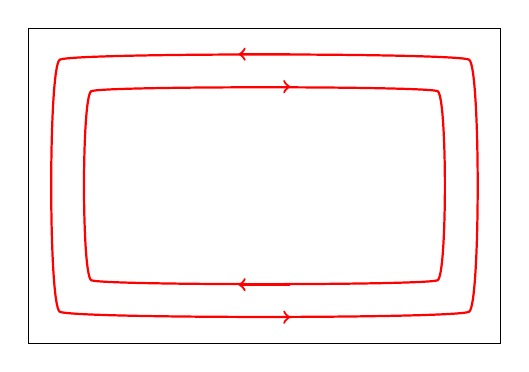
\begin{tikzpicture}
        \pgfmathsetmacro{\hL}{3};
        \pgfmathsetmacro{\vL}{2};
        \pgfmathsetmacro{\s}{0.4};
        \pgfmathsetmacro{\ss}{0.33};
        \draw (- \hL, - \vL) -- (- \hL, + \vL);
        \draw (- \hL, + \vL) -- (+ \hL, + \vL);
        \draw (+ \hL, + \vL) -- (+ \hL, - \vL);
        \draw (+ \hL, - \vL) -- (- \hL, - \vL);
        \draw [thick, red] plot [smooth cycle, tension=0.1] coordinates {(- \hL + 1*\s, - \vL+ 1*\s) (- \hL+ 1*\s, + \vL- 1*\s) (+ \hL- 1*\s, + \vL- 1*\s) (+ \hL- 1*\s, - \vL+ 1*\s)};
        \draw [thick, red, ->] (+1*\ss, + \vL - 1*\ss) -- (-1*\ss, + \vL - 1*\ss);
        \draw [thick, red, ->] (-1*\ss, - \vL + 1*\ss) -- (+1*\ss, - \vL + 1*\ss);
        \draw [thick, red] plot [smooth cycle, tension=0.1] coordinates {(- \hL + 2*\s, - \vL+ 2*\s) (- \hL+ 2*\s, + \vL- 2*\s) (+ \hL- 2*\s, + \vL- 2*\s) (+ \hL- 2*\s, - \vL+ 2*\s)};
        \draw [thick, red, ->] (-1*\ss, + \vL - 2.25*\ss) -- (+1*\ss, + \vL - 2.25*\ss);
        \draw [thick, red, ->] (+1*\ss, - \vL + 2.25*\ss) -- (-1*\ss, - \vL + 2.25*\ss);
    \end{tikzpicture}
\end{center}
This metal produces the \term{quantum spin hall effect}. We can define the current density $\ve j$,
\[ \ve j = - e n \ve v \]
Where $n$ is the density of the electrons which can be written as a integral over momentum space.
Doing so gives the current where the electrons move to the right as,
\[ I_R = - e \int v\tsb{F} n\tsb{F}\br{\vep_k} \f{\dif k_x}{2 \pi} \]
Where $k = 2\pi n / L$ and $2\pi / L$ is the volume in momentum space corresponding to a single quantum state.
\[ \f{1}{L} \f{\dif k_x}{\f{2 \pi }{L}} = \f{\dif k_x}{2 \pi} \]
If we convert this integral from an integral over momentum space to and integral over energies,
\[ \vep = \hbar v\tsb{F} k_x \implies \dif k_x = \f{\dif \vep}{\hbar v\tsb{F}} \]
Therefore the current is,
\[ I_{R} = - e v\tsb{F}  \f{1}{2\pi \hbar v\tsb{F}} \int_{-\inf}^{\vep_{FR}} \dif \vep = - \f{e}{h} \int_{-\inf}^{\vep_{FR}} \dif \vep \]
Where $\vep_{FR}$ is the Fermi energy for the right-traveling electrons.
The current for the electrons traveling to the left is opposite in sign,
\[ I_L = \f{e}{h} \int_{-\inf}^{\vep_{FL}} \dif \vep \]
Therefore the net current is,
\[ I = I_{R} + I_{L} = - \f{e}{h} \int_{\vep_{FL}}^{\vep_{FR}} \dif \vep = - \f{e}{h} \br{\vep_{FR} - \vep_{FL}} = - \f{e^2}{h} V_{y} \]
The conductivity is,
\[ \f{I}{V_{y}} = - \f{e^2}{h} \]
The interesting feature of this conductivity is that is only depends on the fundamental constants $e, h$. As it turns out, measurements of this conductivity represent our most precise measurements of $e$ and $h$. An excellent external resource is a book by R.B. Laughlin called \textit{Different Universe}. An important thing to remember that this analysis only applies for a particular spin value. In this case we analyzed spin up states $S^{z} = +1$. In general we have,
\[ \si_{xy}^{\uu} = -\f{e^2}{h} \qquad \si_{xy}^{\dd} = +\f{e^2}{h} \]
Which means that we can construct a \term{spin current},
\[ \si_{xy}^{S} =\f{1}{2} \br{\si_{xy}^{\uu} - \si_{xy}^{\dd}} = - \f{e^2}{h} \]
Effectively, if we have an equal number of electrons moving to the right and the left but each direction is biased to a particular spin, we can have a buildup of spin up electrons on the right and spin down electrons on the left. This is the analogue of \textit{spin voltage}. \\

\clearpage
\subsection{Bravais Lattices in 3D}

There are a number of typical Bravais lattices in three dimensions. The simplest one is the simple cubic.
\begin{enumerate}
    \item \term{Simple Cubic}:
    \begin{center}
        \begin{tikzpicture}
        \pgfmathsetmacro{\axissize}{1};
        \pgfmathsetmacro{\shiftx}{-4};
        \pgfmathsetmacro{\shifty}{0};
        \pgfmathsetmacro{\shiftz}{0};
        \draw[->] (\shiftx,\shifty, \shiftz) -- (\shiftx+\axissize,\shifty, \shiftz) node[right]{$y$};
        \draw[->] (\shiftx,\shifty, \shiftz) -- (\shiftx,\shifty+\axissize, \shiftz) node[above]{$z$};
        \draw[->] (\shiftx,\shifty, \shiftz) -- (\shiftx,\shifty, \shiftz+\axissize) node[below left]{$x$};
        \foreach \uda in {-1,+1}
        \foreach \udb in {-1,+1}
        \draw[gray, dashed]
        (-1,+\uda,+\udb) -- (+1,+\uda,+\udb)
        (+\uda,-1,+\udb) -- (+\uda,+1,+\udb)
        (+\uda,+\udb,-1) -- (+\uda,+\udb,+1)
        ;
        \foreach \x in {-1,+1}
        \foreach \y in {-1,+1}
        \foreach \z in {-1,+1}
        \draw[] (\x,\y,\z) node[fill=black, circle, inner sep=1pt]{};
        \draw[->] (-1,-1,-1) -- (+1,-1,-1) node[right]{$\ve a_2$};
        \draw[->] (-1,-1,-1) -- (-1,+1,-1) node[above]{$\ve a_3$};
        \draw[->] (-1,-1,-1) -- (-1,-1,+1) node[below left]{$\ve a_1$};
        \end{tikzpicture}
    \end{center}
    \[ \ve a_1 = a \hat x \quad \ve a_2 = a \hat y \quad \ve a_3 = a \hat z \]
    \item \term{Body-centered Cubic (bcc)}:
    \begin{center}
        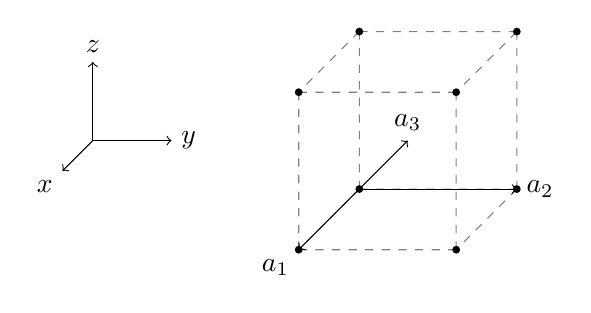
\begin{tikzpicture}
        \pgfmathsetmacro{\axissize}{1};
        \pgfmathsetmacro{\shiftx}{-4};
        \pgfmathsetmacro{\shifty}{0};
        \pgfmathsetmacro{\shiftz}{0};
        \draw[->] (\shiftx,\shifty, \shiftz) -- (\shiftx+\axissize,\shifty, \shiftz) node[right]{$y$};
        \draw[->] (\shiftx,\shifty, \shiftz) -- (\shiftx,\shifty+\axissize, \shiftz) node[above]{$z$};
        \draw[->] (\shiftx,\shifty, \shiftz) -- (\shiftx,\shifty, \shiftz+\axissize) node[below left]{$x$};
        \foreach \uda in {-1,+1}
        \foreach \udb in {-1,+1}
        \draw[gray, dashed]
        (-1,+\uda,+\udb) -- (+1,+\uda,+\udb)
        (+\uda,-1,+\udb) -- (+\uda,+1,+\udb)
        (+\uda,+\udb,-1) -- (+\uda,+\udb,+1)
        ;
        \foreach \x in {-1,+1}
        \foreach \y in {-1,+1}
        \foreach \z in {-1,+1}
        \draw[] (\x,\y,\z) node[fill=black, circle, inner sep=1pt]{};
        \draw[->] (-1,-1,-1) -- (+1,-1,-1) node[right]{$\ve a_2$};
        \draw[->] (-1,-1,-1) -- (0,0,0) node[above]{$\ve a_3$};
        \draw[->] (-1,-1,-1) -- (-1,-1,+1) node[below left]{$\ve a_1$};
        \end{tikzpicture}
    \end{center}
    \[ \ve a_1 = a \hat x \quad \ve a_2 = a \hat y \quad \ve a_3 = \f{a}{2}\br{\hat x + \hat y + \hat z} \]
    An alternative choice of primitive translation vectors that does not assign a bias to a particular vector is,
    \[ \ve a_1 = \f{a}{2}\br{-\hat x + \hat y + \hat z} \quad \ve a_2 = \f{a}{2}\br{\hat x - \hat y + \hat z} \quad \ve a_3 = \f{a}{2}\br{\hat x + \hat y - \hat z} \]
    \item \term{Face-centered Cubic (fcc)}:
    \begin{center}
        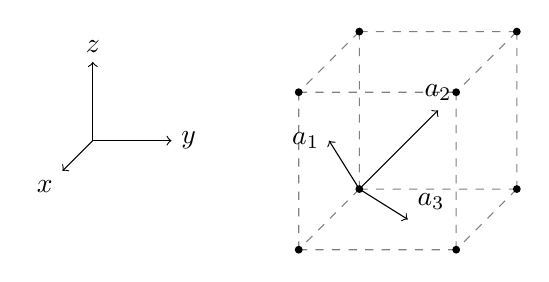
\begin{tikzpicture}
        \pgfmathsetmacro{\axissize}{1};
        \pgfmathsetmacro{\shiftx}{-4};
        \pgfmathsetmacro{\shifty}{0};
        \pgfmathsetmacro{\shiftz}{0};
        \draw[->] (\shiftx,\shifty, \shiftz) -- (\shiftx+\axissize,\shifty, \shiftz) node[right]{$y$};
        \draw[->] (\shiftx,\shifty, \shiftz) -- (\shiftx,\shifty+\axissize, \shiftz) node[above]{$z$};
        \draw[->] (\shiftx,\shifty, \shiftz) -- (\shiftx,\shifty, \shiftz+\axissize) node[below left]{$x$};
        \foreach \uda in {-1,+1}
        \foreach \udb in {-1,+1}
        \draw[gray, dashed]
        (-1,+\uda,+\udb) -- (+1,+\uda,+\udb)
        (+\uda,-1,+\udb) -- (+\uda,+1,+\udb)
        (+\uda,+\udb,-1) -- (+\uda,+\udb,+1)
        ;
        \foreach \x in {-1,+1}
        \foreach \y in {-1,+1}
        \foreach \z in {-1,+1}
        \draw[] (\x,\y,\z) node[fill=black, circle, inner sep=1pt]{};
        \draw[->] (-1,-1,-1) -- (-1,+0,+0) node[left]{$\ve a_1$};
        \draw[->] (-1,-1,-1) -- (+0,-1,+0) node[above right]{$\ve a_3$};
        \draw[->] (-1,-1,-1) -- (+0,+0,-1) node[above]{$\ve a_2$};
        \end{tikzpicture}
    \end{center}
    \[ \ve a_1 = \f{a}{2} \br{\hat y + \hat z} \quad \ve a_2 = \f{a}{2} \br{\hat x + \hat z} \quad \ve a_3 = \f{a}{2} \br{\hat x + \hat y} \]
    \item \term{Diamond Structure}: The diamond crystal structure consists of a fcc Bravais lattice with a $2$-atom basis,
    \begin{center}
        \begin{tikzpicture}[scale=2]
        \pgfmathsetmacro{\axissize}{0.5};
        \pgfmathsetmacro{\shiftx}{-3};
        \pgfmathsetmacro{\shifty}{0};
        \pgfmathsetmacro{\shiftz}{0};
        \draw[->] (\shiftx,\shifty, \shiftz) -- (\shiftx+\axissize,\shifty, \shiftz) node[right]{$y$};
        \draw[->] (\shiftx,\shifty, \shiftz) -- (\shiftx,\shifty+\axissize, \shiftz) node[above]{$z$};
        \draw[->] (\shiftx,\shifty, \shiftz) -- (\shiftx,\shifty, \shiftz+\axissize) node[below left]{$x$};
        \foreach \uda in {-1,+1}
        \foreach \udb in {-1,+1}
        \draw[gray, dashed]
        (-1,+\uda,+\udb) -- (+1,+\uda,+\udb)
        (+\uda,-1,+\udb) -- (+\uda,+1,+\udb)
        (+\uda,+\udb,-1) -- (+\uda,+\udb,+1)
        ;
        \foreach \x in {-1,+1}
        \foreach \y in {-1,+1}
        \foreach \z in {-1,+1}
        \draw[] (\x,\y,\z) node[fill=black, circle, inner sep=1pt]{};
        \draw[->] (-1,-1,-1) -- (-1,+0,+0) node[left]{$\ve a_1$};
        \draw[->] (-1,-1,-1) -- (+0,-1,+0) node[left]{$\ve a_3$};
        \draw[->] (-1,-1,-1) -- (+0,+0,-1) node[left]{$\ve a_2$};
        \draw[red, ->] (-1,+0,+0) -- ++ (0.6,0.6,0.6) node[above right]{$\ve r$};
        \draw[red, ->] (+0,-1,+0) -- ++ (0.6,0.6,0.6) node[above right]{$\ve r$};
        \draw[red, ->] (+0,+0,-1) -- ++ (0.6,0.6,0.6) node[above right]{$\ve r$};
        \end{tikzpicture}
    \end{center}
    \[ \hat r = \f{a}{4}\br{\hat x + \hat y + \hat z} \]
    \[ \ve a_1 = \f{a}{2} \br{\hat y + \hat z} \quad \ve a_2 = \f{a}{2} \br{\hat x + \hat z} \quad \ve a_3 = \f{a}{2} \br{\hat x + \hat y} \]
\end{enumerate}

The Diamond structure is a generalization of the graphene lattice in 3D. Many materials include C (diamond), Si, Ge and Sn crystallize in this diamond structure. The nearest-neighbor hopping Hamiltonian is as follows,
\[ H_1 = - \sum_{\ve R} \br{t \ket{\ve R, 1}\bra{\ve R, 2} + t \ket{\ve R + \ve a_1, 1}\bra{\ve R, 2} + t \ket{\ve R + \ve a_2, 1}\bra{\ve R, 2} + t \ket{\ve R + \ve a_3, 1} \bra{\ve R, 2} + \text{h.c.}} \eq \label{eq:diamond_H1}\]
While the second-nearest neighbor terms are numerous. In fact there are $24$ terms written below,
\begin{align*}
\eq \label{eq:diamond_H2}
\begin{split}
H_2
&= i \f{8 \De\tsb{SO}}{a^2} \sum_{\al \in \bc{1,2}}\sum_{\ve R} \bigg[\cdots \\
&\qquad \cdots + \ket{\ve R + \ve a_1,\al} \bra{\ve R, \al} \ve S \cdot \br{\ve r \times \ve a_1} + \cdots \\
&\qquad \cdots + \ket{\ve R + \ve a_2,\al} \bra{\ve R, \al} \ve S \cdot \br{\ve r \times \ve a_2} + \cdots \\
&\qquad \cdots + \ket{\ve R + \ve a_3,\al} \bra{\ve R, \al} \ve S \cdot \br{\ve r \times \ve a_3} + \cdots \\
&\qquad \cdots + \ket{\ve R + \ve a_2 - \ve a_1,\al} \bra{\ve R, \al} \ve S \cdot \br{\ve r - \ve a_1} \times \br{\ve r -\f{a}{2} \hat y} + \cdots \\
&\qquad \cdots + \ket{\ve R + \ve a_3 - \ve a_1,\al} \bra{\ve R, \al} \ve S \cdot \br{\ve r - \ve a_1} \times \br{\ve r -\f{a}{2} \hat z} + \cdots \\
&\qquad \cdots + \ket{\ve R + \ve a_2 - \ve a_3,\al} \bra{\ve R, \al} \ve S \cdot \br{\ve r - \ve a_3} \times \br{\ve r -\f{a}{2} \hat y} + \cdots \\
&\qquad \cdots + \text{h.c.} \bigg]
\end{split}
\end{align*}

We can explicitly calculate the cross products,
\begin{align*}
    \ve r \times \ve a_1 &= \f{a^2}{8}\br{\hat x + \hat y + \hat z} \times \br{\hat y + \hat z} = \f{a^2}{8} \br{\hat z - \hat y}\\
    \ve r \times \ve a_2 &= \f{a^2}{8}\br{\hat x + \hat y + \hat z} \times \br{\hat z + \hat x} = \f{a^2}{8} \br{\hat x - \hat z}\\
    \ve r \times \ve a_3 &= \f{a^2}{8}\br{\hat x + \hat y + \hat z} \times \br{\hat x + \hat y} = \f{a^2}{8} \br{\hat y - \hat x}\\
    \br{\ve r - \ve a_1} \times \br{\ve r - \f{a}{2} \hat y} &= \f{a^2}{16}\br{\hat x - \hat y - \hat z} \times \br{\hat x - \hat y + \hat z} = -\f{a^2}{8}\br{\hat x + \hat y} \\
    \br{\ve r - \ve a_1} \times \br{\ve r - \f{a}{2} \hat z} &= \f{a^2}{16}\br{\hat x - \hat y - \hat z} \times \br{\hat x + \hat y - \hat z} = +\f{a^2}{8}\br{\hat x + \hat z} \\
    \br{\ve r - \ve a_3} \times \br{\ve r - \f{a}{2} \hat y} &= \f{a^2}{16}\br{-\hat x - \hat y + \hat z} \times \br{\hat x - \hat y + \hat z} = +\f{a^2}{8}\br{\hat y + \hat z}
\end{align*}
Therefore \cref{eq:diamond_H2} becomes,
\begin{align*}
\eq \label{eq:diamond_H2_computed_cross_product}
\begin{split}
H_2
&= i \De\tsb{SO}\sum_{\al \in \bc{1,2}}\sum_{\ve R} \bigg[\cdots \\
&\qquad \cdots + \ket{\ve R + \ve a_1,\al} \bra{\ve R, \al} \br{S^z - S^y} + \cdots \\
&\qquad \cdots - \ket{\ve R + \ve a_2,\al} \bra{\ve R, \al} \br{-S^x + S^z} + \cdots \\
&\qquad \cdots + \ket{\ve R + \ve a_3,\al} \bra{\ve R, \al} \br{S^y - S^x} + \cdots \\
&\qquad \cdots - \ket{\ve R + \ve a_2 - \ve a_1,\al} \bra{\ve R, \al} \br{S^x + S^y} + \cdots \\
&\qquad \cdots + \ket{\ve R + \ve a_3 - \ve a_1,\al} \bra{\ve R, \al} \br{S^x + S^z} + \cdots \\
&\qquad \cdots + \ket{\ve R + \ve a_2 - \ve a_3,\al} \bra{\ve R, \al} \br{S^y + S^z} + \cdots \\
&\qquad \cdots + \text{h.c.} \bigg]
\end{split}
\end{align*}

The nearest neighbors Hamiltonian \cref{eq:diamond_H1} can be Fourier transformed and partially diagonalized,
\[ H_1 = - \sum_{\ve k}\bc{\ket{\ve k, 1}\bra{\ve k, 2} \br{\br{t + \de t} + t e^{-i \ve k \cdot \ve a_1} + t e^{-i\ve k\cdot \ve a_2} + t e^{-i\ve k \cdot \ve a_3}} + \text{h.c.}} \]
Similarly for \cref{eq:diamond_H2_computed_cross_product},

\begin{align*}
\eq \label{eq:diamond_H2_computed_cross_product_ft}
\begin{split}
H_2
&= i \De\tsb{SO}\sum_{\al \in \bc{1,2}}\sum_{\ve k} \ket{\ve k,\al} \bra{\ve k, \al} \bigg[\cdots \\
&\qquad \cdots + e^{-i \ve k \cdot \ve a_1} \br{S^z - S^y} + \cdots \\
&\qquad \cdots + e^{-i \ve k \cdot \ve a_2} \br{S^x - S^z} + \cdots \\
&\qquad \cdots + e^{-i \ve k \cdot \ve a_3} \br{S^y - S^x} + \cdots \\
&\qquad \cdots - e^{-i \ve k \cdot \br{\ve a_2 - \ve a_1}} \br{S^x + S^y} + \cdots \\
&\qquad \cdots + e^{-i \ve k \cdot \br{\ve a_3 - \ve a_1}} \br{S^x + S^z} + \cdots \\
&\qquad \cdots + e^{-i \ve k \cdot \br{\ve a_2 - \ve a_3}} \br{S^y + S^z} + \cdots \\
&\qquad \cdots + \text{h.c.} \bigg]
\end{split}
\end{align*}

Introducing pseudo-spin $\ve \si = \br{\si^x, \si^{y}, \si^{z}}$
\begin{align*}
\begin{split}
\si^x &= \begin{pmatrix} 0 & 1 \\ 1 & 0 \end{pmatrix} = \ket{1} \bra{2} + \ket{2} \bra{1} \\
\si^y &= \begin{pmatrix} 0 & -i \\ i & 0 \end{pmatrix} = -i\br{\ket{1} \bra{2} - \ket{2} \bra{1}} \\
\si^z &= \begin{pmatrix} 1 & 0 \\ 0 & -1 \end{pmatrix} = \ket{1} \bra{1} - \ket{2} \bra{2}
\end{split}
\end{align*}
The first and second nearest-neighbor Hamiltonian can be modeled when the tunneling amplitudes in \cref{eq:diamond_H1} are perturbed a small amount $t \mapsto t + \de t$ using the $5$-component vector $\ve d\br{\ve k} = \br{d_1\br{\ve k},d_2\br{\ve k},d_3\br{\ve k},d_4\br{\ve k},d_5\br{\ve k}}$,
\begin{align*}
    d_1\br{\ve k} &= - \br{t + \de t} - t \bs{\cos \ve k \cdot \ve a_1 + \cos \ve k \cdot \ve a_2 + \cos \ve k \cdot \ve a_3} \\
    d_2\br{\ve k} &= - t \bs{\sin \ve k \cdot \ve a_1 + \sin \ve k \cdot \ve a_2 + \sin \ve k \cdot \ve a_3} \\
    d_3\br{\ve k} &= \De\tsb{SO} \bs{\sin \ve k \cdot \ve a_2 - \sin \ve k \cdot \ve a_3 - \sin \ve k \cdot \br{\ve a_2 - \ve a_1} + \sin \ve k \cdot \br{\ve a_3 - \ve a_1}} \\
    d_4\br{\ve k} &= \De\tsb{SO} \bs{\sin \ve k \cdot \ve a_3 - \sin \ve k \cdot \ve a_1 + \sin \ve k \cdot \br{\ve a_1 - \ve a_2} - \sin \ve k \cdot \br{\ve a_3 - \ve a_2}} \\
    d_5\br{\ve k} &= \De\tsb{SO} \bs{\sin \ve k \cdot \ve a_1 - \sin \ve k \cdot \ve a_2 - \sin \ve k \cdot \br{\ve a_1 - \ve a_3} + \sin \ve k \cdot \br{\ve a_2 - \ve a_3}}
\end{align*}
Using this the full Hamiltonian can be written as,
\[ H\br{\ve k} = d_1\br{\ve k} \si^x + d_2\br{\ve k}  \si^y  + d_3\br{\ve k} \si^{z}S^x + d_4\br{\ve k} \si^z S^y + d_5\br{\ve k}\si^zS^z \]
Where the matrices on the right of each $d_i\br{\ve k}$ term are the usual $4 \time 4$ gamma matrices $\ga^{\mu}$ from the Dirac equation.
\[ \ga^{0} = \si^{x} \quad \ga^{0}\ga^{1} = \si^{y} \quad \ga^{0}\ga^{2} = \si^{z}S^{x} \quad \ga^{0}\ga^{3} = \si^{z}S^y \quad \ga^{0}\ga^{5} = \si^{z} S^{z}\]
\[ \ga^{1} = \si^{x} \si^{y} = i \si^z \quad \ga^{2} = i \si^{y}S^{x} \ga^{3} = i \si^{y}S^{y} \]
\[ i \ga^{0}\ga^{1}\ga^{2}\ga^{3} = i \si^{x} i \si^{z} i \si^{y}S^{x} = \si^{y}S^{z} \defined \ga^{5} \]
It is convenient to rename these matrices using capital gammas,
\begin{alignat*}{2}
\Ga^{1} &= \ga^{0} &= \si^{x} \\
\Ga^{2} &= \ga^{0}\ga^{1} &= \si^{y} \\
\Ga^{3} &= \ga^{0}\ga^{2} &= \si^{z}S^{x} \\
\Ga^{4} &= \ga^{0}\ga^{3} &= \si^{z}S^y \\
\Ga^{4} &= \ga^{0}\ga^{5} &= \si^{z} S^{z}
\end{alignat*}
It is easy to see that these $\Ga$ matrices obey the \term{Clifford Algebra},
\[ \bc{\Ga^{a}, \Ga^{b}} = 2 \de_{ab} \]
Thus we have that,
\[ H\br{\ve k} = \sum_{a = 1}^{5} d_a\br{\ve k}\Ga^{a} \defined d_a\br{\ve k}\Ga^{a} \eq \label{eq:HGa}\]
Just like in graphene, we see that the parity transformation $P = \si^{x} = \ga^{0}$ leaves $\Ga^{1}$ even under parity and $\Ga^{2,3,4,5}$ odd under parity. One reason motivating why we should write \cref{eq:HGa} in terms of the $\Ga$ matrices is that we can now easily find the eigenvalues by squaring the Hamiltonian,
\[ H^2\br{\ve k} = d_a\br{\ve k}\Ga^{a} d_b\br{\ve k}\Ga^{b} = d_a \br{\ve k} d_a\br{\ve k} \]
Therefore,
\[ \vep_{\pm}\br{\ve k} = \pm \sqrt{d_a \br{\ve k} d_a\br{\ve k}} = \pm \abs{\ve d\br{\ve k}} \]
We now elect to compute the reciprocal basis vectors. Recall that,
\[ \ve a_1 = \f{a}{2} \br{\hat y + \hat z} \quad \ve a_2 = \f{a}{2} \br{\hat x + \hat z} \quad \ve a_3 = \f{a}{2} \br{\hat x + \hat y} \]
Define the scalar $v_c$ such that,
\[ v_c = \ve a_1 \cdot \br{\ve a_2 \times \ve a_3} = \cdots = \f{a^3}{4} \]
The reciprocal vectors become,
\[ \ve b_1 = \f{2\pi}{v_c} \ve a_2 \times \ve a_3 = \f{2 \pi}{a} \br{\hat y - \hat x + \hat z} \]
Similarly,
\[ \ve b_2 = \f{2\pi}{v_c} \br{\hat z - \hat y + \hat x} \]
\[ \ve b_3 = \f{2\pi}{v_c} \br{\hat x - \hat z + \hat y} \]
Therefore the reciprocal lattice of fcc is the bcc lattice vectors and vice versa.
When $\de t = 0$ the $5$-component $\ve d\br{\ve k}$ vanishes at $3$ inequivalent band-touching point in the first Brillouin zone.
\[ X^{x} = \f{2\pi}{a}\br{1,0,0} \qquad X^{y} = \f{2\pi}{a}\br{0,1,0} \qquad X^{z} = \f{2\pi}{a}\br{0,0,1} \]
Considering the $X^{z}$ point as an illustrative example we have $k_1 = k_2 = \f12$ and $k_3 = 0$. If we expand in small deviations from the $X^z$ point where $\ve k \simeq X^{z} + \ve q = \br{q_x, q_y, \f{2\pi}{a} + q_z}$ we obtain the following,
\begin{align*}
    d_1\br{\ve k} &\simeq -t - \de t - t \br{-1} = - \de t \\
    d_2\br{\ve k} &\simeq t a q_z \\
    d_3\br{\ve k} &\simeq -2\De\tsb{SO} a q_x \\
    d_4\br{\ve k} &\simeq 2\De\tsb{SO} a q_y \\
    d_5\br{\ve k} &\simeq \f{\De\tsb{SO}}{8} a^3 \br{q_y^2 - q_x^2} q_z
\end{align*}
Thus we obtain (replacing $\ve q$ with $\ve k$ again),
\[ H_{X^{z}} = - \de t \si^{x} + t a k_z \si^{y} - 2 \De\tsb{SO} a \si^{z} S^{x} k_x + 2 \De\tsb{SO} a \si^{z} S^{y} k_y \]
Analogously expanding about $X^{y}$ and $X^{x}$,
\[ H_{X^{y}} = - \de t \si^{x} + t a k_y \si^{y} + 2 \De\tsb{SO} a k_x \si^{z} S^{x} - 2 \De\tsb{SO} a k_z \si^{z} S^{z} \]
\[ H_{X^{x}} = - \de t \si^{x} + t a k_x \si^{y} - 2 \De\tsb{SO} a k_y \si^{z} S^{y} + 2 \De\tsb{SO} a k_z \si^{z} S^{z} \]
Notice that $H_{X^{x,y,z}}$ look like anisotropic Dirac Hamiltonians where $\de t$ plays the role of the Dirac mass.
\[ \vep_{\pm}\br{\ve k} = \pm \sqrt{t^2 a^2 k_z^2 + 4 \De\tsb{SO}^2 a^2 \br{k_x^2 + k_y^2} + \de t^2} \]
Changing the sign of $\de t$ corresponds to transitions between topological and ordinary insulators.
\begin{itemize}
    \item $\de t > 0$: topological
    \item $\de t < 0$: ordinary
    \item $\de t = 0$: Dirac semimetal
\end{itemize}

\subsection{Quantum Hall Effect}

In this subsection we will discuss the Quantum Hall Effect. Specifically we will look at the Quantum Hall Effect in a $2$-dimensional electron gas (2DEG) when subjected to a magnetic field. 2DEG arise at heterointerfaces; interfaces between two different semiconductor materials. Semiconductors are insulators with a small band gap $<\SI{1}{\eV}$.

\begin{center}
\begin{tikzpicture}
    \draw (-3, 3) node[]{$\text{Al}_{x} \text{Ga}_{1-x} \text{As}$};
    \draw (+3, 3) node[]{$\text{GaAs}$};
    \draw (0, -3) -- (0, 3);
    \draw[dashed] (-4, 1) -- (+4, 1) node[right]{$\vep\tsb{F}$};
    \draw [] plot [smooth, tension=1] coordinates {(-4, 1.5) (-1, 1.8) (0, 2.5)};
    \draw [] plot [smooth, tension=1] coordinates {(+4, 1.5) (+1, 1.2) (0, 0.5)};
    \draw [] plot [smooth, tension=1] coordinates {(-4, -2.5) (-1, -2.2) (0, -1.5)};
    \draw [] plot [smooth, tension=1] coordinates {(+4, -0.5) (+1, -0.8) (0, -1.5)};
\end{tikzpicture}
\end{center}

Modeling a 2DEG corresponds to subjecting the electrons in state $\ket{\psi}$ to a potential $V\br{\ve r}$ and making use of the Schrödinger equation,
\[ \br{-\f{\hbar^2}{2m} \del^2 + V\br{\ve r}}\psi\br{\ve r} = E \psi\br{\ve r} \eq \label{eq:tise} \]
Where $\psi\br{\ve r} \defined \braket{\ve r}{\psi}$ is the position space wavefunction. In order to model electrons confined to two dimensions (say $x,y$) use the following potential,
\[ V\br{\ve r} = \begin{cases}
    0 & \ve r \cdot \hat z = 0 \\
    \inf & \ve r \cdot \hat z \neq 0
\end{cases} \eq \label{eq:potential}\]
By doing so, $\psi\br{\ve r}$ is confined to be non-zero within the $xy$-plane.
\[ \psi\br{\ve r} = \psi\br{x \hat x + y \hat y } \defined \psi\br{x,y} \]
Furthermore let $L_x$ and $L_y$ denote the side lengths of rectangle space accessible by the electrons equipped with periodic boundary conditions,
\[ \psi\br{x + L_x, y} = \psi\br{x, y+ L_y} = \psi\br{x,y} \eq \label{eq:boundary_conditions} \]
The electrons inside the accessible region are subject to no external potential. Therefore the electrons will exhibit plane-wave behaviour with $z = 0$.
\[ \psi\br{\ve r} = \ga e^{i \ve k \cdot \ve r} = \ga e^{i \br{k_x x + k_y y}} \eq \label{eq:2dansatz} \]
Where $\ve k = k_x \hat x + k_y \hat y$ denotes the momentum wave vector of the electron and $\ga \in \R$ is a normalization factor. The normalization factor comes from the desired normalization of the state $\psi\br{\ve r}$,
\[ 1 = \braket{\psi}{\psi} = \intl_{0}^{L_x} \dif x \intl_{0}^{L_y} \dif y \braket{\psi}{\ve r}\braket{\ve r}{\psi} = \intl_{0}^{L_x} \dif x \intl_{0}^{L_y} \dif y \ga^2 \abs{e^{i \br{k_x x + k_y y}}}^2 = L_x L_y \ga^2 \]
Therefore the normalization is simply,
\[ \ga = \f{1}{\sqrt{L_x L_y}} \]
Consequently \cref{eq:2dansatz} becomes,
\[ \psi\br{\ve r} = \f{1}{\sqrt{L_x L_y}} e^{i \br{k_x x + k_y y}} \]
Moreover the boundary conditions \cref{eq:boundary_conditions} quantize the accessible values of $k_x, k_y$,
\[ e^{i \br{k_x\br{x + L_x} + k_y y}} = e^{i \br{k_x x + k_y \br{y + L_y}}} = e^{i \br{k_x x + k_y y}} \]
\[ e^{i k_x L_x} = e^{i k_y L_y} = 1 \implies k_x = \f{2 \pi m_x}{L_x} \quad k_y = \f{2 \pi m_y}{L_y} \quad m_x, m_y \in \bc{0, \pm 1, \pm 2,\ldots} \]
Therefore the accessible points in $k$-space form a square lattice which is illustrated below,
\begin{center}
    \begin{tikzpicture}
        \pgfmathsetmacro{\plotsize}{4};
        \pgfmathsetmacro{\ll}{0.6};
        \pgfmathsetmacro{\count}{5};
        \pgfmathsetmacro{\shift}{0.3};

        \draw[thick, ->] (-\plotsize, +0) -- (+\plotsize, +0) node[right]{$k_x$};
        \draw[thick, ->] (+0, -\plotsize) -- (+0, +\plotsize) node[above]{$k_y$};

        \foreach \x in {-\count,...,\count}{
            \foreach \y in {-\count,...,\count}{
                \draw (\ll*\x, \ll*\y) node[circle, inner sep=1pt, fill=red](\x d \y){};
            }
        }

        \draw[|<->|] ($\ll*(-5,-5) + (0,-\shift)$) -- node[below]{$\f{2\pi}{L_x}$} ($\ll*(-4,-5) + (0,-\shift)$);
        \draw[|<->|] ($\ll*(-5,-5) + (-\shift,0)$) -- node[left ]{$\f{2\pi}{L_y}$} ($\ll*(-5,-4) + (-\shift,0)$);

        \draw[blue, fill=blue, fill opacity=0.2] (3*\ll,3*\ll) +(-\ll/2,-\ll/2) rectangle +(+\ll/2,+\ll/2);
        \draw[green, fill=green, fill opacity=0.2] (0,0) circle (2);
        \draw[->] (0,0) -- node[below]{$k$} ({sqrt(2)},{sqrt(2)});
    \end{tikzpicture}
\end{center}
Clearly, each accessible momentum state occupies an area (shaded in blue) equal to,
\[ \br{\f{2\pi}{L_x}}\br{\f{2\pi}{L_y}} = \f{\br{2 \pi}^2}{\s A} \]
Where $\s A = L_x L_y$ is the total area. In the inverse of this statement is that there are,
\[ \f{\s A}{\br{2\pi}^2} \eq \label{eq:area}\]
grid points per unit area of $k$-space. Using \cref{eq:tise}, we can now calculate the energy for the state $\psi\br{r_x, r_y} \defined \braket{\ve r}{\psi}$.
\[ E \psi \br{\ve r} = -\f{\hbar^2}{2m} \del^2 \psi\br{\ve r} = -\f{\hbar^2}{2m} \br{\di_x^2 + \di_y^2} \psi\br{\ve r} = -\f{\hbar^2}{2m} \br{-k_x^2 -k_y^2} \psi\br{\ve r} = \f{\hbar^2}{2m} k^2 \psi\br{\ve r}\]
Where $k = \sqrt{k_x^2 + k_y^2}$ is a radius in $k$-space. Therefore the energy levels are,
\[ E = \f{\hbar^2 k^2}{2m} = \f{\hbar^2}{2m}\br{2\pi}^2 \br{\f{m_x^2}{L_x^2} + \f{m_y^2}{L_y^2}} \qquad m_x, m_y \in \bc{0, \pm1, \pm2, \ldots} \eq \label{eq:energy_levels}\]
Let $N\br{\vep}$ denote the number of states accessible to a single electron with energy $\vep$. Since this function is generally non-trivial, we approximate $N\br{\vep}$ as the infinitesimal amount $\de N\br{\vep}$ as follows,
\[ \de N\br{\vep} \simeq N_{<} \br{\vep + \de \vep/2} - N_{<} \br{\vep - \de \vep/2} \]
Where $N_{<}\br{\vep}$ is the number of states accessible to any electron with at most energy $\vep$. Evidently this quantity is proportional to an area in $k$-space. Namely, the area of $k$ space associated with $N_{<}$ is a circle centered at $\br{k_x, k_y} = \br{0,0}$. Therefore,
\[ N_{<}\br{\vep} \propto \pi k^2 = \pi \f{2m \vep}{\hbar^2} \]
The proportionality constant is exactly \cref{eq:area},
\[ N_{<}\br{\vep} = \f{\s A}{\br{2\pi}^2} \f{2m\pi  \vep}{\hbar^2} \]
Therefore,
\[ \de N\br{\vep} = \f{\s A}{\br{2\pi}^2} \f{2m\pi}{\hbar^2} \de \vep \]
Forming a differential form,
\[ \der{N}{\vep} = \f{\s A}{\br{2\pi}^2} \f{2m\pi}{\hbar^2} \]
The density of states is a constant. Normalizing for area,
\[ \f{1}{\s A}\der{N}{\vep} = \f{2m\pi}{\br{2\pi}^2\hbar^2} \]
This however, does not account for the fact that each electron has two accessible spin states for each $k$-space lattice point. Therefore, there are truly twice as many states available to each electron,
\[ \f{1}{\s A}\der{N}{\vep} = \f{4m\pi}{\br{2\pi}^2\hbar^2} \]
Therefore the density of states is,
\[ g\br{\vep} \defined \f{1}{\s A}\der{N}{\vep} = \f{m}{\pi \hbar^2} \eq \label{eq:2d_density_of_states} \]
The electron density for a given Fermi wavevector $k\tsb{F}$ is the number of electrons per unit area in $r$-space. At zero temperature and Fermi energy $\vep\tsb{F}$ the states in $k$-space are occupied at lowest energies first. Therefore the total number of electrons $N\br{\vep\tsb{F}}$ is given by,
\[ N\br{\vep\tsb{F}} = \s A\int_{0}^{\vep\tsb{F}} \dif \vep g\br{\vep} = \s A \int_{0}^{\vep\tsb{F}} \dif \vep \f{m}{\pi \hbar^2} = \f{m}{\pi \hbar^2} \vep\tsb{F} \s A \]
Given that the Fermi energy and Fermi wavevector are related via \cref{eq:energy_levels}, the electron density is,
\[ n\br{k\tsb{F}} = \f{1}{\s A} N\br{k\tsb{F}} = \f{m}{\pi \hbar^2} \f{\hbar^2 k\tsb{F}^2}{2m} \]
\[ n\br{k\tsb{F}} = \f{k\tsb{F}^2}{2\pi} \eq \label{eq:electron_density}\]

Now, we place the 2DEG in the $xy$-plane and subject it to a magnetic field in the $z$-direction $\ve B = B \hat z$. If the electrons are classical particles of charge $-e$ and mass $m$,
\[ \der{\ve p}{t} = \ve F\tsb{L} = - \f{e}{c}\ve v \times \ve B \qquad \ve v = \f{\ve p}{m}, \ve v = \der{\ve r}{t} \]
Solving these equations yields,
\[ m \dder{\ve r}{t} = - \f{e}{c} \der{\ve r}{t} \times \ve B  \]
Therefore we obtain a two dimensional system of coupled ordinary differentiable equations,
\begin{align*}
\dder{x}{t} &= - \f{eB}{mc} \der{y}{t} \\
\dder{y}{t} &= \f{eB}{mc} \der{x}{t}
\end{align*}
Where the frequency $\w_c = \f{eB}{mc}$ is the cyclotron frequency. In order to solve this system, introduce a complex parameter $z = x + i y$ such that,
\[ \dder{x}{t} = i \w_x \der{z}{t} \]
\[ z\br{t} = z_0 - \f{i v_0}{\w_c}e^{i \w_c t}  \]
Which is circular motion with frequency $\w_c$. Therefore if we need to model the average time between collisions with impurities, the simplest description involves a decrease in momentum with characteristic time $\tau$.
\[ \der{\ve p}{t} = - e \br{\ve E + \f{1}{c} \ve v \times \ve B} - \f{\ve p}{\tau} \]
Therefore without a magnetic field we have,
\[ \der{\ve p}{t} = \f{- \ve p}{\tau} \implies \ve p\br{t} = \ve p\br{0} e^{- t/\tau} \]
In general,
\[ m\der{\ve v}{t} = - \f{m \ve v}{\tau} - e\br{\ve E + \f{1}{c} \ve v \times \ve B} \]
Assuming that $\ve E$ and $\ve B$ are time-independent, we can look for the time-independent steady state solution corresponds to a fixed $\ve v$,
\[ \der{\ve v}{t} = 0 \implies \ve v  -\f{e \tau}{m} \br{\ve E + \f{1}{c} \ve v \times \ve B} \]
The electron $\ve v$ is connect to the current density $\ve j$ through the following equation we have seen before,
\[ \ve j = - e n \ve v \]
Where $n$ is the electron density and $e$ is the electric charge. Therefore,
\[ \ve j = \f{e^2 n \tau}{m} \br{\ve E - \f{e \tau}{m c} \ve j \times \ve B} \]
In the absence of a magnetic field $\ve B$, we recover Ohm's law,
\[ \ve j = \f{e^2 n \tau}{m} \ve E \]
Where the proportionality is the conductivity $\si$,
\[ \si = \f{e^2 n \tau}{m} \]
The electric field is,
\[ \ve E = \f{\ve j}{\si} - \f{1}{nec} \ve B \times \ve j \]
Component-wise,
\begin{align*}
    E_x &= \f{1}{\si} j_x + \f{B}{nec} j_y \\
    E_y &= \f{1}{\si} j_y - \f{B}{nec} j_x
\end{align*}
If there is no current in the $y$-direction ($j_y = 0$) we have,
\[ E_y = -\f{B}{nec} j_x \qquad \f{E_y}{B j_x} = -\f{1}{nec} = - R_H \]
The last equality is a definition of the \term{Hall coefficient} $R_H$
\[ R_H = \f{1}{nec} \]
Notice that the Hall coefficient only depends on the density of the electrons and other fundamental constants. Now we introduce the \term{resistivity tensor},
\[\rho = \begin{pmatrix}
    1 / \si & B R_{H} \\
    -B R_{H} & 1 / \si \\
\end{pmatrix} \]
We refer to this as the \term{classical Hall effect}.

\begin{center}
\begin{tikzpicture}
    \pgfmathsetmacro{\axissize}{4};
    \pgfmathsetmacro{\plotsize}{4};
    \draw[->] (0,0) -- (+\axissize,0) node[right]{$B$};
    \draw[->] (0, 0) -- (0,+\axissize) node[above]{$\rho_{xy}$};
    \draw[red] (1, 0) arc (0:27:1) node[midway, right]{$R_{H}$};
    \draw[scale=1.0,domain=0:\plotsize,smooth,variable=\B,red] plot ({\B},{0.5*\B});
\end{tikzpicture}
\end{center}

In reality, the classical Hall effect occurs at weak magnetic fields or in dirty samples.
If we let $1/\tau$ characterize the impurity scattering rate, our classical Hall effect is relevant in the domain where,
\[ \w_{C} \tau \ll 1 \]
Recall that the cyclotron frequency is $\w_c$,
\[ \w_c = \f{eB}{mc} \]
If $\w_{C} \tau \ll 1$, the electron will be scatter many times before being able to complete a single circular orbit; i.e. if the period of the circular motion of the electron is greater than the mean-free time, then we can model the electrons as a classical particle.\\

In we have $\w_{C} \tau \gg 1$, then the classical Hall effect is no longer the dominant feature. If the circular motion of the electrons becomes quantized, we need to consider the \term{quantum Hall effect}. The quantum aspects of the electron need to be considered in really clean materials or in high magnetic fields.\\

To study the quantum Hall effect, consider free quantum particles of charge $-e$ in the $xy$-plane in a magnetic field $\ve B= B \hat z$ pointing in the $\hat z$ direction. In the absence of a magnetic field, we have the relation $\ve p = m \ve v$ which makes the Hamiltonian,
\[  H = - \f{\hbar^2 \del^2}{2m} \]
However, a magnetic field $\ve B = \vdel \times \ve A$ we have,
\[ m \ve v = \ve p + \f{e}{c} \ve A \]
Therefore the Hamiltonian for a charged particle in a magnetic field is,
\[ H = \f{1}{2m} \br{- i \hbar \vdel + \f{e}{c} \ve A}^2 - \ve \mu \cdot \ve B \]
Where $\ve \mu$ is the magnetic dipole moment. For simplicity, we neglect $\ve \mu$ for now. Therefore, the Hamiltonian of interest is,
\[ H = \f{1}{2m} \br{- i \hbar \vdel + \f{e}{c} \ve A}^2 \eq \label{eq:quantum_hall_ham} \]
Where we wish to find the energy eigenstates $\psi$ where $H \psi = E \psi$. Moreover, the magnetic field is determined by $\ve B = \vdel \times \ve A$ leaving a \term{gauge invariance} in the choice of $\ve A$,
\[ \ve A \to \ve A + \vdel f \]
The gauge choice we will used is called the \term{Landau gauge}.
\[ \ve A = x B \hat y \]
Therefore,
\[ \br{\vdel \times \ve A}_{z} = \pder{A_y}{x} - \pder{A_x}{y} = B \]
Analogously the $x,y$ components of $\vdel \times \ve A$ are as follows,
\[ \br{\vdel \times \ve A}_{x} = \pder{A_z}{y} - \pder{A_y}{z} = 0 \]
\[ \br{\vdel \times \ve A}_{y} = \pder{A_x}{z} - \pder{A_z}{x} = 0 \]
Therefore \cref{eq:quantum_hall_ham} becomes,
\begin{align*}
    H
    &= \f{1}{2m}\br{- i \hbar \vdel + \f{e}{c} \ve A}^2 \\
    &= \f{1}{2m}\br{- i \hbar \vdel + \f{e\ve B}{c} \times \hat y}^2 \\
    &= - \f{\hbar^2}{2m} \pdder{}{x} + \f{1}{2m}\br{- i \hbar \pder{}{y} + \f{eB}{c}x}^2 \eq \label{eq:quantum_hall_ham_landau}
\end{align*}
Notice that $H$ is not invariant with respect to translations along the $x$-direction but \textit{is} invariant with respect to translations along the $y$-direction. Translation symmetries give rise to wave functions that are also momentum eigenstates. If the energy eigenstates $\psi\br{x,y}$ are thus functions of $x,y$ and have the following form,
\[ H \psi\br{x,y} = E \psi\br{x,y} \]
Symmetry analysis suggests we should expect $\psi$ to the separable into a plane wave solution with non-trivial $x$-dependence $\vp\br{x}$.
\[ \psi\br{x,y} = e^{i k_y y} \vp\br{x} \]
With $k_y$ to be determined. Substituting this ansatz into \cref{eq:quantum_hall_ham_landau} yields,
\[ E \psi\br{x,y}= - \f{\hbar^2}{2m} \pdder{\vp}{x} e^{ik_yy} + \f{1}{2m}\br{\hbar k_y + \f{eB}{c}x}^2 \vp e^{ik_yy} \]
Canceling $\vp$,
\[ E \vp = - \f{\hbar^2}{2m} \pdder{\vp}{x} + \f{1}{2m}\br{\hbar k_y + \f{eB}{c}x}^2 \vp \eq \label{eq:hall1D}\]
Gives us a 1D differential equation. For convenience of notation we introduce the \term{magnetic length} $\ell$,
\[ \ell = \sqrt{\f{\hbar c}{eB}} \]
Additionally re-use the classical cyclotron frequency,
\[ \w_{C} = \f{eB}{mc} \]
Using these constants, \cref{eq:hall1D} can we re-expressed as,
\[ -\f{\hbar^2}{2m} \pdder{\vp}{x} + \f{m\w_{C}^2}{2} \br{x + k_y \ell^{2}}^2 \vp = E \vp \]
At this stage, it should be clear that this Hamiltonian is nothing more than a 1D Harmonic oscillator with frequency $\w_{C}$ and centered at $x = - k_y \ell^{2}$. The solution for the quantum harmonic oscillator can be found in a number of undergraduate quantum theory textbooks.
\[ \psi_{n k_y}\br{x} = \f{e^{ik_y y}}{\sqrt{\ell \sqrt{\pi} 2^{n} n!}} e^{-\f{1}{2 \ell^2} \br{x + k_y \ell^2}^2} H_n\br{\f{x + k_y \ell^2}{\ell}} \]
Where $H_n$ is the \term{$n$-th Hermite polynomial}. The wave function solutions are given by the Hermite polynomials, but the important feature are the quantized energy levels,
\[ E_{n,k_y} = \hbar \w_c \br{n + \f12} \qquad n \in \bc{0, 1, 2, \ldots} \]
Where $n$ are referred to as the Landau levels. This energy level is completely independent of $k_y$ but $k_y$ is independently quantized like a particle in a periodic potential,
\[ k_y = \f{2\pi}{L_y} m_y \qquad m_y \in \bc{0, \pm 1, \pm 2, \ldots}\]
Since the effective harmonic oscillator is centered at $-k_y \ell^2$, it must be that $L_x$ is twice the position of $k_y \ell^2$,
\[ -L_x \leq -k_y \ell^2 \leq 0 \implies 0 \leq k_y \leq \f{L_x}{\ell^2} \]
Therefore the total number of states for a fixed Landau level $n \in \bc{0,1,2,\ldots}$ is given by the $m_y$ value such that $k_y$ is bounded by $L_x / \ell^2$,
\[ N_{\phi} = \max{m_y} = \max{k_y} \f{L_y}{2\pi} = \f{L_yL_x}{2\pi\ell^2} = \f{L_xL_y eB}{2 \pi \hbar c}  \eq \label{eq:landau_occupancy}\]
Which is independent of $n$. Therefore, the number of electrons in each Landau level is the same for each Landau level. The density of states $g\br{\vep}$ forms a Dirac comb structure. In reality, however, the uncertainty principle smooths this plot due to uncertainty broadening. For low scattering rates (pure materials) we have the following profile.
\begin{center}
    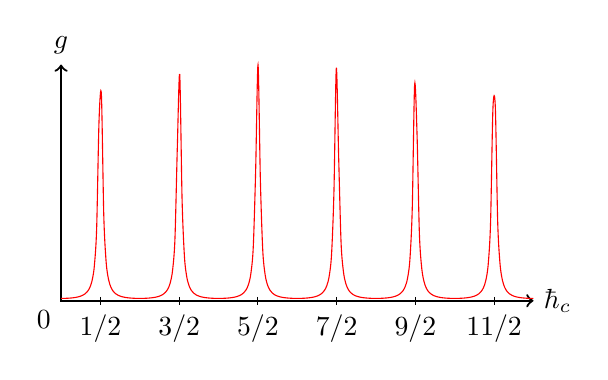
\begin{tikzpicture}
        \draw[thick, <->] (0, 3) node[above]{$g\br{\vep}$} -- (0,0) node[below left]{$0$} -- (6,0) node[right]{$\f{\vep}{\hbar \w_c}$};
        \draw[red, samples=200,smooth, domain=0:6, variable=\e] plot ({\e}, {0.03/((cos(deg(pi*\e)))^2 + 0.01)});
        \foreach \x in {1,3,5,7,9,11}{
            \draw ({\x/8*4}, +0.05) -- ({\x/8*4}, -0.05) node[below]{$\x/2$};
        }
    \end{tikzpicture}
\end{center}
Broadening increases due to impurities for the following reason. Suppose that an electron exists in a quantum state for some time $\tau$ which corresponds to the mean free time between collisions. The uncertainty in energy time is,
\[ \De \vep \De t \sim \De \vep \tau \sim \hbar \implies \De \vep \sim \f{\hbar}{\tau} \]
In regimes where $\tau$ is very small, the broadening results in the following,
\begin{center}
    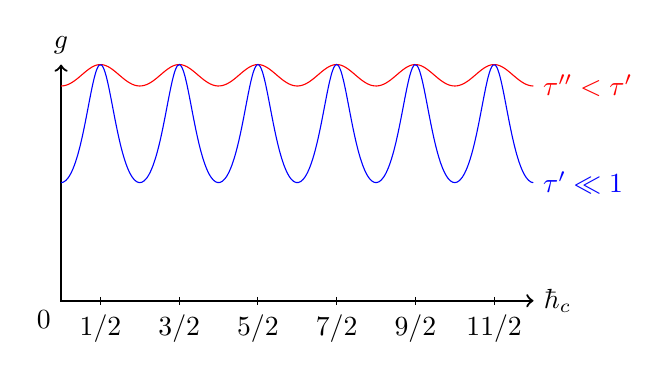
\begin{tikzpicture}
        \draw[thick, <->] (0, 3) node[above]{$g\br{\vep}$} -- (0,0) node[below left]{$0$} -- (6,0) node[right]{$\f{\vep}{\hbar \w_c}$};
        \draw[red, samples=200,smooth, domain=0:6, variable=\e] plot ({\e}, {30/((cos(deg(pi*\e)))^2 + 10)})node[right]{$\tau'' < \tau'$};
        \draw[blue, samples=200,smooth, domain=0:6, variable=\e] plot ({\e}, {3/((cos(deg(pi*\e)))^2 + 1)}) node[right]{$\tau' \ll 1$};
        \foreach \x in {1,3,5,7,9,11}{
            \draw ({\x/8*4}, +0.05) -- ({\x/8*4}, -0.05) node[below]{$\x/2$};
        }
    \end{tikzpicture}
\end{center}
Which more closely approximates the classical regime when $\w_c \tau \ll 1$ and the density $g\br{\vep}$ becomes more uniform.
\[ g\br{\vep} \approx g_0 = \f{m}{\pi \hbar^2} \]
Which is identically the 2D electron density of states in the absence of a magnetic field \cref{eq:2d_density_of_states}.\\

We refer to these energy levels as \term{Landau levels}. Every Landau level is degenerate with respect to all the different values of $k$. Since $E_{nk}$ is independent of $k$, we say that $E_{nk}$ has degeneracies in $k$. Because of this, Landau levels are analogous to bands in a crystal. \\

An alternative interpretation of \cref{eq:landau_occupancy} is to define the following: The total magnetic flux through the sample area $B L_x L_ y \defined \phi$ and the magnetic flux quantum $hc / e \defined \phi_0$. Then the Landau occupancy number becomes a flux ratio,
\[ N_{\phi} = \f{\phi}{\phi_0} \]

Combining the Landau level description at high magnetic fields $B$ gives a completely new description of the resistivity $\rho_{xy}$ and $\rho_{xx}$,

\begin{center}
    \hspace*{+3em}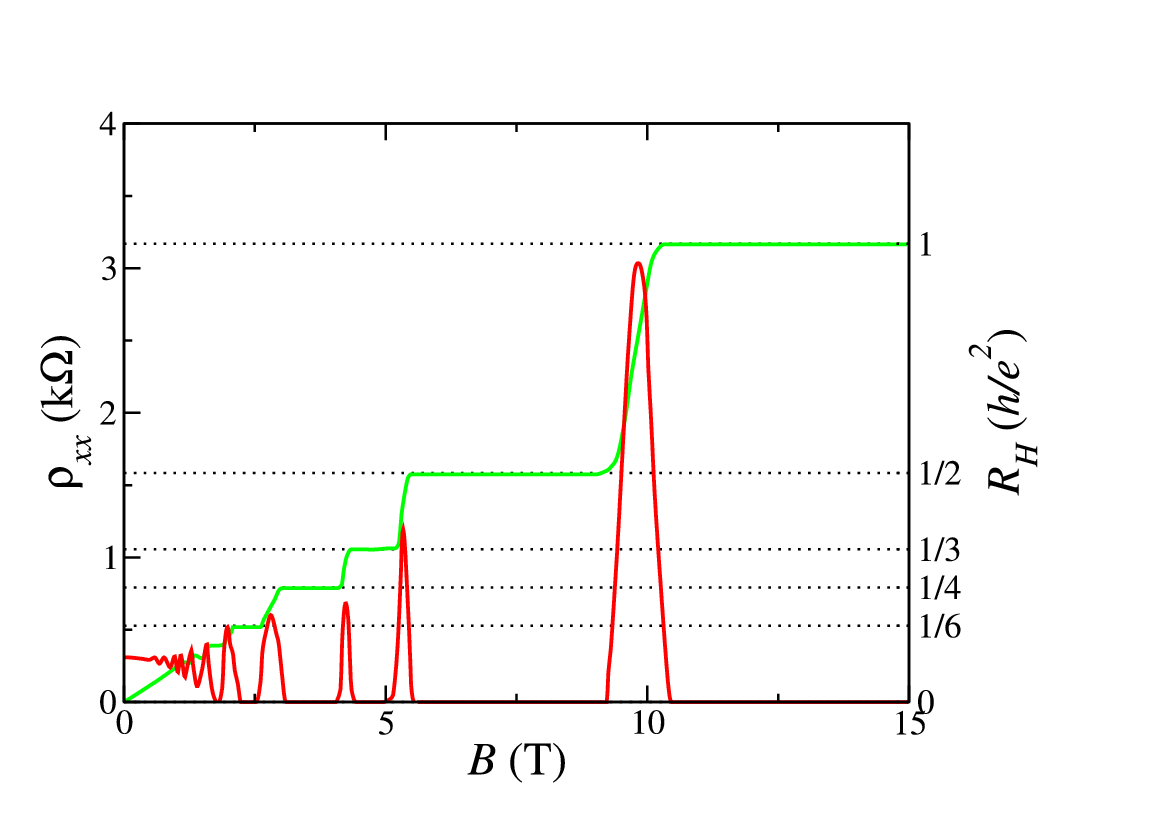
\includegraphics[width=\textwidth]{figures/quantum_hall_effect.png}
\end{center}

It can be seen that $\rho_{xy}$ develops perfectly flat plateaus exactly when $\rho_{xy} = h / e^2 \nu$ where $\nu$ is an integer (this is why we refer to this phenomena as the \term{integer quantum hall effect}; this contrasts the \term{fractional quantum hall effect} where $\nu$ is permitted to be any fraction). In fact $\nu$ is called the integer Landau level filling factor corresponding to the number of completely filled Landau levels. \\

The states at the center of each Landau level are delocalized and can contribute to transport. States in the tails of each Landau level are localized and can not contribute to transport. When considering $k_B T \ll \hbar c$, the temperature of the system can be treated as effectively zero. In these cases, the Fermi-Dirac distribution $f\br{\vep}$
\[ f\br{\vep} = \f{1}{e^{\br{\vep - \mu}/kT} + 1} \]
Tends towards the following step function,
\[ \lim_{T \to 0} f\br{\vep} = \begin{cases}
    1 & \vep < \mu \\
    0 & \vep > \mu
\end{cases} \]
At this temperature scale, the chemical potential is effectively the the Fermi energy $\vep\tsb{F}$. This makes sense; the typically energy $\mu$ to add/remove an electron would be the equivalent to the edge state fermions $\vep\tsb{F}$. As the magnetic field increases the Landau occupancy $N_{\phi}$ increases letting $\vep\tsb{F}$ tend to zero at higher and higher energies. For a fixed total number of particles $N$,
\[ \nu = \left\lfloor{\f{N}{N_{\phi}}}\right\rfloor \eq \label{eq:nu}\]
Gives the total number of \textit{completely} filled Landau levels while the Fermi energy $\vep\tsb{F}$ is simply the energy of the maximal Landau level that is at least partially occupied.
\[ \vep\tsb{F} = E_{\nu + 1} = \hbar \w_c \br{\nu + \f32} \eq \label{eq:fermi} \]
Therefore $\vep\tsb{F} = \mu$ becomes a function of $B$ for fixed $N$,
\[ \mu\br{B} = \hbar \f{e B}{mc} \br{\left\lfloor{\f{N{2 \pi \hbar c}}{{L_xL_y eB}}}\right\rfloor + \f12} \]
For fixed $N$ as $B \to \inf$, the floor function eventually reaches zero and the chemical potential tends as a straight line with slope $\f{\hbar e}{2mc}$. In order to plot this function consider setting $\hbar = c = e = m = 1$ and defining fixed $\ti n = 2 \pi N / (L_xL_y)$,
\[ \mu\br{B} = B \br{\left\lfloor{\f{\ti n}{B}}\right\rfloor + \f32} \]
\begin{center}
    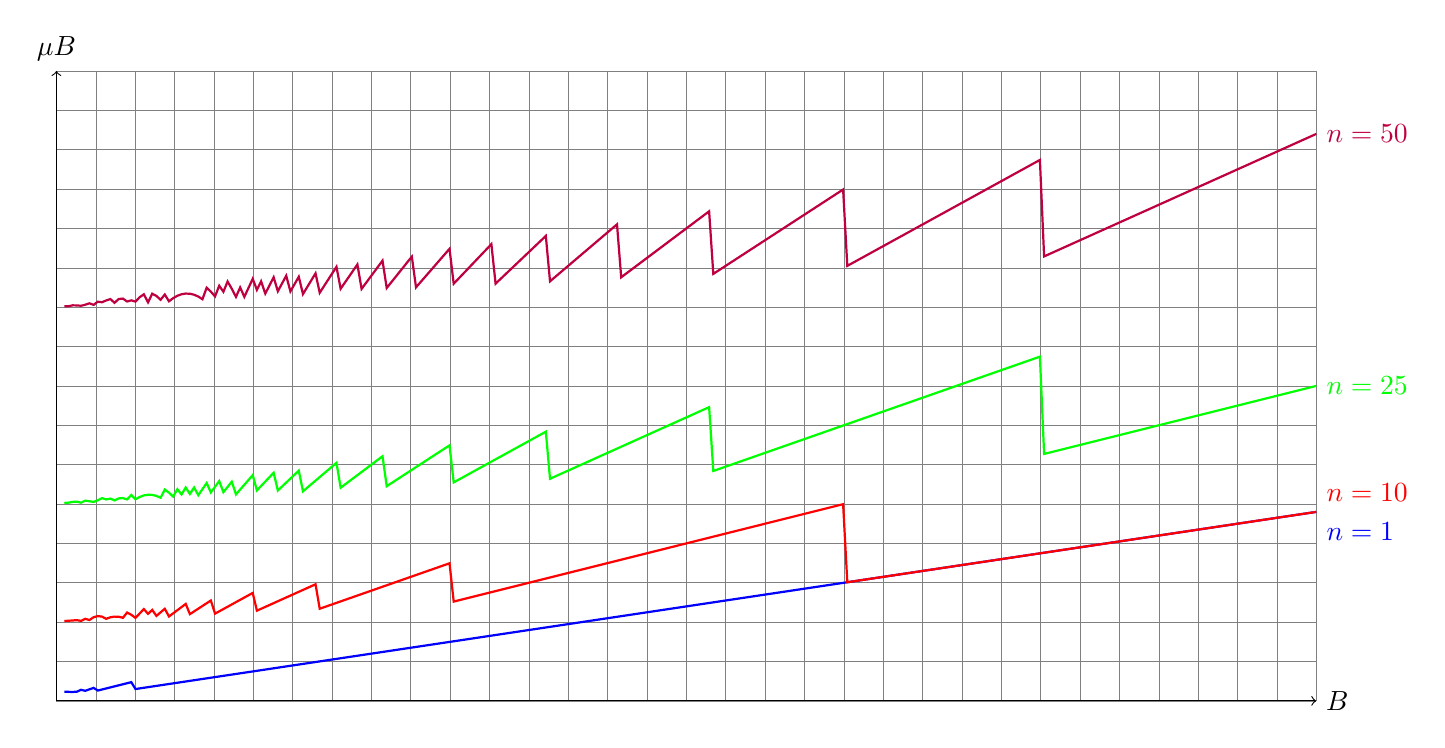
\begin{tikzpicture}
        \draw[step=.5cm,gray,very thin] (0,0) grid (16,8);
        % \draw[red, thick, domain=0:8, samples=300] plot (\x, {floor(\x)}) node[right] {$\lfloor x \rfloor$};
        % \draw[black,  thick, domain=0:8] plot(\x, \x) node[right] {$x$};
        % \draw[black, thick, domain=0:8] plot(\x, \x/2) node[right] {$x/2$};
        \draw[blue  , thick, domain=0.1:16, samples=300] plot(\x, {0.1*\x*(floor(( 1/\x)) + 3/2)})  node[below right] {$\ti n = 1$};
        \draw[red   , thick, domain=0.1:16, samples=300] plot(\x, {0.1*\x*(floor((10/\x)) + 3/2)})  node[above right] {$\ti n = 10$};
        \draw[green , thick, domain=0.1:16, samples=300] plot(\x, {0.1*\x*(floor((25/\x)) + 3/2)})  node[right] {$\ti n = 25$};
        \draw[purple, thick, domain=0.1:16, samples=300] plot(\x, {0.1*\x*(floor((50/\x)) + 3/2)})  node[right] {$\ti n = 50$};
        \draw [<->] (0,8) node[above]{$\mu\br{B}$} -- (0,0) -- (16,0) node[right]{$B$};
    \end{tikzpicture}
\end{center}

As the magnetic field increases, $N_{\phi} \propto B$ increases and $\vep\tsb{F}$ moves towards zero through the Landau levels. When $\vep\tsb{F}$ is in the mobility gap, the system behaves like an insulator while when it passes through the Landau level centers, it becomes metallic. This explains why nothing changes at the plateaus of $\rho_{xy}$ but doesn't explain why $\rho_{xy}$ is non-zero and quantized to precise values. This has to do with the existence of edge states. Consider a sample 2DEG that is finite in the $x$-direction admitting zero potential in regions between $\pm L_x / 2$ but approaches an infinite barrier at $V\br{\pm L_x / 2} = \inf$. Then the Schrödinger equation yields the familiar shifted harmonic oscillator with potential $V\br{x}$,
\[ \f{\hbar^2}{2m} \dder{\vp}{x} + \f{m\w_c^2}{2}\br{x + k_y \ell^2} \vp + V\br{x} \vp = E \vp \]
At $V = 0$, $\vp \sim e^{-\f{1}{2\ell^2}\br{x+k_y\ell^2}^2}$ varies on the scale of the magnetic length $\ell$. Suppose that $V\br{x}$ is very slowly varying on this scale. In this limit, we can solve the Schrödinger equation by simply replacing $V\br{x} \approx V\br{k_y \ell^2}$. The eigenvalues then become,
\[ E_{nk_y} = \hbar \w_c \br{n + \f12} + V\br{k_y \ell^2} \]
Thus when $\vep\tsb{F}$ is between the Landau levels in the bulk, there are still states at the Fermi energy of the edges of the system (called the edge states). Their number is equal to the number of filled Landau levels (edges are populated for each Landau level last). Moreover, near the intersection with $\vep\tsb{F}$ the dispersion is \textit{chiral},
\[ E_{n k_y} \simeq \vep\tsb{F}\pm\hbar v_n \br{k_y \pm k_{y,n}} \]
As we have seen before in \cref{eq:chrial_dispersion}, the existence of the chiral edge states implies the Hall effect,
\[ I_y = -e \int \f{\dif k}{2 \pi} v n\tsb{F}\br{\vep_k} \]
Since $\dif k = \dif \vep / \hbar v$,
\[ I_R = - \f{e}{2\pi \hbar}\int_{-\inf}^{\vep\tsb{FR}} \dif \vep n\tsb{F}\br{\vep} \]
\[ I_L = + \f{e}{2\pi \hbar}\int_{-\inf}^{\vep\tsb{FL}} \dif \vep n\tsb{F}\br{\vep} \]
Therefore,
\[ I_y = I_R + I_L = -\f{e}{h} \br{\vep\tsb{FR} - \vep\tsb{FL}} = -\f{e^2}{h}V_x \]
Such each filled Landau level contributes $\si_{yx} = - e^2 / h$ to the total Hall conductivity. Using the Landau level filling factor $\nu$,
\[ \si_{yx} = - \f{e^2}{h} \nu \]
Analogously,
\[ \si_{xy} = + \f{e^2}{h} \nu \]
As long as $\vep\tsb{F}$ is in the \textit{mobility gap} between Landau levels, $\si_{xy}$ stays pinned at this value since the number of edge states doesn't change and the bulk states don't contribute. Therefore,
\[ \si = \begin{pmatrix}
    0 & + \f{e^2}{h}\nu \\
    - \f{e^2}{h}\nu & 0 \\
\end{pmatrix} \]
The resistivity tensor is defined such that,
\[ \rho_{xx} = \f{\si_{xx}}{\si_{xx}^2 + \si_{xy}^2} = 0 \]
\[ \rho_{xy} = -\f{\si_{xy}}{\si_{xx}^2 +\si_{xy}^2} = - \f{1}{\si_{xy}} = - \f{h}{e^2} \nu \]
Amazingly, $\rho_{xx}$ and $\si_{xx}$ are zero simultaneously. Therefore a 2DEG in the quantum Hall regime behaves both as perfect insulator and a perfect conductor (in the appropriate directions).

\subsubsection{Conclusion}

The topological features of electronic structures we have considered thus far are genuine manifestations of quantum mechanics on macroscopic scales. For example, resistivity in the Quantum Hall effect,
\[ \rho_{xy} = \f{h}{e^2 \nu} \]
Has dependence on Planck's constant $h$ which indicates that it has no classical counterpart. This is in contrast with the Classical Hall effect,
\[ \rho_{xy} = \f{B}{nec} \]
which does not rely on quantum mechanics whatsoever. This concludes the first focus of this course and one of the major ideas in condensed matter physics: the effects of the electronic structure topology on macroscopic scales. \\

\section{Electron-electron Interactions}

Heretofore, we have consider materials where electrons are modeled as moving in a atomic lattice in \textit{isolation}. In essence, the electrons are treated as being non-interacting. This approximation was well-founded as many material properties can be seen as consequences of non-interacting electrons and in most cases, electron interactions are negligible. \\

However, in specific cases the electron interactions yield interesting physics. For example Landau Fermi liquid theory, magnetism and superconductivity all require a description of electronic interactions. \\

In particular, \term{ferro-magnetism} is the appearance of \textit{spontaneous} macroscopic magnetic momentum in certain materials at sufficiently low temperature $T$. For a material magnetic field $H$, the magnetization $M$ is
\[ M = \chi H \eq \label{eq:linear_susceptibility}\]
Where $\chi$ is the \term{magnetic susceptibility}.
\begin{itemize}
    \item $\chi > 0$ para-magnets
    \item $\chi < 0$ dia-magnets
\end{itemize}
Ferromagnets are distinct from both para and dia-magnets in that they possess magnetic fields $M \neq 0$ even in the absence of $H$. It is this feature we are referring to when we say that ferromagnets produce magnetic fields \textit{spontaneously}. \\

Unlike materials with completely filled shells (which have zero spin), materials that have incompletely filled d-shells (such as iron) have non-zero spin,
\[ \text{Fe} : 3 \text{d}^{6} 4\text{s}^2 \]
\term{Hund's rule} states that atomic orbitals are filled in such a way as to \textit{maximize} the total spin. Equivalently, any incompletely filled atomic orbital will always have non-zero total spin. If any incompletely filled shell has non-zero spin why are d-shells important? d-shells are important to magnetism because the electrons in higher orbital shells are spaced farther apart. This permits the electrons to have a stronger notion of localization for specific positions around atoms. \\

The combination of incompletely filled d-shells and Hund's rule implies that there is a non-zero atomic \term{magnetic moments $\ve \mu$},
\[ \ve \mu = g \mu_{B} \ve S \]
Where $\mu_B$ is the \term{Bohr magneton},
\[ \mu_{B} = \f{e\hbar}{2 mc} \]
And $g \approx 2$. Therefore,
\[ \mu \sim g \mu_B \sim \f{e\hbar}{mc} \]
The most obvious source interactions are magnetic dipole interactions
\[ U\tsb{dip} = \f{1}{r^3} \br{\ve \mu_1 \cdot \ve \mu_2 - 3 \br{\ve \mu_1 \cdot \hat r}\br{\ve \mu_2 \cdot \hat r}} \]
Recalling the Bohr radius $a_{0}$,
\[ a_{0} = \f{\hbar^2}{m c^2} \]
We can write $U\tsb{dip}$ in terms of a distance $r$,
\[ U\tsb{dip} \sim \f{\br{g\mu_B}^3}{r^3} = \br{\f{e\hbar}{mc}}^2 \f{1}{r^3} = \br{\f{e^2}{\hbar c}}^2 \f{e^2}{a_0} \br{\f{a_0}{r}}^3 \]
Where the coefficients are related to the dimensionless \term{Fine structure constant $\al$},
\[ \al = \f{e^2}{\hbar c} \simeq \f{1}{137} \]
Using this constant,
\[ U\tsb{sip} \sim \al^2 \f{e^2}{a_0} \br{\f{a_0}{r}}^3 \]
For typical atomic separations $r \sim a_0$, we have $U\tsb{dip} \sim \al^2 \f{e^2}{a_0} \sim \SI{e-4}{\eV}$ which corresponds to temperatures $T \sim U\tsb{dip}/k_B \sim \SI{1}{\K}$. This result is odd because we know that the critical temperature for iron is,
\[ \text{Fe} : T_c = \SI{1043}{\K} \]
Therefore dipole-dipole interactions can \textit{not} be the source of ferro-magnetism. \\

For ordinary electron-electron Coulomb interactions $e^2 / a_0$ is the typical Coulomb interaction energy between electrons on neighboring atoms.
\[ \f{e^2}{a_0} \sim \SI{1}{\eV} \qquad T \sim \SI{e4}{\K} \]
This is much closer to the critical temperature for iron, therefore we conclude that ordinary Coulumb interactions are responsible for ferro-magnetism. This result is surprising because the Coulumb potential does not know about magnetic fields; instead the effects of spin (in combination with $V\br{\ve r}$) will give rise to ferro-magnetism. \\

Consider $2$ electrons on two atomic orbitals $\vp_1\br{\ve r_1}$ and $\vp_2\br{\ve r_2}$ with the same energy. The Coulumb potential is,
\[ V\br{\ve r_1 - \ve r_2} = \f{e^2}{\abs{\ve r_1 - \ve r_2}} \]
In general the wave-function for the two electrons will depend on positions $\ve r_1, \ve r_2$ for the two electrons and spin values $\si_i \in \bc{\uu, \dd}$. This position and spin wave-functions are separable,
\[ \psi \br{\ve r_1 \si_1, \ve r_2 \si_2} = \psi\br{\ve r_1, \ve r_2} \chi \br{\si_1, \si_2} \]
Since the electrons are Fermions the wave-function must be antisymmetric with respect to the exchange of the two particles,
\[ \psi\br{\ve r_2 \si_2, \ve r_1 \si_1} = - \psi\br{\ve r_1 \si_1, \ve r_2\si_2} \]
Therefore we have two possibilities for the antisymmetry of $\psi$,
\begin{enumerate}
    \item $\psi\br{\ve r_1, \ve r_2}$ is antisymmetric:
    \[ \psi\br{\ve r_1, \ve r_2} = -\psi\br{\ve r_2, \ve r_1} \]
    \[ \chi\br{\si_1, \si_2} = +\chi\br{\si_2, \si_1} \]
    \item $\chi\br{\si_1, \si_2}$ is antisymmetric:
    \[ \psi\br{\ve r_1, \ve r_2} = +\psi\br{\ve r_2, \ve r_1} \]
    \[ \chi\br{\si_1, \si_2} = -\chi\br{\si_2, \si_1} \]
\end{enumerate}
Since the potential $V \br{\ve r_1 - \ve r_2}$ is independent of the spin, the total spin of two electrons is a conserved quantity. In using this observation, it is convenient to not label the individual spins $\si_1, \si_2$ (which are not conserved) but instead the total spin $S$ and its projection onto the $z$-axis $M$.
\[ \ket{\si_1, \si_2} \mapsto \ket{S, M} \]
If the total number states has to be conserved ($\ket{\si_1, \si_2} \in \s H^{2} \otimes \s H^{2} \implies \ket{S, M} \in \s H^{2} \otimes \s H^{2}$), then the four spin states,
\[ \ket{\uu, \uu} \quad\ket{\uu, \dd} \quad\ket{\dd, \uu} \quad\ket{\dd, \dd}  \]
Map to $4$ possible values for $S, M$. The $z$ component of the spin can take on any value from $1, 0, -1$ but the total magnitude of the spin must be either $0,1$.
\[ \ket{0, 0} \quad\ket{1, 1} \quad\ket{1, 0} \quad\ket{1, -1}  \]
Notice that these four states form and orthonormal basis for $\s H^2 \otimes \s H^{2}$. Explicitly these $\ket{S, M}$ states can be written as superpositions of the $\ket{\si_1, \si_2}$ states,
\begin{align*}
    \ket{1,1} & = \ket{\uu, \uu} \\
    \ket{1, -1} &= \ket{\dd, \dd} \\
    \ket{1,0} &= \f{1}{\sqrt{2}}\br{\ket{\uu, \dd} + \ket{\uu, \dd}} \\
    \ket{0,0} &= \f{1}{\sqrt{2}}\br{\ket{\uu, \dd} - \ket{\uu, \dd}}
\end{align*}
Importantly, each state $\ket{S, M}$ where the total spin $S$ is $S = 1$ is \textit{symmetric} with respect to the interchange of two electrons and the the spin $S = 0$ state is \textit{antisymmetric}. This anti-symmetry couples the spin states to the orbital components of the wave function. Since the spin $S=1$ states are symmetric, the wavefunction in position space with $S = 1$ must be anti-symmetric,
\[ \psi_{1M} \br{\ve r_1, \ve r_2} = \f{1}{\sqrt{2}}\br{\vp_1\br{\ve r_1} \vp_2\br{\ve r_2} - \vp_2\br{\ve r_1} \vp_1\br{\ve r_2}} \ket{1, M} \]
Analogously,
\[ \psi_{00} \br{\ve r_1, \ve r_2} = \f{1}{\sqrt{2}}\br{\vp_1\br{\ve r_1} \vp_2\br{\ve r_2} + \vp_2\br{\ve r_1} \vp_1\br{\ve r_2}} \ket{0, 0} \]
In order to determine the correction to the energy values due to the Coulumb interactions, use perturbation theory. Specifically, the $\psi_{1M}$ states are $3$-fold degenerate in position space but are distinct when spin states are included. Recalling that the corrections can be computed by calculating the matrix elements of the corrections $V$,
\begin{align*}
\bramidket{1,M}{V}{1,M}
&= \iint \dif^3 r_1 \dif^3 r_2 \f{1}{\sqrt{2}}\br{\vp^*_1\br{\ve r_1} \vp^*_2\br{\ve r_2} - \vp^*_2\br{\ve r_1} \vp^*_1\br{\ve r_2}} V\br{\ve r_1 - \ve r_2} \f{1}{\sqrt{2}}\br{\vp_1\br{\ve r_1} \vp_2\br{\ve r_2} - \vp_2\br{\ve r_1} \vp_1\br{\ve r_2}}\\
&= \f{1}{2}\iint \dif^3 r_1 \dif^3 r_2 V\br{\ve r_1 - \ve r_2} \bigg[\abs{\vp_1\br{\ve r_1}}^2 \abs{\vp_2\br{\ve r_2}}^2 + \abs{\vp_1\br{\ve r_2}}^2 \abs{\vp_2\br{\ve r_1}}^2  + \cdots\\
&\qquad \cdots - \vp_1^{*}\br{\ve r_1} \vp_2^{*}\br{\ve r_2}\vp_2\br{\ve r_1} \vp_1\br{\ve r_2} - \vp_2^{*}\br{\ve r_1} \vp_1^{*}\br{\ve r_2}\vp_1\br{\ve r_1} \vp_2\br{\ve r_2}\bigg]
\end{align*}
Recognize that since the potential only depends on the distance $\abs{\ve r_1, \ve r_2}$, our integral over $\ve r_1,\ve r_2$ counts each term twice. Therefore,
\begin{align*}
\bramidket{1,M}{V}{1,M}
&= \iint \dif^3 r_1 \dif^3 r_2 V\br{\ve r_1 - \ve r_2} \bigg[\abs{\vp_1\br{\ve r_1}}^2 \abs{\vp_2\br{\ve r_2}}^2 - \vp_1^{*}\br{\ve r_1} \vp_2^{*}\br{\ve r_2}\vp_2\br{\ve r_1} \vp_1\br{\ve r_2}\bigg]
\end{align*}
Similarly, we can calculate the matrix element for $\ket{0,0}$ (the elements $\bramidket{0,0}{V}{1, M}$ are zero),
\begin{align*}
\bramidket{0,0}{V}{0,0}
&= \iint \dif^3 r_1 \dif^3 r_2 V\br{\ve r_1 - \ve r_2} \bigg[\abs{\vp_1\br{\ve r_1}}^2 \abs{\vp_2\br{\ve r_2}}^2 + \vp_1^{*}\br{\ve r_1} \vp_2^{*}\br{\ve r_2}\vp_2\br{\ve r_1} \vp_1\br{\ve r_2}\bigg]
\end{align*}
Notice that $\bramidket{0,0}{V}{0,0}$ differs from $\bramidket{1,M}{V}{1,M}$ by the sign in the second set of terms. To facilitate discussions, let $\s C$ define the \term{Coulomb integral $\s C$},
\[ \s C = \iint \dif^3 r_1 \dif^3 r_2 V\br{\ve r_1 - \ve r_2} \bs{\abs{\vp_1\br{\ve r_1}}^2 \abs{\vp_2\br{\ve r_2}}^2} \]
Which is shared by both matrix elements and is a equivalent to a classical measurement of a Coulomb energy,
\[ \s C = \iint \dif^3 r_1 \dif^3 r_2 V\br{\ve r_1 - \ve r_2} \rho_1\br{\ve r_1}\rho_2\br{\ve r_2} \]
The differing integral is called the \term{exchange integral $\s J$},
\[ \s J = \iint \dif^3 r_1 \dif^3 r_2 V\br{\ve r_1 - \ve r_2} \bs{\vp_1^{*}\br{\ve r_1} \vp_2^{*}\br{\ve r_2}\vp_2\br{\ve r_1} \vp_1\br{\ve r_2}} \]
In conclusion,
\[ \bramidket{0,0}{V}{0,0} = \s C + \s J \qquad \bramidket{1,M}{V}{1,M} = \s C - \s J \]
The state with higher (or lower) energy correction will depend on the sign of $\s J$. If $\s J > 0$, this leads to alignment of the individual spins and to ferro-magnetism. Recalling $\psi_{1M} \br{\ve r_1, \ve r_2}$,
\[ \psi_{1M} \br{\ve r_1, \ve r_2} = \f{1}{\sqrt{2}}\br{\vp_1\br{\ve r_1} \vp_2\br{\ve r_2} - \vp_2\br{\ve r_1} \vp_1\br{\ve r_2}} \ket{1, M} \]
It can be seen that if we let $\ve r_1 = \ve r_2$ the antisymmetry forces,
\[ \psi_{1M} \br{\ve r_1, \ve r_1} = 0 \]
Therefore the probability of both electrons being found in the same place is zero and therefore the Coulomb interaction (which would normally tend to $\inf$ as $\ve r_1 \to \ve r_2$). Therefore the electrons tend toward their minimal energy state which corresponds to aligning their spins $S = 1$. An alternative way of seeing this is to consider $\s J$ in the case where $\ve r_1 = \ve r_2$, $\s J$ tends toward $\s C$ which is positive.\\

Let $\ve S = \ve S_1 + \ve S_2$ be the total spin operator for the two electrons. Therefore,
\[ \ve S^2 = \br{\ve S_1 + \ve S_2}^2 = \ve S_1^2 + \ve S_2^2 + 2 \ve S_1 \cdot \ve S_2 \]
Therefore the corrective energy is proportional to the product $\ve S_1 \cdot \ve S_2$,
\[ H = - \s J \ve S_1 \cdot \ve S_2 \]
Which is minimized for aligned spins $\ve S_1 \cdot \ve S_2 > 0$. This result can be generalized to any number of electron spins using the \term{Heisenberg model},
\[ H = -\f{1}{2} \s J \sum_{\ba{ij}} {\ve S_i \cdot \ve S_j} - g \mu_{B} \ve B \cdot \sum_{i} \ve S_i \eq \label{eq:Heisenberg_model}\]
Where $\ba{ij}$ denotes nearest neighbor terms, the factor of $1/2$ avoids double-counting the interactions, and $\s J$ forms a coupling constant proportional to,
\[ \s J \sim V \psi^2 \sim \f{e^2}{a_0} \]
And the $\mu_{B}$ terms is simply the ordinary magnetic moment coupling. It is important to note that the nearest-neighbor approximation permits one to assume that $\s J$ is a constant (depending only on the distance between nearest neighbors). The Heisenberg model \cref{eq:Heisenberg_model} is one of the simplest examples of a \term{quantum many-body problem} which are notoriously difficult to solve and are typically only approximated at best. The Heisenberg model cannot be solved exactly; one such approximation is called \term{mean-field theory}.

\subsection{Mean-field Theory of the Heisenberg Model}
% \label{sec:mft}
% Mean-field theory approximations of the Heisenberg model begin by re-writing the spins $\ve S_i$ as,
% \[ \ve S_i = \ve S_i - \ba{\ve S_i} + \ba{\ve S_i} \eq \label{eq:mft_approx}\]
% Therefore the spin product $\ve S_i \cdot \ve S_j$ includes many terms,
% \[ \ve S_i \cdot \ve S_j = \br{\ve S_i - \ba{\ve S_i} + \ba{\ve S_i}} \cdot \br{\ve S_j - \ba{\ve S_j} + \ba{\ve S_j}} \]
% \[ \ve S_i \cdot \ve S_j = \br{\ve S_i - \ba{\ve S_i}} \cdot \br{\ve S_j - \ba{\ve S_j}} + \ve S_i \cdot \ba{\ve S_j} + \ve S_j \cdot \ba{\ve S_i} - \ba{\ve S_i} \cdot \ba{\ve S_j} \eq \label{eq:mmf}\]
% The mean-field approximation assumes that the deviations of $\ve S_i$ from their mean $\ba{\ve S_i}$ is small,
% \[ \ve S_i = \ba{\ve S_i} + \s O\br{ \br{\ve S_i}^2} \]
% Therefore we can neglect the first term in \cref{eq:mmf} for being quadratic in the deviation,
% \[ \ve S_i \cdot \ve S_j \simeq \ve S_i \cdot \ba{\ve S_j} + \ve S_j \cdot \ba{\ve S_i} - \ba{\ve S_i} \cdot \ba{\ve S_j} \]
% Therefore \cref{eq:Heisenberg_model} becomes,
% \[ H = -\f{1}{2} \s J \sum_{\ba{ij}} \bs{\ve S_i \cdot \ba{\ve S_j} + \ve S_j \cdot \ba{\ve S_i} - \ba{\ve S_i} \cdot \ba{\ve S_j}} - g \mu_{B} \ve B \cdot \sum_{i} \ve S_i \eq \label{eq:shared_mft_approx}\]
% Notice that the first two terms $\br{\ve S_i \cdot \ba{\ve S_j}, \ve S_j \cdot \ba{\ve S_i}}$ are essentially $\ve S_i$ interacting with an effective magnetic field $\ve B\tsb{eff} \sim \ba{S_j}$. Furthermore, we will neglect the third term $\ba{\ve S_i} \cdot \ba{\ve S_j}$ for first analysis and include in back whenever its affects become relevant. Finally, we conclude that each spin shares the same expectation.
% \[ \ba{\ve S_i} = \ba{\ve S_j} = \ba{\ve S} \]
% Essentially $\ve S_i$ is independent of $i$. Our approximations have let us to the following Hamiltonian,
% \[ H = -\f{1}{2} \s J \sum_{\ba{ij}} \bs{\ve S_i \cdot \ba{\ve S} + \ve S_j \cdot \ba{\ve S}} - g \mu_{B} \ve B \cdot \sum_{i} \ve S_i \]
% Re-organizing the double counting,
% \[ H = -\s J \sum_{\ba{ij}} \ve S_i \cdot \ba{\ve S} - g \mu_{B} \ve B \cdot \sum_{i} \ve S_i \]
% Define the \term{z-coordination number} as the number of nearest neighbors for a given site $i$. We do this because the first summand is independent of $j$ which yields $z$ identical terms. Therefore,
% \[ H = -\s J z \ba{\ve S} \cdot \sum_{i} \ve S_i  - g \mu_{B} \ve B \cdot \sum_{i} \ve S_i \]
% We define the effective spin magnetic field as the \term{molecular field $\ve B_m$},
% \[ \ve B_m = J z \ba{\ve S} \eq \label{eq:Bm_Defined}\]
% While we redefine the true magnetic field to absorb the coefficients,
% \[ g \mu_B \ve B \mapsto \ve B \]
% Thus,
% \[ H = -\br{\ve B + \ve B_m} \cdot \sum_{i} \ve S_i \eq \label{eq:effect_molecular_magnetic_field} \]
% Recall that in \cref{eq:Heisenberg_model} we have the following terms,
% \[ H \sim - \f{1}{2}\s J \sum_{\ba{ij}} \ve S_i \cdot \ve S_j \]
% which possesses a symmetry with respect to an arbitrary rotations of all the spins. Therefore there is no preferred direction to the spin system in the absence of magnetic fields. However a particular direction is chosen subjected to the magnetic field $\ve B$. This is an example of \term{spontaneously broken symmetry} in which the arbitrary direction is chosen spontaneously. In regard to \cref{eq:effect_molecular_magnetic_field}, the energy is minimized when the spins are aligned and $\sum_i \ve S_i$ is maximized. If we choose the external magnetic field $\ve B$ to point in the $\hat z$ direction $\ve B = B \hat z$ we can conclude that the molecular magnetic field aligns itself in the same direction,
% \[ \ve B_m = B_m \hat z \]
% Therefore \cref{eq:effect_molecular_magnetic_field} simplifies,
% \[ H = -\br{B + B_m} \cdot \sum_{i} S_i^z \]
% At zero temperature, the spins will tend toward the minimal energy state when corresponds to the spins aligning with $S_i^z = \f12$. However at finite temperature,
% \[ \ba{S^z} = \f{\sum_{S^{z} = \pm 1/2} S^{z}e^{-\f{H_i}{k_B T}}}{\sum_{S^{z} = \pm 1/2} e^{-\f{H_i}{k_B T}}} \]
% Where $H_i$ is an individual Hamiltonian,
% \[ H_i = -\br{B + B_m} S_i^{z} \]
% Explicitly,
% \[ \ba{S^z} = \f{\sum_{S^{z} = \pm 1/2} S^{z}e^{\f{\br{B+B_m}S^{z}}{k_B T}}}{\sum_{S^{z} = \pm 1/2} e^{\f{\br{B+B_m}S^{z}}{k_B T}}} \]
% \[ \ba{S^z} = \f{1}{2}\f{e^{\f{\br{B+B_m}}{2k_B T}} - e^{-\f{\br{B+B_m}}{2k_B T}}}{e^{\f{\br{B+B_m}}{2k_B T}} + e^{-\f{\br{B+B_m}}{2k_B T}}} \]
% Recognize the hyperbolic trigonometric formulas,
% \[ \ba{S^z} = \f{1}{2}\f{\cosh \f{\br{B+B_m}}{2k_B T}}{\sinh \f{\br{B+B_m}}{2k_B T}} = \f12 \tanh \bs{\f{\br{B+B_m}}{2k_B T}} \]
% Recalling \cref{eq:Bm_Defined},
% \[ B_m = J z \ba{S^{z}} \]
% Which have the non-linear implicit equation for $B_m$ in terms of $B$.
% \[ B_m = \f{\s J z}{2} \tanh \bs{\f{\br{B+B_m}}{2k_B T}} \]
% Evidently, the molecular magnetic field will depend on the temperature $T$ and external magnetic field $B$. Alternatively, we can use this to find the expectation $\ba{S^{z}} \defined M$ as the \term{macroscopic magnetization per atom},
% \[ M = \f12 \tanh \bs{\f{B + \s J z M}{2 k_B T}} \eq \label{eq:main_magnetization_equation} \]

Begin with the Heisenberg model for many interacting spins $\bc{\ve S_i}$ ($i \in \bc{1,\ldots,N}$) subjected to an external magnetic field $\ve B$,
\[ H = -\f{1}{2} \s J \sum_{\ba{ij}} {\ve S_i \cdot \ve S_j} - g \mu_{B} \ve B \cdot \sum_{i} \ve S_i \eq \label{eq:heisenberg_model}\]
where $\ba{ij}$ indicates the sum is over nearest neighbor spins,
\[ \ba{ij} \defined \bc{\br{i,j} \in \bc{1,\ldots,N}^{2} \mid \text{$i$ and $j$ are nearest neighbors}} \]
the factor of $1/2$ avoids double-counting the interactions, the exchange integral $\s J$ is treated as a constant, $g$ is the spin g-factor of the electrons, and $\mu_B$ is the magnetic moment coupling constant.\\

Performing a mean-field approximation, we assert that the spins $\ve S_i$ variation (specifically $\ve S_i - \ba{\ve S_i}$) is small.
\[ \ve S_i = \ba{\ve S_i} + \s O \br{\ve S_i^2} \]
This permits us to write $\ve S_i \cdot \ve S_j$ in a form that exploits this mean-field theory approximation,
\begin{align*}
\ve S_i \cdot \ve S_j
&= \br{\ve S_i - \ba{\ve S_i} + \ba{\ve S_i}} \cdot \br{\ve S_j - \ba{\ve S_j} + \ba{\ve S_j}} \\
&= \br{\ve S_i - \ba{\ve S_i}} \cdot \br{\ve S_j - \ba{\ve S_j}} + \ve S_i \cdot \ba{\ve S_j} + \ve S_j \cdot \ba{\ve S_i} - \ba{\ve S_i} \cdot \ba{\ve S_j}
\end{align*}
Neglecting $\br{\ve S_i - \ba{\ve S_i}} \cdot \br{\ve S_j - \ba{\ve S_j}}$ as it is quadratic in the assumed small spin deviation, we obtain,
\[ H = -\f{1}{2} \s J \sum_{\ba{ij}} \bc{\ve S_i \cdot \ba{\ve S_j} + \ve S_j \cdot \ba{\ve S_i} - \ba{\ve S_i} \cdot \ba{\ve S_j}} - g \mu_{B} \ve B \cdot \sum_{i} \ve S_i \eq \label{eq:mmf_heisenberg_model_init}\]
Finally, make the approximation that each of the spins shared the same expectation,
\[ \ba{\ve S_i} = \ba{\ve S_j} = \ba{\ve S} \]
\[ H = -\f{1}{2} \s J \sum_{\ba{ij}} \bc{\ve S_i \cdot \ba{\ve S} + \ve S_j \cdot \ba{\ve S} - \ba{\ve S} \cdot \ba{\ve S}} - g \mu_{B} \ve B \cdot \sum_{i} \ve S_i \eq \label{eq:mmf_heisenberg_model_same_exp}\]
Noticing that each term in the summand of the $\s J$ term only depends on at most one index (either $i$ or $j$ or neither), we define the \term{$z$-coordination number} as the number of nearest neighbors for each atomic site $i$,
\[ z_i = \# \bc{\br{k, j} \in \bc{1,\ldots,N}^2 \mid \br{k,j} \in \ba{ij}} \]
and then assume that the lattice structure is such that $z_i = z$ is independent of $i$. Therefore \cref{eq:mmf_heisenberg_model_same_exp} becomes,
\[ H = -\f{1}{2} \s J z \ba{\ve S} \cdot \sum_{i} \bc{2\ve S_i - \ba{\ve S}} - g \mu_{B} \ve B \cdot \sum_{i} \ve S_i \eq \label{eq:mmf_heisenberg_model_z_coord} \]

At this stage it is notationally convenient to re-label a number of terms in this expression. The first is to renormalize the overall Hamiltonian by a constant,
\[ H \mapsto H - \f{1}{2}\s J zN \ba{\ve S}^2  \]
The second is to modify the units of $\ve B$ in order to eliminate the constants $g \mu_B$,
\[ \ve B \mapsto \f{1}{g \mu_{B}} \ve B \]
Therefore our Heisenberg model (\cref{eq:mmf_heisenberg_model_z_coord}) under these modifications becomes,
\[ H = - \br{\s J z \ba{\ve S} + \ve B} \cdot \sum_{i} \ve S_i \eq \label{eq:mmf_heisenberg_model} \]
Where $\ve B_m \defined \s J z \ba{\ve S}$ can be regarded as the \term{molecular magnetic field} generated by the spins of the material. Without loss of generality, fix the external magnetic field in the $\hat z$ direction ($\ve B = B \hat z$). Subject to this field, the energy of the system is minimized when $\ve B_m$ aligns in the same direction as $\ve B$ ($\ba{\ve S} \to \ba{S^z}\hat z$). Therefore we obtain,
\[ H = - \br{\s J z \ba{S^z} + B} \sum_{i} S_i^z \]
Recall that in \cref{eq:Heisenberg_model} we have the following terms,
\[ H \sim - \f{1}{2}\s J \sum_{\ba{ij}} \ve S_i \cdot \ve S_j \]
which possesses a symmetry with respect to an arbitrary rotations of all the spins. Therefore there is no preferred direction to the spin system in the absence of magnetic fields. However a particular direction is chosen subjected to the magnetic field $\ve B$. This is an example of \term{spontaneously broken symmetry} in which the arbitrary direction is chosen spontaneously. In regard to \cref{eq:mmf_heisenberg_model}, minimizing the energy of the system also forces $\sum_i S_i^z$ to become maximized (i.e. the spins all aligning in the same direction $S_i^z = \f12, \forall i$). However the minimal energy configuration is only accessible when the temperature $T$ is exactly zero. At finite temperature, each spin has a variety of accessible spin states $S_i^{z} \in \s S \defined \bc{-\f12, +\f12}$. Since $\ba{S^z}$ has be assumed to be the same for each site $i$, a finite temperature $T$ modifies $S_i^{z}$ such that $H_i \defined - \br{\s J z \ba{S^z} + B} S_i^z$ is increased (by decreasing $S_i^{z}$) in accordance with the increase $T$ in a manner independent of $i$. Therefore one can construct a partition function for the accessible spins states $\s S$ which will take on the same form for each $S_i^z$,
\[ Z \defined \sum_{S^z \in \s S} \exp\bs{-\f{H}{k_BT}} = \sum_{S^z \in \s S} \exp\bs{\f{\br{B_m + B} S^{z}}{k_BT}} \eq \label{eq:partition}\]
Therefore the spin expectation will be,
\[ \ba{S^z} = \f{1}{Z} \sum_{S^z \in \s S} S^z \exp\bs{\f{\br{B_m + B} S^{z}}{k_BT}} \eq \label{eq:partition_expectation}\]
Explicitly,
\[ Z = \exp\bs{-\f{{B_m + B}}{2k_BT}} + \exp\bs{\f{{B_m + B}}{2k_BT}} = 2 \cosh\bs{\f{{B_m + B}}{2k_BT}} \]
\[ \ba{S^z} = \f{1}{Z} \bc{\f12 \exp\bs{\f{{B_m + B}}{2k_BT}} -\f12 \exp\bs{-\f{{B_m + B}}{2k_BT}}} = \f{1}{2Z} 2 \sinh\bs{\f{{B_m + B}}{2k_BT}} = \f12 \tanh\bs{\f{B_m + B}{2k_B T}} \]
Therefore the macroscopic magnetization per atom $M \defined \ba{S^{z}}$ must satisfy the following implicit formula,
\[ M = \f12 \tanh\bs{\f{\s J z M + B}{2k_B T}} \eq \label{eq:main_magnetization_equation} \]
In order to study \textit{spontaneous} magnetization, we set the external field $\ve B$. In the absence of an external magnetic field $\ve B = \ve 0$, we assume that there material magnetizes spontaneously (and spontaneously breaks rotation symmetry) if and only if \cref{eq:main_magnetization_equation} has a solution for the given temperature $T$.
\[ M = \f12 \tanh\bs{\f{\s J z M}{2k_B T}} \eq \label{eq:magnetization_M}\]
For visualization, consider a re-scaling of the temperature parameter $\s T \defined \f{2 k_B T}{\s J z}$ such that \cref{eq:magnetization_M} becomes,
\[ M = \f12 \tanh\bs{\f{M}{\s T}} \eq \label{eq:1_solution_point} \]
When plotted, the solutions (or absence of solutions becomes clearer). Since $\tanh \br{0} = 0$, there is always a solution of $M = 0$ at all temperatures. If the slope of the RHS of \cref{eq:1_solution_point} is ever greater than a slope of $1$, there are two non-trivial solutions $M = \pm M_0$. This transition between no magnetization and magnetization is a phase transition and occurs at a \term{critical temperature} of $\s T_c = 1$ which corresponds to,
\[ 1 = \der{}{M} \bc{\f{1}{2}\tanh\bs{\f{M}{\s T}}} \bigg|_{M = 0} = {\f{1}{2\s T}\text{sech}^2\bs{\f{M}{\s T}}} \bigg|_{M = 0} = \f{1}{2 \s T} \implies \s T_c = \f12 \implies T_c = \f{\s J z}{4 k_B}\]
\begin{center}
    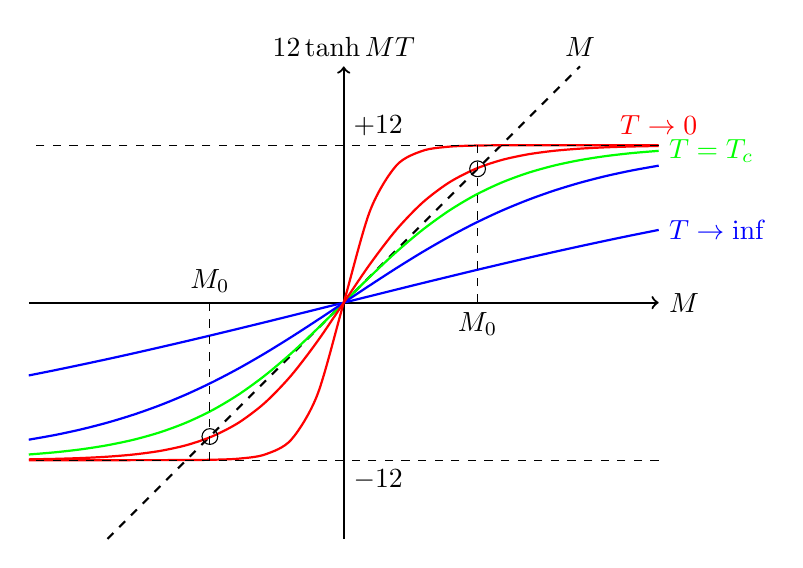
\begin{tikzpicture}
        \draw[thick, ->] (-4, 0) -- (+4, 0) node[right]{$M$};
        \draw[thick, ->] (0, -3) -- (0, +3) node[above]{$\f12\tanh\f{M}{\s T}$};
        \draw[thick,domain=-3:3,smooth,variable=\M,black,dashed] plot ({\M},{\M}) node[above]{$M$};
        \draw[thick,domain=-4:4,smooth,variable=\M,green] plot ({\M},{4*0.5*tanh(1/2 * \M)}) node[right]{$\s T = \s T_c$};
        \draw[thick,domain=-4:4,smooth,variable=\M,blue ] plot ({\M},{4*0.5*tanh(1/3 * \M)}) node[right]{};
        \draw[thick,domain=-4:4,smooth,variable=\M,blue ] plot ({\M},{4*0.5*tanh(1/8 * \M)}) node[right]{$\s T \to \inf$};
        \draw[thick,domain=-4:4,smooth,variable=\M,red  ] plot ({\M},{4*0.5*tanh(3/4 * \M)}) node[right]{};
        \draw[thick,domain=-4:4,smooth,variable=\M,red  ] plot ({\M},{4*0.5*tanh(2   * \M)}) node[above]{$\s T \to 0$};
        \draw[dashed] (+1.7,0) node[below]{$M_0$} -- (+1.7,+2);
        \draw[] (1.7+0.1,1.7) arc (0:360:0.1);
        \draw[dashed] (-1.7,0) node[above]{$M_0$} -- (-1.7,-2);
        \draw[] (-1.7+0.1,-1.7) arc (0:360:0.1);
        \draw[dashed] (+4, +2) -- node[above right]{$+\f12$} (-4, +2);
        \draw[dashed] (+4, -2) -- node[below right]{$-\f12$} (-4, -2);
    \end{tikzpicture}
\end{center}

The critical temperature distinguishes two different phases of the material,
\begin{itemize}
    \item $T < T_c$ ferro-magnetism
    \item $T < T_c$ no ferro-magnetism
\end{itemize}
For iron we have $\s J \sim \SI{1}{\eV}$ and $T \sim \SI{e4}{\K}$. This is an example of a \term{phase transition}.
\begin{center}
    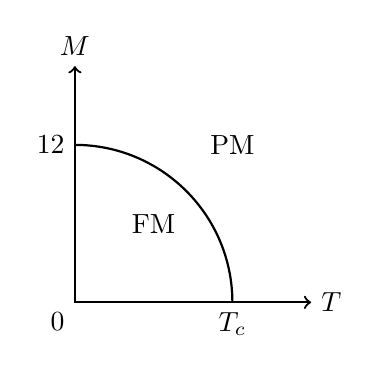
\begin{tikzpicture}
        \draw[thick,<->] (3, 0) node[right]{$T$} -- (0,0) node[below left]{$0$} -- (0, 3) node[above]{$M$};
        \draw[thick] (0,2) arc (90:0:2);
        \draw[thick] (2, 0) node[below]{$T_c$};
        \draw[thick] (0, 2) node[left]{$\f12$};
        \draw[thick] (1,1) node[]{FM};
        \draw[thick] (2,2) node[]{PM};
    \end{tikzpicture}
\end{center}
We refer to $M$ as the \term{M-order parameter} which allows us to formally distinguish between ferro-magnets and para-magnets. We have $M \neq 0$ in the FM phase but $M=0$ in the PM phase. \\

Depending on the nature of the phase transition boundary, we can have two types of phase translations: \term{first order phase translations} which are discontinuous or \term{second order phase transitions} which are continuous (as is the case for this phase transition).

\begin{center}
    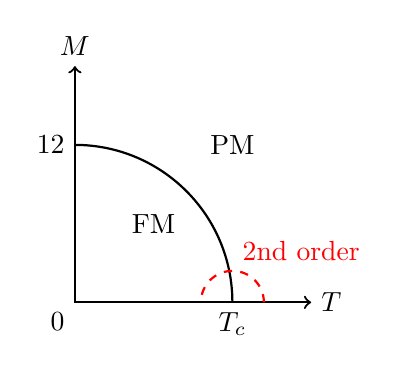
\begin{tikzpicture}
        \draw[thick,<->] (3, 0) node[right]{$T$} -- (0,0) node[below left]{$0$} -- (0, 3) node[above]{$M$};
        \draw[thick] (0,2) arc (90:0:2);
        \draw[thick,red,dashed] (2+0.4,0) arc (0:180:0.4) node[above right,midway]{2nd order};
        \draw[thick] (2, 0) node[below]{$T_c$};
        \draw[thick] (0, 2) node[left]{$\f12$};
        \draw[thick] (1,1) node[]{FM};
        \draw[thick] (2,2) node[]{PM};
    \end{tikzpicture}
    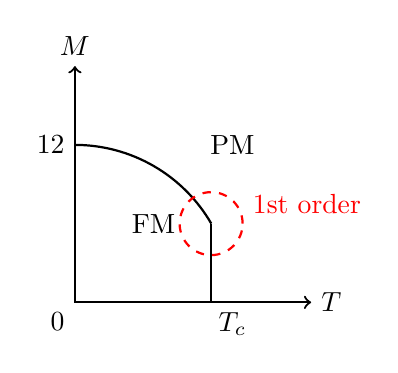
\begin{tikzpicture}
        \draw[thick,<->] (3, 0) node[right]{$T$} -- (0,0) node[below left]{$0$} -- (0, 3) node[above]{$M$};
        \draw[thick] (0,2) arc (90:30:2);
        \draw[thick,red,dashed] (1.73+0.4,1) arc (0:360:0.4) node[above right]{1st order};
        \draw[thick] (1.73, 0) -- (1.73, 1);
        \draw[thick] (2, 0) node[below]{$T_c$};
        \draw[thick] (0, 2) node[left]{$\f12$};
        \draw[thick] (1,1) node[]{FM};
        \draw[thick] (2,2) node[]{PM};
    \end{tikzpicture}
\end{center}

Given that $M$ vanishes continuously as $T$ increases, we can Taylor series \cref{eq:magnetization_M} near $T = T_c$,
\[ M = \f12 \bs{\f{\s J z M}{2 k_B T} - \f13 \br{\f{\s J z M}{2 k_B T}}^3} \]
Recalling the form of $T_c$ we cancel $M$ and obtain a quadratic equation for $M$,
\[ 1 = \f{T_c}{T} - \f13 \br{\f{T_c}{T}}^3 M^2 \]
Therefore $M^2$ as a function of temperature (at least near $T \simeq T_c$) can be written as,
\[ M^2 = \f{3}{4} \br{\f{T}{T_c}}^3 \br{\f{T_c}{T} - 1} \]
\[ M = \pm \f{1}{2} \f{T}{T_c} \sqrt{3\br{1 - \f{T}{T_c}}} \]
Since $T \simeq T_c$ we can neglect the prefactor,
\[ M\br{T} = \pm \f{1}{2}\sqrt{3\br{1 - \f{T}{T_c}}} \]
Therefore near the critical temperature we have,
\[ M\br{T} \sim \sqrt{T_c - T} \]
Defining the \term{reduced temperature} $t$,
\[ t = \f{T- T_c}{T_c} \]
We have that $M\br{t}$ behaves as follows,
\[ M\br{t} \simeq \br{- t}^{\be} \eq \label{eq:critical_exponent_onehalf}\]
Where $\be = \f12$ is called the \term{critical exponent}. In general (and as in this example), the critical exponent is typically some number $\be \in \R$ that is independent of the microscopic details of the material (like $\s J$ for example). Since $\be$ entirely determines the nature of the phase transition, we consider $\be$ to be a universal behaviour and is of particular interest. This universality is analogous to the Quantum Hall effect in which the conductivity is only dependent on universal constants. \\

The \term{magnetic susceptibility $\chi$} (first introduced in \cref{eq:linear_susceptibility}) in general is defined as,
\[ \chi = \der{M}{B} \]
For the mean-field theory approximations of the Heisenberg model we have obtained,
\[ M = \f12 \tanh \br{\f{B + \s J z M}{2 k_B T}} \]
Which for $T > T_c$ if $B \approx 0$ is small, the magnetization is also small $M \approx 0$. Expanding in Taylor series once again,
\[ M = \f{1}{2} \f{B + \s J z M}{2 k_B T} \]
Solving for $M$ as a response function of $B$,
\[ M = \f{B}{4 k_B T} + M \f{\s J z}{4 k_B T} \]
\[ M\br{1- \f{\s J z}{4 k_B T}} = \f{B}{4 k_B T} \]
\[ M\br{1- \f{T_c}{T}} = \f{B}{4 k_B T} \]
\[ M = \br{1- \f{T_c}{T}}^{-1}\f{B}{4 k_B T} \]
Therefore the magnetic susceptibility is $\chi$,
\[ \chi = \f{M}{B} = \f{1}{4 k_B \br{T- T_c}} \]
This is known as the \term{Cure-Weiss law}. Notice that this is consistent with our classification of paramagnets (which have $\chi > 0$ and $T > T_c$). Notice that $\chi$ diverges when $T \to T_c$; this is an alternative form of critical behaviour with critical exponent $\ga = -1$,
\[ \chi \sim \br{t}^{\ga} \eq \label{eq:sus_crit_exp} \]
The divergence of susceptibility is an example of non-analytic behaviour in a real physical system. The physical meaning of $\chi$ tells you how strongly $M$ responds to $B$.
\begin{center}
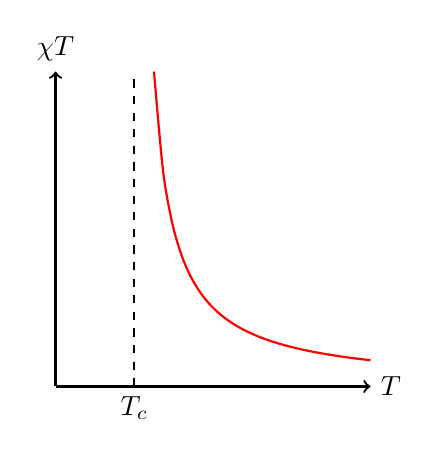
\begin{tikzpicture}
    \pgfmathsetmacro{\axissize}{4};
    \pgfmathsetmacro{\plotsize}{3};
    \pgfmathsetmacro{\tc}{1};
    \draw[thick, ->] (0,0) -- (+\axissize,0) node[right]{$T$};
    \draw[thick, ->] (0, 0) -- (0,+\axissize) node[above]{$\chi\br{T}$};
    \draw[thick, scale=1.0,domain=0.25:\plotsize,smooth,variable=\T,red] plot ({\T+\tc},{1/(\T)});
    \draw[thick, dashed] (\tc, 0) node[below]{$T_c$} -- (\tc, \axissize);
\end{tikzpicture}
\end{center}
The susceptibility $\chi$ diverges at $T = T_c$ because when $T < T_c$ we have spontaneous magnetization ($M \neq 0$) even in the absence of $B = 0$.

\subsection{Arbitrary Spin Systems}

In \label{sec:mft}, we performed mean-field theory analysis on the Heisenberg model \cref{eq:heisenberg_model} where the accessible spin states for the electrons formed the smallest possible set $\s S = \bc{-\f12, +\f12}$ which were the possible $S^{z}$ values for a particle with intrinsic spin of $S = \f12$. Instead we consider a particle with intrinsic spin $S \in \bc{0, \f12, 1, \f32, 2, \ldots}$ such that,
\[ \s S = \bc{-S, -S + 1, \ldots, S - 1, S} \]
Of course we can immediately disregard the trivial case of $S = 0$ whereby there is no magnetization because the Heisenberg model is trivially zero. \\

Returning to the partition function \cref{eq:partition},
\[ Z = \sum_{S^z \in \s S} \exp\bs{-\f{H}{k_BT}} = \sum_{S^z \in \s S} \exp\bs{\f{\br{B_m + B} S^{z}}{k_BT}} \]
Explicitly if we let $k$ be an index associated with the sum over spins defined such that $k = \s S + S$,
\[ k \in \bc{0, 1, \ldots, 2S - 1, 2S} \]
Also let $\eta \defined \exp\bs{\f{\br{B_m + B}}{k_BT}}$,
\begin{align*}
Z
&= \sum_{S^z \in \s S} \exp\bs{\f{\br{B_m + B} S^{z}}{k_BT}} \\
&= \sum_{k = 0}^{2S} \eta^{\br{k - S}} \\
&= \sum_{k = 0}^{2S} \eta^{k} \eta^{-S} \\
&= \f{1}{\eta^{S}}\sum_{k = 0}^{2S} \eta^{k} \\
&= \f{1}{\eta^{S}}\br{\sum_{k = 0}^{\inf} \eta^{k} - \sum_{k = 2S}^{\inf} \eta^{k}} \\
&= \f{1}{\eta^{S}}\br{\sum_{k = 0}^{\inf} \eta^{k} - \eta^{2S}\sum_{k = 2S+1}^{\inf} \eta^{k - 2S}} \\
&= \f{1}{\eta^{S}}\br{\sum_{k = 0}^{\inf} \eta^{k} - \eta^{2S+1}\sum_{k = 0}^{\inf} \eta^{k}} \\
&= \f{1- \eta^{2S+1}}{\eta^{S}}\sum_{k = 0}^{\inf} \eta^{k}
\end{align*}
Ignoring the fact that $\abs{\eta} = \abs{\exp\bs{\f{\br{B_m + B}}{k_BT}}} \not < 1$, we can make use of the geometric series (confident that the expression is convergent because the original sum was finite),
\[ Z = \f{1- \eta^{2S+1}}{\eta^{S}\br{1 - \eta}} \eq \label{eq:derivative} \]
Additionally we may make use of an arithmetic series to derive the expectation value $\ba{S^{z}}$ (analogous to \cref{eq:partition_expectation}),
\[ \ba{S^z} = \f{1}{Z} \sum_{S^z \in \s S} S^z \exp\bs{\f{\br{B_m + B} S^{z}}{k_BT}} = \f{1}{Z} \sum_{k = 0}^{2S} \br{k - S} \eta^{k - S}\]
\begin{align*}
    \ba{S^z}
    &= \f{1}{Z} \sum_{k = 0}^{2S} \br{k - S} \eta^{k - S} \\
    &= \f{1}{Z\eta^{S}} \bc{\sum_{k = 0}^{2S} k \eta^{k} - S\sum_{k = 0}^{2S} \eta^{k}} \\
    &= \f{1}{Z\eta^{S}} \bc{\sum_{k = 0}^{2S} k \eta^{k} - S \eta^{S} Z} \\
    &= \f{1}{Z\eta^{S}} \bc{\eta\sum_{k = 0}^{2S} k \eta^{k-1} - S\eta^{S}Z} \\
    &= \f{1}{Z\eta^{S}} \bc{\eta\sum_{k = 0}^{2S} \der{\eta^{k}}{\eta} - S\eta^{S}Z} \\
    &= \f{1}{Z\eta^{S}} \bc{\eta\der{}{\eta}\sum_{k = 0}^{2S} \eta^{k} - S\eta^{S}Z} \\
    &= \f{1}{Z\eta^{S}} \bc{\eta\der{}{\eta}\br{\eta^{S}Z} - S\eta^{S}Z}
\end{align*}
Taking the derivative of \cref{eq:derivative},
\begin{align*}
\der{}{\eta}\br{\eta^{S}Z}
&= \der{}{\eta}\bc{\eta^{S}\f{1- \eta^{2S+1}}{\eta^{S}\br{1 - \eta}}} \\
&= \der{}{\eta}\bc{\br{1- \eta^{2S+1}}\br{1 - \eta}^{-1}} \\
&= - \br{2S+1}\eta^{2S}\br{1 - \eta}^{-1} + \br{1- \eta^{2S+1}}\br{1 - \eta}^{-2} \\
\end{align*}
Therefore,
\[ \eta\der{}{\eta}\br{\eta^{S}Z} - S\eta^{S}Z = - \br{2S+1}\eta^{2S+1}\br{1 - \eta}^{-1} + \eta\br{1- \eta^{2S+1}}\br{1 - \eta}^{-2} - S\br{1- \eta^{2S+1}}\br{1 - \eta}^{-1}  \]
\[ \ba{S^z} = \f{1}{Z\eta^{S}}\bc{- \br{2S+1}\eta^{2S+1}\br{1 - \eta}^{-1} + \eta\br{1- \eta^{2S+1}}\br{1 - \eta}^{-2} - S\br{1- \eta^{2S+1}}\br{1 - \eta}^{-1}}  \]
\[ \ba{S^z} = \f{1}{Z\eta^{S} \br{1 - \eta}^2}\bc{- \br{2S+1}\eta^{2S+1}\br{1 - \eta} + \eta\br{1- \eta^{2S+1}} - S\br{1- \eta^{2S+1}}\br{1 - \eta}}  \]
\[ \ba{S^z} = \f{1}{Z\eta^{S} \br{1 - \eta}^2}\bc{2S\eta^{2S+1}\br{\eta-1} - \eta^{2S+1}\br{1 - \eta} + \eta\br{1- \eta^{2S+1}} + S\br{1- \eta^{2S+1}}\br{\eta - 1}}  \]
\[ \ba{S^z} = \f{1}{Z\eta^{S} \br{1 - \eta}^2}\bc{- \br{\eta^{2S+1} - \eta^{2S+2}} - \br{\eta^{2S+2} - \eta} + S\br{1 + \eta^{2S+1}}\br{\eta - 1}}  \]
% Therefore
% \[ \ba{S^z} = \f{1}{Z\eta^{S}} \bc{\f{\eta}{1 - \eta} \br{Z-S\eta^{-S-1} - S\eta^{S} - \eta^{S}}  - SZ} \]
% \[ \ba{S^z} = \f{1}{Z\eta^{S}} \bc{\f{\br{2 S \br{\eta-1} - \eta \br{\eta^{2S} - 1}}}{\eta^{S}\br{1 - \eta}^2}} \]
% \[ \ba{S^z} = \f{\br{1 - \eta}}{1- \eta^{2S+1}}\bc{\f{\br{2 S \br{\eta-1} - \eta \br{\eta^{2S} - 1}}}{\eta^{S}\br{1 - \eta}^2}} \]
% \[ \ba{S^z} = \f{2 S \br{\eta-1} - \eta \br{\eta^{2S} - 1}}{\eta^{S}\br{1- \eta^{2S+1}}\br{1 - \eta}} \]
% \[ \ba{S^z} = \f{2 S \eta - 2S - \eta^{2S+1} + \eta}{\eta^{S}\br{1- \eta^{2S+1}}\br{1 - \eta}} \]
% By choosing $x = \f{\br{B_m + B}}{k_BT}$ we have $\eta = e^{x}$. Moreover,
% \[ \eta^{S} + \eta^{-S} = e^{Sx} + e^{-Sx} = 2 \cosh \br{Sx} \]
% \[ \eta^{S} - \eta^{-S} = e^{Sx} - e^{-Sx} = 2 \sinh \br{Sx} \]
% \[ Z = \f{\eta^{S} - \eta^{-S}}{\eta - 1} = 2 \f{\sinh \br{Sx}}{e^{x} - 1} \]
% ---
% \[ \ba{S^z} = \f{1}{Z\eta^{S}} \bc{\f{S\br{\eta-1}\br{\eta^{2S+1} + 1}}{\br{1 - \eta}^2} - \f{\eta\br{\eta^{2S} - 1}}{\br{1 - \eta}^2}} \]
\[ \ba{S^z} = \f{1}{Z\eta^{S}} \f{S\br{\eta-1}\br{\eta^{2S+1} + 1} - \eta\br{\eta^{2S} - 1}}{\br{1 - \eta}^2} \]
\[ \ba{S^z} = \f{1}{Z\eta^{S}} \f{S\br{\eta^{2S+2} + \eta - \eta^{2S+1} - 1} + \br{\eta - \eta^{2S+1}}}{\br{1 - \eta}^2} \]
\[ \ba{S^z} = \f{S\br{\eta^{2S+2} + \eta - \eta^{2S+1} - 1} + \br{\eta - \eta^{2S+1}}}{\br{\eta^{2S+1} - 1}\br{\eta - 1}} \]
\[ \ba{S^z} = \f{S\br{\eta^{2S+2} + \eta - \eta^{2S+1} - 1} + \f{1}{2}\br{\eta^{2S+2} + \eta - \eta^{2S+1} - 1 - \eta^{2S+2} + \eta - \eta^{2S+1} + 1}}{\br{\eta^{2S+1} - 1}\br{\eta - 1}} \]
\[ \ba{S^z} = \f{\f{2S+1}{2}\br{\eta^{2S+2} + \eta - \eta^{2S+1} - 1} - \f{1}{2}\br{\eta^{2S+2} - \eta + \eta^{2S+1} - 1}}{\br{\eta^{2S+1} - 1}\br{\eta - 1}} \]
\[ \ba{S^z} = \f{\f{2S+1}{2}\br{\eta^{2S+1} + 1}\br{\eta - 1} - \f{1}{2}\br{\eta^{2S+1} - 1}\br{\eta + 1}}{\br{\eta^{2S+1} - 1}\br{\eta - 1}} \]
\[ \ba{S^z} = \f{2S+1}{2} \f{\br{\eta^{2S+1} + 1}\br{\eta - 1}}{\br{\eta^{2S+1} - 1}\br{\eta - 1}} - \f{1}{2} \f{\br{\eta^{2S+1} - 1}\br{\eta + 1}}{\br{\eta^{2S+1} - 1}\br{\eta - 1}} \]
\[ \ba{S^z} = \f{2S+1}{2} \f{\eta^{2S+1} + 1}{\eta^{2S+1} - 1} - \f{1}{2} \f{\eta + 1}{\eta - 1} \]
Defining $\chi$ such that $\eta = e^{\chi}$,
\[ \ba{S^z} = \f{2S+1}{2} \f{e^{\br{2S+1} \chi} + 1}{e^{\br{2S+1} \chi} - 1} - \f{1}{2} \f{e^{\chi} + 1}{e^{\chi} - 1} \]
\[ \ba{S^z} = \f{2S+1}{2} \coth \br{\f{2S+1}{2} \chi} - \f{1}{2} \coth \br{\f{1}{2} \chi} \]
\[ \ba{S^z} = S B_S\br{S \chi} \]
Where $B_S\br{x}$ is the Brillouin function,
\[ B_S \br{x} \defined \f{2S+1}{2S} \coth\br{\f{2S+1}{2S} x} - \f{1}{2S} \coth\br{\f{1}{2S} x} \]
Therefore analogously to \cref{eq:main_magnetization_equation} the magnetization $M \defined \ba{S^z}$ must satisfy the following equation,
\[ M = S B_S \br{\f{S\br{\s J z M + B}}{k_B T}} \]
In the absence of an external magnetic field we have (letting $\s T = k_B T / \s J z$),
\[ M = S B_S \br{\f{SM}{\s T}} \]
Since $\coth\br{x} = - \coth\br{-x}$ is odd symmetric, we have that,
\[ S B_S \br{\f{SM}{\s T}} = -S B_S \br{\f{S\br{-M}}{\s T}} \]
Therefore we can restrict our focus to potential solutions where $M \geq 0$ being confident that a negative $M$ solution exists as well. Next,
\[ S B_S \br{\f{SM}{\s T}} = \f{2S+1}{2} \coth \br{\f{2S+1}{2S} \f{M}{\s T}} - \f{1}{2} \coth \br{\f{1}{2S} \f{M}{\s T}} \]
For $M \geq 0$,
\[ S B_S \br{\f{SM}{\s T}} \geq \f{1}{2} \coth \br{\f{2S+1}{2S} \f{M}{\s T}} - \f{1}{2} \coth \br{\f{1}{2S} \f{M}{\s T}} \]
\[ S B_S \br{\f{SM}{\s T}} \geq \f{1}{2} \coth \br{\f{1}{2S} \f{M}{\s T}} - \f{1}{2} \coth \br{\f{1}{2S} \f{M}{\s T}} \]
\[ S B_S \br{\f{SM}{\s T}} \geq 0 \]
Finally,
\[ \der{}{\s M} \br{S B_S \br{\f{SM}{\s T}}} = \der{}{\s M}\bc{\f{2S+1}{2} \coth \br{\f{2S+1}{2S} \f{M}{\s T}} - \f{1}{2} \coth \br{\f{1}{2S} \f{M}{\s T}}} \]
\[ \der{}{\s M} \br{S B_S \br{\f{SM}{\s T}}} = -\f{2S+1}{2}\f{2S+1}{2S\s T}\text{csch}^2\br{\f{2S+1}{2S} \f{M}{\s T}} + \f{1}{2} \f{1}{2S\s T} \text{csch}^2 \br{\f{1}{2S} \f{M}{\s T}} \]
Since $\der{}{\s M} \br{S B_S \br{\f{SM}{\s T}}}$ as positive $M > 0$ solution exists if and only if $S B_S \br{\f{SM}{\s T}}$ has slope greater than $1$ at $M = 0$. This defines the critical temperature.
\[ \der{}{\s M} \br{S B_S \br{\f{SM}{\s T}}} \Bigg|_{M = 0} = \lim_{M \to 0^{+}} \bc{-\f{2S+1}{2}\f{2S+1}{2S\s T}\text{csch}^2\br{\f{2S+1}{2S} \f{M}{\s T}} + \f{1}{2} \f{1}{2S\s T} \text{csch}^2 \br{\f{1}{2S} \f{M}{\s T}} } \]
\[ \der{}{\s M} \br{S B_S \br{\f{SM}{\s T}}} \Bigg|_{M = 0} = \f{S \br{S+1}}{3 \s T} \]
\[ \s T_c = \f{S \br{S+1}}{3} \implies T_c = \f{\s J z}{k_B} \f{S \br{S+1}}{3} \]
Which for $S = 1/2$ we recover the usual $T_c = \f{\s J z}{4k_B}$.

\subsection{Mean-field Theory and Helmholtz Free Energy}
In the previous section (\cref{sec:mft}), we analyzed the mean-field theory approximation to the Heisenberg model $H$,
\[ H = -\f12 \s J \sum_{\ba{ij}} \ve S_i \cdot \ve S_j \]
Although very useful, the mean-field theory approximations fail an predicting all phenomena that are manifest in the Heisenberg model. Here we will make the same first approximations,
\[ \ve S_i = \ve S_i - \ba{\ve S_i} + \ba{\ve S_i} \eq \label{eq:nmft_approx}\]
And obtain the following,
\[ H = -\f{1}{2} \s J \sum_{\ba{ij}} \bs{\ve S_i \cdot \ba{\ve S_j} + \ve S_j \cdot \ba{\ve S_i} - \ba{\ve S_i} \cdot \ba{\ve S_j}} - g \mu_{B} \ve B \cdot \sum_{i} \ve S_i \eq \label{eq:shared_nmft_approx}\]
Letting $\ve B = B \hat z$ and assuming that the expectation of each $\ve S_i$ is magnetized as follows,
\[ \ba{\ve S_i} = M \hat z \qquad \forall i \]
To obtain the following Hamiltonian,
\[ H = \f{\s J z N}{2} M^2 - \br{\s J z M + B} \sum_{i} S_i^z \]
From this, we can define the \term{partition function $Z$} (as used in statistical mechanics) over the energy states,
\[ Z = \bs{\sum_{S^{z} = \pm 1/2} e^{- \f{\s J z M^2}{2k_BT} + \f{\s J z M S^{z}}{k_B T}}}^N \]
Such that the \term{Helmholtz free energy $F$} has the following form,
\[ F \defined E - TS = - k_B T \ln Z \]
Simplifying $Z$,
\[ Z = \bs{e^{- \f{\s J z M^2}{2k_BT} + \f{\s J z M}{2k_B T}} + e^{- \f{\s J z M^2}{2k_BT} - \f{\s J z M}{2k_B T}}}^N \]
\[ Z = e^{- \f{\s J z M^2 N}{2 k_B T}}\bs{e^{\f{\s J z M}{2k_BT}}+ e^{- \f{\s J Z M}{2k_B T}}}^N \]
\[ Z = e^{- \f{\s J z M^2 N}{2 k_B T}}\bs{2 \cosh\br{\f{\s J Z M}{2k_B T}}}^N \]
Therefore the free energy is,
\[F = \f{\s J z M^2 N}{2} - k_B T \ln\bs{2^N \cosh^N \br{\f{\s J z M}{2 k_B T}}} \]
\[F = \f{\s J z M^2 N}{2} - Nk_B T \ln\bs{2 \cosh \br{\f{\s J z M}{2 k_B T}}} \]
In order to find the equilibrium state of this system, we need to minimize the Helmholtz free energy with respect to $M$,
\[ \pder{F}{M} = \s J z M N - N k_B T \f{2 \f{\s J z}{2 k_B T} \sinh \br{\f{\s J z M}{2 k_B T}}}{2 \cosh \br{\f{\s J z M}{2 k_B T}}}\]
\[ \pder{F}{M} = \s J z M N - N k_B T \f{\s J z}{k_B T} \tanh \br{\f{\s J z M}{2 k_B T}} \]
Minimizing corresponds to setting $\pder{F}{M} = 0$. Doing so yields,
\[ M = \f12 \tanh \br{\f{\s J z M}{2 k_B T}} \]
Which is identical to \cref{eq:magnetization_M} as expected. This approach is simply an alternative method for deriving \cref{eq:magnetization_M}. Near $T = T_c$, we can expand $F\br{M}$ in Taylors series with respect to $M$. Defining $f$ to be $F / N$,
\[ f \defined \f{F}{N} = \f{\s J z M^2}{2} - k_B T \ln\bs{2 \cosh \br{\f{\s J z M}{2 k_B T}}} \]
As in turns out, we need to expand $f\br{M}$ to fourth order. Before doing so, notice that $f\br{M}$ is an even function in $M$ (which is equivalent to saying that $f\br{M} = f\br{-M}$). Therefore within the the first four orders, we have two non-zero terms.
\[ f\br{M} = \f{\s J z M^2}{2} - \f{k_B T}{2} \br{\f{\s J z M}{2 k_B T}}^2 + \f{k_B T}{12} \br{\f{\s J z M}{2 k_B T}}^4 + \s O \br{M^4} \]
For notational convenience, drop $\s O \br{M^4}$ and make use of natural units such that $k_B T \mapsto T$ where $T$ now has units of energy.
\[ f\br{M} = \f{\s J z M^2}{2} - \f{T}{2} \br{\f{\s J z M}{2 T}}^2 + \f{T}{12} \br{\f{\s J z M}{2 T}}^4 \]
Moreover, making use of the critical temperature $T_c$,
\[ f\br{M} = 2 T_c M^2 \br{1 - \f{T_c}{T}} + \f43 \f{T_c^4}{T^3} M^4 \]
Again since $T \approx T_c$ when $M \approx 0$ we can neglect prefactors,
\[ f\br{M} = 2 T_c \br{1 - \f{T_c}{T}} M^2 + \f43 T_c M^4 \]

\begin{center}
\begin{tikzpicture}
    \pgfmathsetmacro{\axissize}{4};
    \pgfmathsetmacro{\plotsize}{3};
    \draw[thick, ->] (-\axissize,0) -- (+\axissize,0) node[right]{$M$};
    \draw[thick, ->] (0,-\axissize) -- (0,+\axissize) node[above]{$f\br{M}$};
    \draw[thick, scale=1.0,domain=-1.5:1.5,smooth,variable=\T,red ] plot ({\T*4},{(\T)^2}) node[right]{$T > T_c$};
    \draw[thick, scale=1.0,domain=-1.5:1.5,smooth,variable=\T,blue ] plot ({\T*4},{(\T)^4 - (\T)^2}) node[right]{$T < T_c$};
    \draw[thick,blue,dashed] (2.9,0) -- (2.9, -0.4) node[below]{$M_0$};
    \draw[thick,blue,dashed] (-2.9,0) -- (-2.9, -0.4) node[below]{$-M_0$};
\end{tikzpicture}
\end{center}

As you can see when $T$ transitions from $T > T_c$ to $T < T_c$, two new free energy minima form at precisely $\pm M_0$.
\[ \pder{f}{M} = 0 \implies 0 = \pder{}{M}\br{2 T_c \br{1 - \f{T_c}{T}} M^2 + \f43 T_c M^4} = 4 T_c \br{1 - \f{T_c}{T}} M + \f{16}3 T_c M^3 \]
For $M \neq 0$ (which corresponds to a maximum of $f$ when $T < T_c$),
\[ 0 = 4 T_c \br{1 - \f{T_c}{T}} + \f{16}3 T_c M^2\]
\[ 4 T_c \br{\f{T_c}{T} - 1} = \f{16}3 T_c M^2\]
\[ M^2 = \f34\br{\f{T_c}{T} - 1}\]
\[ M = \pm M_0 \defined \pm \sqrt{\f34\br{\f{T_c}{T} - 1}}\]
The important scaling feature is that $M$ scales as,
\[ M \sim \br{\f{T_c - T}{T_c}}^{1/2} \]
For $M$ nearby $\pm M_0$; this is identical to the critical exponent of $\be = 1/2$ found earlier (\cref{eq:critical_exponent_onehalf}).

\subsection{Landau Theory}
Let us now return to out original Heisenberg model,
\[ H = - \f{\s J}{2}\sum_{\ba{ij}}\ve S_i \cdot \ve S_j \]
Notice that $H$ is invariant with respect to arbitrary rotation of all spins because $\ve S_i \cdot \ve S_j$ is preserved under rotations (note that this is a global symmetry of all spins simultaneously). If we define $\ve M$ to be a vector corresponding to all of the mean spins,
\[ \ve M \defined \ba{\ve S_i} \]
We induce the following free-energy density $f\br{\ve M}$ which depends on each of the independent spins. $f \br{\ve M}$ will have the same global symmetry of rotations. Therefore $f\br{\ve M}$ can only depend on $\ve M \cdot \ve M = \abs{\ve M}^2$ to various powers,
\[  f\br{\ve M} = a \ve M \cdot \ve M + \f{b}{2} \br{\ve M \cdot \ve M}^2 + \cdots \eq \label{eq:landau_theory_first}\]
Where $a, b = a\br{t}, b\br{t} \in \R$ are yet unknown coefficients that are parameterized by $t = \br{T-T_c}/T_c$. This remarkable result require no calculations, just symmetry arguments. When $\abs{t} \ll 1$, $T$ is very close to $T_c$. We expand out $a\br{t}$ and $b\br{t}$ in Taylor series of $t$,
\[ a\br{t} = a_0 + a_1 t + \cdots \qquad  b\br{t} = b_0 + b_1 t + \cdots \]
We can find $a_0, a_1$ and $b_0, b_1$ from the requirement that $\abs{\ve M} \neq 0$ when $t < 0$ ($T < T_c$) and $\abs{\ve M} = 0$ when $t > 0$ ($T > T_c$). Therefore for $f\br{\ve M}$,
\[ f\br{\ve M} = a \abs{\ve M}^2 + \f{b}{2}\abs{\ve M}^4 \]
The value of $f$ is minimized at thermal equilibrium,
\[ \pder{f}{\abs{\ve M}} = 2 a \abs{\ve M} + 2 b \abs{\ve M}^3 = 0 \]
Which implies that for $\abs{\ve M} \neq 0$,
\[ \abs{\ve M} = \sqrt{-\f{a}{b}} \]
If $b < 0$, then for sufficiently large $\abs{\ve M}$ we have that $f < 0$ regardless of the value of $a$. Therefore we must limit our expansion of $b\br{t}$ to the first order in $b$ and demand that $b > 0$ always,
\[ b \br{t} = b_0 > 0 \]
Since $b > 0$ holds always, a physically realizable solution $\ve M \in \R^{N}$ requires,
\[ T>T_c \iff a > 0 \qquad T < T_c \iff a < 0 \implies a\br{t} = a_1 t \quad a_1 > 0 \]
Therefore we conclude that near the minima of $f$,
\[ \abs{\ve M} \sim \br{-t}^{1/2} \]
Which is again the universal result we obtained \cref{eq:critical_exponent_onehalf}. The remarkable observation is that the this analysis follows entirely from symmetry arguments. In general, the this can be generalized to second-order phase transitions and the general theory is known as the \term{Landau Theory of Continuous Phase Transitions}.\\

If we subject our interacting spin system to an external magnetic field $\ve B$, we have that $f\br{\ve M}$ is modified accordingly,
\[ f\br{\ve M} = a \abs{\ve M}^2 + \f{b}{2}\abs{\ve M}^4 - \ve B \cdot \ve M \]
Which is distinct from the above because $\ve B$ singles out a particular direction of $\ve M$ ($f\br{\ve M} \neq f \br{\abs{\ve M}}$). Therefore we assume that $\ve M = M \hat B$ (at least when considering minimum energy configurations),
\[ f\br{M} = a M^2 + \f{b}{2} M^4 - BM \]
Once again the minimum energy configuration occurs when $\di f / \di M = 0$
\[ \pder{f}{M} = 2 a M + 2 b M^4 - B = 0 \]
Which yields,
\[ 2 a\der{M}{B} + 6 b M^2 \der{M}{B} = 1 \]
Re-introduce the magnetic susceptibility defined as,
\[ \chi \defined \der{M}{B} \]
\[ 2 a \chi + 6 b M^2 \chi = 1 \]
Therefore $\chi\br{M}$ has the following form,
\[ \chi\br{M} = \f{1}{2 a + 6 b M^2} \]
For large temperatures $T > T_c$, we have $M = 0$ whenever $B=0$,
\[ \chi = \f{1}{2a} = \f{1}{2a_1t} \sim \br{t}^{\ga}\qquad \ga= -1 \]
Where $\ga = -1$ is the susceptibility critical exponent as we have derived earlier (\cref{eq:sus_crit_exp}). For lower temperatures $T < T_c$ we have that $M^2 = - a / b$.
\[ \chi = \f{1}{2 a - 6 b\f{a}{b}} = - \f{1}{4b} = - \f{1}{4 a_1 t} \sim \br{-t}^{\ga} \]
With the same critical exponent (the only difference being the leading coefficients and the sign of $t$). Together we have,
\[ \chi \sim \abs{t}^{\ga} \]

\begin{center}
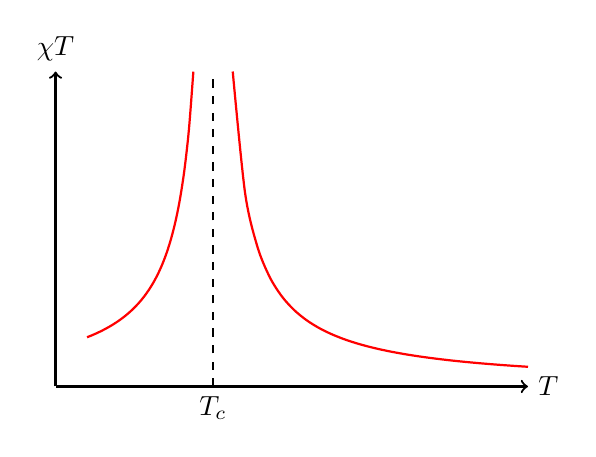
\begin{tikzpicture}
    \pgfmathsetmacro{\axissize}{4};
    \pgfmathsetmacro{\plotsize}{3};
    \pgfmathsetmacro{\tc}{2};
    \draw[thick, ->] (0,0) -- (+6,0) node[right]{$T$};
    \draw[thick, ->] (0, 0) -- (0,+4) node[above]{$\chi\br{T}$};
    \draw[thick, scale=1.0,domain=0.25:4,smooth,variable=\T,red] plot ({\T+\tc},{1/(\T)});
    \draw[thick, scale=1.0,domain=-1.6:-0.25,smooth,variable=\T,red] plot ({\T+\tc},{-1/(\T)});
    \draw[thick, dashed] (\tc, 0) node[below]{$T_c$} -- (\tc, \axissize);
\end{tikzpicture}
\end{center}

The values of critical exponents from our mean-field theory approach are wrong in the sense that they do not correspond to something physical.
In general, critical exponents depend on,
\begin{enumerate}
    \item Nature of order parameter
    \item Symmetry
    \item Dimensionality of the sample
\end{enumerate}
In the language of this more general Landau theory, the mean-field theory approach does not accurately describe the above dependence. First notice that when we first hypothesized \cref{eq:landau_theory_first} we assumed that $\ve M$ was a constant vector that was independent of spatial coordinates (i.e. position in the material). There was no good reason as to why we assumed this and in general we had to have $\ve M\br{\ve r}$ dependent on $\ve r$. In this case the free energy $F$ would be the functional,
\[ F \stackrel{?}{=} \int \dif^3 r \bs{a \br{\ve M \cdot \ve M} + \f{b}{2} \br{\ve M \cdot \ve M}^4} \]
The `$?$' above the equals sign is present because this form for $F$ does not capture any ordering structure among the spins.
If we re-examine the Heisenberg model,
\[ H = - \f{\s J}{2}\sum_{\ba{ij}} \ve S_i \cdot \ve S_j = - \f{\s J}{4} \sum_{\ba{ij}} \bs{\br{\ve S_i - \ve S_j}^2 - \ve S_i^2 - \ve S_j^2} \]
One can see that the $\ve S_i^2,\ve S_j^2$ are independent of the order or structure of the spin locations but $\ve S_i - \ve S_j$ approximates a spin gradient,
\[ \br{\ve S_i - \ve S_j}^2 \sim \vdel \ve S \cdot \vdel \ve S = \br{\vdel M^x}^2 + \br{\vdel M^y}^2+ \br{\vdel M^z}^2 \]
Therefore the free-energy should penalize non-uniformity in $\ve M$,
\[ F = \int \dif^3 r \bs{a \br{\ve M \cdot \ve M} + \f{b}{2} \br{\ve M \cdot \ve M}^4 + \f{1}{2}\rho \vdel \ve M \cdot \vdel \ve M} \eq \label{eq:improve_landau}\]
Where $\rho >0$ is some unknown positive constant. This forms the starting point for an \textit{improved} Landau theory. Calculating critical exponents under the above theory is complicated. Even if we could calculate critical exponents using \cref{eq:improve_landau}, this would still be an incomplete theory for ferro-magnetism. \Cref{eq:improve_landau} still implies that any material at sufficiently low temperatures $T<T_c$ would become a ferromagnet. However not all materials become ferromagnets in this way. The failure of \cref{eq:improve_landau} is that is still does not encapsulate the idea that the electrons which carry the spins (elementary magnetic moments). Therefore we need to take into account the itinerant character of the electrons. The model that accomplishes this is called the \term{Hubbard model}. The kinetic energy terms of the Hubbard model are,
\[ H\tsb{kin} = - t \sum_{\ba{ij}\si} \br{\ket{i \si}\bra{j\si} + \ket{j \si}\bra{i \si}}  \eq\label{eq:hubbard_model_kin}\]
where $t$ is now the usual tunneling constant of an electron traveling through a material (as we invoked frequently in \cref{sec:structure_topological}). Additionally we need to characterize the long-range interactions between spins. This however if too difficult so we approximate the interactions to only be short range. Simplifying for one orbital per atom,
\[ H\tsb{int} = U \sum_{i} n_{i \uu}n_{i \dd} \eq\label{eq:hubbard_model_int}\]
with $n_{i, \si}$ denotes the number operator for the number of atoms localized to atom $i$ with spin $\si$. Terms of the form $n_{i \uu}n_{i \uu}$ are not present due to the Pauli exclusion principle. The Hubbard model is simply \cref{eq:hubbard_model_kin} combined with \cref{eq:hubbard_model_int},
\[ H = - t \sum_{\ba{ij}\si} \br{\ket{i \si}\bra{j\si} + \ket{j \si}\bra{i \si}} + U \sum_{i} n_{i \uu}n_{i \dd} \eq \label{eq:hubbard_ham} \]
Even this extremely simple model cannot be solved exactly (doing so would certainly yield a Nobel prize in physics). We perform mean-field theory approximations in $n_{i,\si}$,
\[ n_{i\si} = \ba{n_{i\si}} + n_{i\si} - \ba{n_{i\si}} \]
Therefore,
\[ n_{i \uu}n_{i\dd} = \br{\ba{n_{i\uu}} + n_{i\uu} - \ba{n_{i\uu}}} \br{\ba{n_{i\dd}} + n_{i\dd} - \ba{n_{i\dd}}} \]
\[ n_{i \uu}n_{i\dd} = \br{n_{i\uu} - \ba{n_{i\uu}}}\br{n_{i\dd} - \ba{n_{i\dd}}} + n_{i \uu} \ba{n_{i \dd}} + n_{i \dd}\ba{n_{i \uu}} + \ba{n_{i \uu}}\ba{n_{i \dd}} - 2\ba{n_{i \uu}}\ba{n_{i \dd}} \]
Once again we assume that the fluctuations are small,
\[ n_{i \uu}n_{i\dd} = n_{i \uu} \ba{n_{i \dd}} + n_{i \dd}\ba{n_{i \uu}} - \ba{n_{i \uu}}\ba{n_{i \dd}} \]
Now we let $n$ denote the average number of electrons per atom (here we assume that this number is uniform $n_i = n$),
\[ n = \ba{n_{i \uu}} + \ba{n_{i \dd}} \]
We define the \term{degree of spin polarization} $\xi$ such that,
\[ \xi \defined \f{\ba{n_{i \uu}} - \ba{n_{i \dd}}}{\ba{n_{i \uu}} + \ba{n_{i \dd}}} \]
\[ \ba{n_{i\uu}} = n \br{\f{1 + \xi}{2}} \qquad \ba{n_{i\dd}} = n \br{\f{1 - \xi}{2}} \eq \label{eq:nupdowndefined} \]
Where $\xi_i = \xi$ is uniform as well for simplicity. Now we have \cref{eq:hubbard_ham} taking the following form,
\[ H = -t \sum_{\ba{ij}\si}\br{\ket{i \si}\bra{j \si} + \ket{j \si}\bra{i \si}} + \f{Un}{2} \sum_{i} \br{n_{i \uu} + n_{i \dd}} - \f{Un\xi}{2} \sum_{i} \br{n_{i \uu} - n_{i \dd}} - \f{Un^2}{4} \br{1 - \xi^2} N \eq \label{eq:hubbard_ham_working_1}\]
Performing a Fourier transform on the lattice site basis states $\ket{i \si}$,
\[ \ket{i \si} = \f{1}{\sqrt{N}} \sum_{k} \ket{k \si} \braket{k \si}{i \si} = \f{1}{\sqrt{N}} \sum_{k} \ket{k \si} e^{- i \ve k \cdot \ve R_i} \]
We obtain the usual localization energies,
\[ \vep_k = - 2 t \sum_{\ve a} \cos \br{\ve k \cdot \ve a} \]
Such that \cref{eq:hubbard_ham_working_1} becomes,
\[ H = \sum_{k,\si} \vep_k \ket{k \si}\bra{k \si} + \f{Un}{2} \sum_{i} \br{n_{i \uu} + n_{i \dd}} - \f{Un\xi}{2} \sum_{i} \br{n_{i \uu} - n_{i \dd}} - \f{Un^2}{4} \br{1 - \xi^2} N \eq \label{eq:hubbard_ham_working_2}\]
The second term of \cref{eq:hubbard_ham_working_2} is a constant (it simply adds up all of the electrons which is presumed constant). Therefore we can neglect this term by absorbing it into the definition of $H$. Splitting the third term into a sum over spin up states and spin down states yields,
\[ H = \sum_{k} \br{\vep_k - \f{Un \xi}{2}} \ket{k \uu}\bra{k \uu} + \sum_{k} \br{\vep_k + \f{Un \xi}{2}} \ket{k \dd}\bra{k \dd} - \f{Un^2}{4} \br{1 - \xi^2} N \eq \label{eq:hubbard_ham_working_3}\]
The physics behind the appearance (or lack of appearance) of magnetism in this model is the comparison between the energy cost of polarization and the interaction energy gain. In order to find the interaction energy gain (average per state),
\[ \f{\ba{H\tsb{int}}}{N} = - \f{U n \xi}{2} \f{1}{N} \sum_{i} \br{\ba{n_{i \uu}} - \ba{n_{i \dd}}} + \f{U n^2 \xi^2}{4} = -\f{U n^2 \xi^2}{2} + \f{U n^2 \xi^2}{4} = -\f{U n^2 \xi^2}{4} \]
The fact that this interaction energy gain is negative means that the system gains (lowers) its energy due to spin polarization. Now let us calculate the kinetic energy cost. There is a kinetic energy cost because we have to fill the $\uu$ and $\dd$ spin states to two different energies. Pursuant to \cref{eq:hubbard_ham_working_3} define this two energies as $\vep_{k \uu}, \vep_{k \dd}$
\[ \vep_{k \uu} = \vep_k - \f{U n \xi}{2} \qquad \vep_{k \dd} = \vep_k + \f{U n \xi}{2} \]
For a given Fermi energy $\vep_F$ we can define two effective Fermi energies for either the spin $\uu$ or spin $\dd$ states.
\[ \vep_{k \uu} - \vep_F = \vep_k - \f{U n \xi}{2} - \vep_F \defined \vep_k - \vep_{F\uu} \qquad \vep_{k \dd} - \vep_F = \vep_k + \f{U n \xi}{2} - \vep_F \defined \vep_k - \vep_{F\dd} \]
Where $\vep_{F\uu}, \vep_{F\dd}$ are defined as follows,
\[ \vep_{F \uu} = \vep_F + \f{U n \xi}{2} \qquad \vep_{F \dd} = \vep_F - \f{U n \xi}{2} \]
Therefore the effective Fermi-energy for the spin $\uu$ ($\dd$) states is raised (lowered). Therefore the expected occupation for the $\uu$ states is equal to half the total $\f{n}{2}$ plus an extra amount given in terms of the density of states $g\br{\vep}$,
\[ \ba{n_{\uu}} = \f{n}{2} + \int_{\vep_F}^{\vep_{F\uu}} \dif \vep g\br{\vep} \approx \f{n}{2} + g\br{\vep_F} \br{\vep_{F\uu} - \vep_{F}} \eq \label{eq:expected_up}\]
Where we approximate $\vep_{F\uu} \approx \vep_{F}$ such that the integral is linearized. Analogously for $n_{\dd}$ we have,
\[ \ba{n_{\dd}} = \f{n}{2} - \int_{\vep_{F\dd}}^{\vep_{F}} \dif \vep g\br{\vep} \approx \f{n}{2} - g\br{\vep_F} \br{\vep_{F} - \vep_{F\dd}} \eq \label{eq:expected_down} \]
Therefore $\ba{n_{\uu}} - \ba{n_{\dd}}$ is the difference of \cref{eq:expected_up} and \cref{eq:expected_down},
\[ \ba{n_{\uu}} - \ba{n_{\dd}} = g\br{\vep_F} \br{\vep_{F\uu} - \vep_{F}} + g\br{\vep_F} \br{\vep_{F} - \vep_{F\dd}} = g\br{\vep_F} \br{\vep_{F\uu} - \vep_{F\dd}} = 2 g\br{\vep_F}\br{\vep_{F\uu} - \vep_{F}} \]
Additionally using \cref{eq:nupdowndefined} and our earlier assumption of occupation uniformity yields,
\[ \ba{n_{\uu}} - \ba{n_{\dd}} = n \xi \]
Therefore combining these two results yields,
\[ \vep_{F\uu} - \vep_{F} = \f{n \xi}{2 g\br{\vep_F}} \]
Then the kinetic energy cost of spin polarization is given by,
\[ E\tsb{kin} = \int_{\vep_F}^{\vep_{F \uu}}\dif \vep \br{\vep g\br{\vep}} - \int_{\vep_{F \dd}}^{\vep_{F}}\dif \vep \br{\vep g\br{\vep}} \]
\begin{align*}
E\tsb{kin}
&\simeq \f{g\br{\vep_F}}{2} \br{\vep_{F \uu}^2 - \vep_{F}^2 - \vep_{F}^{2} + \vep_{F \dd}^2}\\
&= \f{g\br{\vep_F}}{2} \bs{\br{\vep_{F \uu} - \vep_{F}}\br{\vep_{F \uu} + \vep_{F}} + \br{\vep_{F \dd} - \vep_{F}}\br{\vep_{F \dd} + \vep_{F}}}\\
&= \f{g\br{\vep_F}}{2} \br{\vep_{F\uu} - \vep_F} \bs{\br{\vep_{F \uu} + \vep_{F}} - \br{\vep_{F \dd} + \vep_{F}}}\\
&= \f{g\br{\vep_F}}{2} \br{\vep_{F\uu} - \vep_F} \bs{\br{\vep_{F \uu} - \vep_{F}} - \br{\vep_{F \dd} - \vep_{F}}}\\
&= g\br{\vep_F} \br{\vep_{F\uu} - \vep_F}^2 \\
&= \f{n^2 \xi^2}{4 g\br{\vep_F}}
\end{align*}
Therefore the kinetic energy cost is positive. In total, the energy cost is,
\[ E\tsb{tot} = E\tsb{kin} + E\tsb{int} = \f{n^2 \xi^2}{4 g\br{\vep_F}} - \f{U n^2 \xi^2}{4} = \f{n^2 \xi^2}{4 g\br{\vep_F}} \br{1 - U g\br{\vep_F}} \]
Therefore the interaction energy gain dominates the kinetic energy cost when the term in brackets is negative or when,
\[ U g\br{\vep_F} > 1 \]
This inequality is known as the \term{Stoner criterion} named after Edmund Clifton Stoner. The Stoner criterion explains the importance of d-orbitals. In d-orbitals, $g\br{\vep_F}$ is larger because d-orbitals give rise to more narrow bands. Moreover $U$ is larger since d-electrons are more strongly localized (the Coulomb interaction is stronger).

\subsection{Mott Insulators and Anti-Ferromagnetism}
Returning to the Hubbard model,
\[ H = -t \sum_{\ba{ij}\si} \br{\ket{i \si} \bra{j \si} + \ket{j \si} \bra{i \si}} + U \sum_{i} n_{i \uu} n_{i \dd} \eq \label{eq:mott_hubbard_discussion} \]
Consider a half-filled band where there is one electron per site ($n_{i \uu} = 1$ or $n_{i \dd} = 1$, not both). According to band energy theory, this is a metal. However, for large enough $U$, it becomes energetically unfavorable for electrons to move, since moving through a half-filled energy and always involves doubly occupying some sites ($n_{i \uu} = 1$ and $n_{i \dd} = 1$) which by \cref{eq:mott_hubbard_discussion} costs energy $U$. Therefore at roughly $U \sim zt$ there is transition from metal to insulator, which is called a \term{Mott insulator}. An important question in a Mott insulator is what happens to the spins of the localized electrons? \\

Supposing $U$ is sufficiently high that $U \gg 2t$, therefore we can set $t = 0$ in \cref{eq:mott_hubbard_discussion} and analyze,
\[ H = U \sum_{i} n_{i \uu} n_{i \dd}  \]
The ground state of a Mott insulator is where there is exactly one electron at every site, but the spin can either be $\uu$ or $\dd$. Therefore the ground state is $2^{N}$-fold degenerate. This degeneracy is lifted when $t \neq 0$. The question then becomes, how is this degeneracy lifted? To see how this happens, consider the two-site problem where there are $N = 2$ electrons,
\[ H = - t\sum_{\si} \br{\ket{1\si} \bra{2\si} + \ket{2\si} \bra{1\si}} + U \sum_{i \in \bc{1,2}} n_{i \uu} n_{i \dd} \]
Since there are $2$ electrons ($1$ for each site), there are $4$ single-electron states,
\[ \ket{1 \uu} \quad \ket{1 \dd} \quad \ket{2 \uu} \quad \ket{2 \dd} \]
As discussed before, the wavefunction for $2$ electrons must be anti-symmetric. Therefore there are $6$ possible states of $2$ electrons (the notation $\ket{1\dd, 2\uu}$ reads: on site $1$ there is a spin $\dd$ electron and on site $2$ there is a spin $\uu$ electron),
\begin{align*}
    \ket{1\uu, 1\dd} &= -\ket{1\dd, 1\uu} \\
    \ket{1\uu, 2\uu} &= -\ket{2\uu, 1\uu} \\
    \ket{1\uu, 2\dd} &= -\ket{2\dd, 1\uu} \\
    \ket{1\dd, 2\uu} &= -\ket{2\uu, 1\dd} \\
    \ket{1\dd, 2\dd} &= -\ket{2\dd, 1\dd} \\
    \ket{2\uu, 2\dd} &= -\ket{2\dd, 2\uu}
\end{align*}
Therefore we need to find the matrix representation of $H$ in terms of this basis. The matrix-element of such a representation is only nonzero when there are $2$ electrons on either site $1$ or site $2$ (and not one on each),
\[ \bra{1 \uu, 1 \dd} H\tsb{int} \ket{1 \uu, 1 \dd} = \bra{2 \uu, 2 \dd} H\tsb{int} \ket{2 \uu, 2 \dd} = U \]
The remaining elements are all zero. The kinetic energy term turns $\ket{1 \uu}$ into $\ket{2 \uu}$ and $\ket{1 \dd}$ into $\ket{2 \dd}$ and vice versa. Thus we have,
\begin{align*}
\bra{1 \dd, 2 \uu} H\tsb{kin} \ket{1 \dd, 1 \uu} &= -t \\
\bra{1 \dd, 2 \uu} H\tsb{kin} \ket{1 \uu, 1 \dd} &= t
\end{align*}
Therefore the complete Hamiltonian ($H\tsb{kin} + H\tsb{int}$) can be written as,
\[ H = \begin{pmatrix}
    U & 0 & -t & t & 0 & 0 \\
    0 & 0 & 0 & 0 & 0 & 0 \\
    -t & 0 & 0 & 0 & 0 & -t \\
    t & 0 & 0 & 0 & 0 & t \\
    0 & 0 & 0 & 0 & 0 & 0 \\
    0 & 0 & -t & t & 0 & U \\
\end{pmatrix} \]
Clearly the states $\ket{1 \uu, 2 \uu}$ and $\ket{1 \dd, 2 \dd}$ correspond to the 2nd and 5th rows and columns of this matrix and are decoupled from the other states and have eigenenergy $0$. The remaining Hamiltonian, indexed by states $\ket{1 \uu, 2 \dd}, \ket{1 \uu, 2 \dd}, \ket{1 \dd, 2 \uu}$ and $\ket{2 \uu, 2 \dd}$ (respectively) can be written as a $4 \times 4$ matrix,
\[ H = \begin{pmatrix}
    U & -t & t & 0 \\
    -t & 0 & 0 & -t \\
    t & 0 & 0 & t \\
    0 & -t & t & U \\
\end{pmatrix} \]
Its eigenvalues are,
\[ E_1 = 0 \qquad E_2 = U \qquad E_3 = \f12 \br{U + \sqrt{U^2 + 16t^2}} \qquad E_4 = \f12 \br{U - \sqrt{U^2 + 16t^2}} \]
The ground states of the system correspond to the lowest energy eigenvalues. Clearly this is $E_4$,
\[ E_g = E_4 = \f12 \br{U - \sqrt{U^2 + 16t^2}} \]
The corresponding (unnormalized) eigenvector is,
\[ \ket{z} = \br{1, \f{U + \sqrt{U^2 + 16t^2}}{4t}, -\f{U + \sqrt{U^2 + 16t^2}}{4t}, 1} \]
Specifically for Mott insulators we are interested in the case where $U \gg t$. In this case,
\[ \ket{z} \approx \br{0, \f{U}{2t}, -\f{U}{2t}, 0} \]
This ground state wavefunction is,
\[ \ket{\psi} = \f{1}{\sqrt{2}} \br{\ket{1\uu, 2 \dd} - \ket{1 \dd, 2 \uu}} \]
Where $\ket{\psi}$ corresponded to a total spin of $\ve S = 0$ and a ground state energy of,
\[ E_g = \f12 \br{U - \sqrt{U^2 + 16t^2}} \approx \f12 \br{U - U\br{1 + 8\f{t^2}{U^2}}} = - \f{4t^2}{U} \]
Therefore $\s J = \f{4 t^2}{U}$. Using the two spin model $H = \s J \ve S_1 \cdot \ve S_2$ we can immediately generalize to $N$ interacting spin systems where the spin terms are restricted to nearest neighbor interactions,
\[ H = \f{\s J}{2} \sum_{\ba{ij}} \ve S_i \cdot \ve S_j \]
Which is a good description of an anti-ferromagnet because anti-ferromagnets are Mott insulators.
\begin{enumerate}
    \item Ferromagnetism arises from lowering of the interaction energy between the electrons, when the spins are aligned. Ferromagnets are metals. (e.g. Fe, Co, Ni, Mn)
    \item Anti-Ferromagnetism arises from lowering of kinetic energy when spins are anti-aligned. Anti-Ferromagnets are Mott insulators. (e.g. MnO, NiO, La$_2$CnO$_4$)
\end{enumerate}
In is important to understand the qualitative differences between ferromagnets and anti-ferromagnets given their similar models:\\
\textbf{Ferromagnets:}
For ferromagnets our interacting model (with two spins) is,
\[ H = - \s J \ve S_1 \cdot \ve S_2 \]
Where the spins become aligned or anti-aligned in the ground state,
\[ \ket{\psi} \in \bc{\ket{\uu, \uu}, \ket{\dd, \dd}} \]
Where the components of the spin $\ve S = \f{\hbar}{2} \ve \si$ can be written as,
\[ \ve S_1 \cdot \ve S_2 = S_1^xS_1^x + S_1^yS_1^y + S_1^zS_1^z = \f12 \br{S_1^+ S_2^- + S_1^- S_2^+} + S_1^z S_2^z \]
Therefore we see that,
\begin{align*}
    S^z \ket{\uu} &= \f{\hbar}{2}\si^{z}\ket{\uu} = \f{\hbar}{2}\ket{\uu} \\
    S^z \ket{\dd} &= \f{\hbar}{2}\si^{z}\ket{\dd} = \f{\hbar}{2}\ket{\dd} \\
    S^+ \ket{\uu} &= \f{\hbar}{2}\si^{+}\ket{\uu} = \f{\hbar}{2} \begin{pmatrix}
        0 & 2 \\
        0 & 0 \\
    \end{pmatrix}\begin{pmatrix}
        1 \\ 0
    \end{pmatrix}  = 0 \\
    S^- \ket{\uu} &= \f{\hbar}{2}\si^{+}\ket{\uu} = \f{\hbar}{2} \begin{pmatrix}
        0 & 0 \\
        2 & 0 \\
    \end{pmatrix}\begin{pmatrix}
        1 \\ 0
    \end{pmatrix} = \hbar \ket{\dd} \\
    S^+ \ket{\dd} &= \f{\hbar}{2}\si^{+}\ket{\dd} = \f{\hbar}{2} \begin{pmatrix}
        0 & 2 \\
        0 & 0 \\
    \end{pmatrix}\begin{pmatrix}
        0 \\ 1
    \end{pmatrix}  = \hbar \ket{\uu} \\
    S^- \ket{\dd} &= \f{\hbar}{2}\si^{+}\ket{\dd} = \f{\hbar}{2} \begin{pmatrix}
        0 & 0 \\
        2 & 0 \\
    \end{pmatrix}\begin{pmatrix}
        0 \\ 1
    \end{pmatrix} = 0
\end{align*}
Therefore $\ket{\uu, \uu}$ is an eigenstate of $H$ with eigenenergy $- \s J \hbar^2 / 4$,
\[ H \ket{\psi} = -\f{\s J \hbar^2}{4}\bs{\si_1^{z}\si_2^{z} + \f12 \br{\si_1^+ \si_2^- + \si_1^- \si_2^+}} \ket{\uu, \uu} = - \f{\s J \hbar^2}{4}\ket{\uu, \uu} \]
This analysis seems trivial, but becomes illuminating when we consider the analogy for anti-ferromagnets.
\textbf{Ferromagnets:}
For anti-ferromagnets our interacting model (with two spins) is,
\[ H = + \s J \ve S_1 \cdot \ve S_2 \]
A simple guess for the ground state would reasonably be $\ket{\uu, \dd}$ (or $\ket{\dd, \uu}$). This however does not work,
\[ H \ket{\psi} = \f{\s J \hbar^2}{4}\bs{\si_1^{z}\si_2^{z} + \f12 \br{\si_1^+ \si_2^- + \si_1^- \si_2^+}} \ket{\uu, \dd} \not \propto \ket{\uu, \dd} \]
Therefore $\ket{\uu, \dd}$ is \textit{not} the ground state of for anti-ferromagnets. This state, and the analogous multi-spin state, where neighboring spin states have opposite spin, is called the \term{Neel state}.
\begin{center}
    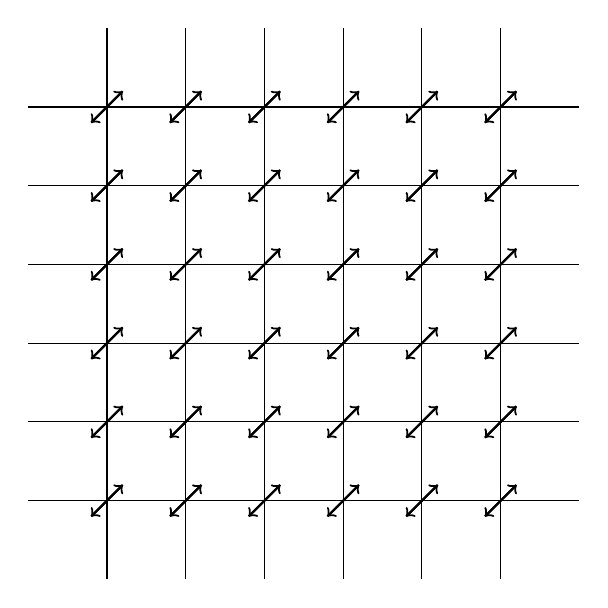
\begin{tikzpicture}
    \pgfmathsetmacro{\spinsize}{0.2}
    \foreach \i in {0,...,5}{
        \draw[thin] (\i, 0-1) -- (\i, 5+1);
    }
    \foreach \j in {0,...,5}{
        \draw[thin] (0-1, \j) -- (5+1, \j);
    }
    \foreach \i in {0,...,5}{
    \foreach \j in {0,...,5}{
        \pgfmathparse{\i+\j}
        \ifthenelse{\isodd{\pgfmathresult}}
        {
            \draw[thick,->] (\i-\spinsize, \j-\spinsize) -- (\i+\spinsize, \j+\spinsize);
        }{
            \draw[thick,<-] (\i-\spinsize, \j-\spinsize) -- (\i+\spinsize, \j+\spinsize);
        }
    }
    }
    \end{tikzpicture}
\end{center}

\section{Superconductivity}
\subsection{Ginzburg-Landau Free Energy}
Most metallic elements (except ferromagnets) and even some non-metals undergo a transition into a superconducting state as the temperature is lowered. Superconductivity is the phenomena where resistivity suddenly drops to zero below a critical temperature $T_c$,

\begin{center}
\begin{tikzpicture}
    \pgfmathsetmacro{\axissize}{4};
    \pgfmathsetmacro{\plotsize}{3};
    \draw[->] (0,0) -- (+\axissize,0) node[right]{$T$};
    \draw[->] (0, 0) -- (0,+\axissize) node[above]{$\rho\br{T}$};
    \draw[scale=1.0,thick, domain=1:\plotsize,smooth,variable=\T,red] plot ({\T},{\plotsize*exp(\T)/exp(\plotsize)});
    \draw[red, thick] (1,0) node[below]{$T_c$} -- (1,{0.1 + 1/\plotsize});
\end{tikzpicture}
\end{center}

A related feature is that that specific heat $C_v$ of the material jumps at the critical temperature as well from $C_v \sim T$ to $C_v \sim e^{-\f{\De}{k_B T}}$. \\
\begin{center}
\begin{tikzpicture}
    \pgfmathsetmacro{\axissize}{4};
    \pgfmathsetmacro{\plotsize}{3};
    \draw[->] (0,0) -- (+\axissize,0) node[right]{$T$};
    \draw[->] (0, 0) -- (0,+\axissize) node[above]{$C_v\br{T}$};
    \draw[scale=1.0,thick, domain=0:1,smooth,variable=\T,red] plot ({\T},{-1 + exp(\T)});
    \draw[red, thick, dashed] (1,0) node[below]{$T_c$} -- (1,{-1+ exp(1)});
    \draw[scale=1.0,thick, domain=1:\plotsize,smooth,variable=\T,red] plot ({\T},{\T});
\end{tikzpicture}
\end{center}

There are two possible ways one could interpret the features of superconductivity. The first is that superconductors are simply ideal metals in which below $T_c$ the electrons do not experience scattering. Alternatively, it could be that a superconductor is a new state of matter. If was the \term{Meissner effect} in the 1930s involving liquefied Helium that first demonstrated the latter; superconductivity is genuinely a new state of matter. In an ideal metal with $\rho = 0$ when $T < T_c$
if we were to start from $T > T_c$ we have $\vdel \times \ve E = - \f1c \pder{\ve B}{t}$. When $T < T_c$ we have that $\pder{\ve B}{t} = 0$ (for an ideal metal). Therefore $\be E = \rho \ve j \implies \ve E = \ve 0$ inside the sample when $T < T_c$. This is fundamentally different than a superconductor which expels all magnetic fields below $T_c$.
\begin{itemize}
    \item Ideal metal: $T < T_c$, $\rho = 0$, $\ve B = \text{const}$
    \item Superconductor: $T < T_c$, $\rho = 0$, $\ve B = \ve 0$
\end{itemize}
Typical superconductors like Al, Sn, Hg have very low critical temperatures ($T_c \sim \SI{1}{\K} - \SI{10}{\K}$) which are non-ideal for use in practical electronics. High temperature super conductors like La$_{2-x}$Sr$_{x}$CnO$_4$ have $T_c \sim \SI{34}{\K}$. The current record holder is HgBa$_2$Ca$_2$CN$_3$O$_8$ with $T_c \sim \SI{133}{\K}$. \\

Microscopically, superconductivity originates from the pairing of electrons. In metallic superconductors this is due to the exchange of phonons: electrons moving through the crystal lattice, polarizes the crystal lattice locally, which attracts another electron. In cuprate high-$T_c$ superconductors, pairing is thought to be due to the anti-ferromagnetic spin-spin interaction of the parent (undoped) Mott insulator. \\

The most important qualitative properties of superconductors can be described using semi-phenomenological \term{Landau-Ginzburg theory}.\\

Pairs of electrons form bosonic states and are considered bosons. Bosons are not constrained by the Pauli exclusion principle; any number of bosons may occupy the ground state. Therefore at zero or low temperatures, all the bosons will want to \textit{condense} into the lowest energy state; the state with zero momentum. In this state, all of the bosons are essentially described by a single wavefunction $\vp\br{\ve r}$. Landau and Ginzburg realized that one may think of $\vp\br{\ve r}$ as an order parameter, just like magnetization in a ferromagnet. Near $T_c$ we may then write down a Taylor expansion of the free energy $F$ in powers of $\vp$. Since the free energy should not depend on the phase of $\vp\br{\ve r}$, it may only depend on $\abs{\vp}^2, \abs{\vp}^4, \ldots$ and so on. Thus,
\[ F = F_0 + V a \abs{\vp}^2 + \f12 V b \abs{\vp}^4 + \cdots \]
Where $F_0$ is the free energy of the normal metallic state which we will omit henceforth. $V$ is the total volume. The ground state occurs when $F$ is minimized,
\[ \f{1}{V} \pder{F}{\abs{\vp}} = 2 a \abs{\vp} + 2 b \abs{\vp}^3 = 0 \]
Therefore we have a ground state,
\[ \abs{\vp} = \sqrt{- \f{a}{b}} \]
Which is possible when $a < 0$ ($b > 0$ always) when $T < T_c$. Therefore,
\[ a \sim \f{T - T_c}{T_c} \]
Therefore,
\[ \abs{\vp} \sim \sqrt{T_c - T} \sim \br{-t}^{\be} \qquad \be = \f12 \]
To describe properties of superconductors it turns out to be very important to describe situations when $\vp\br{\ve r}$ is not uniform. In this case we need to add extra terms to the free energy which depend on the non-uniformity of $\vp\br{\ve r}$; specifically $\vdel \vp\br{\ve r}$. Naively, the following should work by symmetry,
\[ F = \kappa \intl \dif^3 r \abs{\vdel \vp}^2 \]
Where $\kappa > 0$. However, it does not really work since this violates a very important physical principle: {gauge invariance}. When we talked about electrons in a magnetic field, we saw that the momentum operator in a magnetic field was,
\[ \hat p = - i \hbar \vdel  + \f{e}{c} \ve A \]
which was a result of demanding gauge invariance. Consider a wavefunction $\psi\br{\ve r}$. Let us multiply it by an arbitrary position-dependent phase factor $\s X\br{\ve r}$.
\[ \psi\br{\ve r} \mapsto e^{i \s X \br{\ve r}}\psi\br{\ve r} \]
Acting on this new wave-function with the momentum operator yields,
\[ \br{- i \hbar \vdel  + \f{e}{c} \ve A} \br{e^{i \s X \br{\ve r}}\psi\br{\ve r}} = e^{i \s X \br{\ve r}} \bs{- i \hbar \vdel  + \f{e}{c} \ve A + \hbar \vdel \s X} \psi\br{\ve r} \]
Now recall that $\ve A$ is defined only up to a gradient $\ve A \mapsto \ve A + \vdel f$, thus we can make use of the following gauge transformation of $\ve A$,
\[ \ve A \mapsto \ve A - \f{\hbar c}{e} \vdel \s X \]
and obtain,
\[ \br{- i \hbar \vdel  + \f{e}{c} \ve A} \br{e^{i \s X \br{\ve r}}\psi\br{\ve r}} = e^{i \s X \br{\ve r}} \bs{- i \hbar \vdel  + \f{e}{c} \ve A} \psi\br{\ve r} \]
This means that the Schrodinger equation for a particle of charge $-e$ in an electromagnetic field is invariant under the following transformation,
\[ \psi \mapsto e^{i \s X} \psi \qquad \ve A \mapsto \ve A - \f{\hbar c}{e} \vdel \s X \]
In our case, $\vp\br{\ve r}$ is a wave-function of particles with charge $-2e$ (one for each electron). Thus the free energy must be invariant under the following,
\[ \vp \mapsto e^{i \s X} \vp \qquad \ve A \mapsto \ve A - \f{\hbar c}{2e} \vdel \s X \]
This means that the free energy must have the following form,
\[ F = \int \dif^3 r \bs{\f{1}{2 m^*} \abs{\br{-i \hbar \vdel  + \f{e^{*}}{c} \ve A}\vp}^2 + a \abs{\vp}^2 + \f{b}{2}\abs{\vp}^4 + \f{\abs{\ve B}^2}{8\pi} - \f{\ve B \cdot \ve H}{4\pi}} \eq \label{eq:ginzburg-landau}\]
Where $e^* = 2e$ and $m^* = 2m$ and $\ve H$ is an external magnetic field. \Cref{eq:ginzburg-landau} is called the \term{Ginzburg-Landau free energy} of a superconductor. \\

The thermodynamic equilibrium of a state of a superconductor is determined by minimizing $F$ with respect to $\vp$. Determining the equilibrium points requires some variational calculus. Varying $F$ with respect to $\vp^*\br{\ve r}$,
\begin{align*}
    \de_{\vp^*} F
    &= \int \dif \ve r \bs{a \phi \de \vp^* + b \vp \abs{\vp}^2 \de\vp^* + \f{1}{2m^{*}} \br{i\hbar \vdel \de \vp^* + \f{e^*}{c}\ve A \de \vp*}\cdot\br{-i\hbar \vdel \vp + \f{e^*}{c}\ve A \vp}} \eq \label{eq:glfe_variation}
\end{align*}
Consider the first term in the product expansion,
\begin{align*}
    &\int \dif \ve r \vdel \de \vp^* \cdot \br{-i\hbar \vdel + \f{e^*}{c}\ve A}\vp\\
    &\qquad = - \int \dif \ve r \de \vp^* \vdel \cdot \br{-i\hbar \vdel + \f{e^*}{c}\ve A}\vp + \int \dif \ve r \vdel \cdot \bs{\de \vp^* \br{-i\hbar \vdel + \f{e^*}{c}\ve A} \vp} \\
    &\qquad = - \int \dif \ve r \de \vp^* \vdel \cdot \br{-i\hbar \vdel + \f{e^*}{c}\ve A}\vp + \oint \de \vp^* \br{-i\hbar \vdel\vp + \f{e^*}{c}\ve A\vp}\cdot \dif \ve S
\end{align*}
Here $S$ is the surface of the sample. It is possible to neglect the surface term since it only determines the boundary conditions for $\vp$ in a finite sample (i.e. $\de \varphi^*|_S = 0$). Therefore \cref{eq:glfe_variation} becomes,
\begin{align*}
    \de_{\vp^*} F
    &= \int \dif \ve r \bs{a \vp + b \vp \abs{\vp}^2 + \f{1}{2m^*}\br{-i\hbar \vdel + \f{e^*}{c}\ve A}^2 \vp} \de \vp^* = 0
\end{align*}
The thermodynamic equilibrium occurs when $\de_{\vp^*} F = 0$. $\de_{\vp^*} F$ can only equal zero if the expression in the square brackets vanishes at every point in $\ve r$ (this is due to the Raymond-Dubois lemma). Thus we obtain the \term{first Ginzburg-Landau equation}.
\[ \f{1}{2m^{*}}\br{-i\hbar \vdel + \f{e^*}{c} \ve A}^2 \vp + a \vp + b \abs{\vp}^2\vp = 0 \eq \label{eq:first_ginzburg-landau}\]
\Cref{eq:first_ginzburg-landau} looks like a Schrodinger equation for a particle in a magnetic field, but it is clearly non-linear in $\vp$. Note however, that the magnetic field $\ve B = \vdel \times \ve A$ inside the sample is also a thermodynamic variable and we must also vary $F$ with respect to $\ve A$ analogous to how we varied $F$ with respect to $\vp^*$ in \cref{eq:glfe_variation}.
\begin{align*}
    \de_{\ve A} F
    &= \int \dif \ve r \bigg[\f{1}{2m^*} \f{e^*}{c} \de \ve A \vp^* \cdot \br{-i\hbar \vdel + \f{e^*}{c}\ve A}\vp + \f{1}{2m^*}\br{i\hbar\vdel + \f{e^*}{c}\ve A}\vp^* \cdot \f{e^*}{c}\de \ve A \vp + \cdots \\
    &\qquad \cdots +\f{1}{4\pi}\br{\vdel \times \ve A}\cdot \br{\vdel \times \de \ve A} - \f{\ve H}{4\pi}\cdot \br{\vdel \times \de \ve A} \bigg]
\end{align*}
Consider the last two terms, we make use of the following identity: $\ve a \cdot \br{\vdel \times \ve b} = \ve b \cdot \br{\vdel \times \ve a} - \vdel \cdot \br{\ve a \times \ve b}$,
\begin{align*}
    \f{1}{4\pi} \int \dif \ve r \bs{\br{\vdel \times \ve A} - \ve H}\cdot \br{\vdel \times \de \ve A}
    = \f{1}{4\pi}\int \dif \ve r \de \ve A \cdot \vdel \times\br{\vdel \times \ve A} - \f{1}{4\pi} \oint \dif \ve S \cdot \bs{\de \ve A \times \br{\vdel \times \ve A - \ve H}}
\end{align*}
The surface integral vanishes because the magnetic field at the surface of the conductor is fixed by boundary conditions. Thus $\de \ve A|_{S} = \ve 0$. Thus we obtain,
\begin{align*}
    \de_{\ve A} F = \int \dif \ve r \bs{\f{-i\hbar e^*}{2 m^* c}\br{\vp^* \vdel \vp - \vp \vdel \vp^*} + \f{{e^*}^2}{m^* c^2} \abs{\vp}^2 \ve A + \f{1}{4\pi} \vdel \times \br{\vdel \times \ve A}}\cdot \de \ve A = 0
\end{align*}
Setting the integrand to be zero and using the fact that $\vdel \times \br{\vdel \times \ve A} = \vdel \times \ve B = \f{4\pi}{c}\ve j$ we obtain an expression for $\ve j$,
\[ \ve j = \f{i\hbar e^*}{2m^*}\br{\vp^* \vdel \vp - \vp \vdel \vp^*} - \f{{e^*}^2}{m^* c}\abs{\vp}^2\ve A \eq \label{eq:second_ginzburg-landau} \]
This is referred to as the \term{second Ginzburg-Landau equation}. We will now analyze the consequences of \cref{eq:first_ginzburg-landau,eq:second_ginzburg-landau}. We begin by assuming that $T < T_c$ so that we are in the superconducting state. If we assume that $\vp$ is uniform throughout the material, then \cref{eq:first_ginzburg-landau} becomes,
\[ a \vp + b \abs{\vp}^2 \vp = 0 \]
Therefore we have obtained a non-trivial solution to \cref{eq:first_ginzburg-landau},
\[ \abs{\vp} = \sqrt{\f{\abs{a}}{b}} \]
If we interpret $\vp\br{\ve r}$ as the wavefunction of the pair condensate, then $\abs{\vp}^2$ should have the meaning of the number density of pairs in the material,
\[ \abs{\vp}^2 = n_s^* \]
Letting $\vp\br{\ve r} = \sqrt{n_s^*} e^{i \te \br{\ve r}}$, then in a superconducting sample, we can expect $n_s^*$ to be uniform and only $\te\br{\ve r}$ to be depending on $\ve r$. Calculating the current via \cref{eq:second_ginzburg-landau} and we obtain,
\[ \ve j = -\f{\hbar e^* n_s^*}{m^*}\br{\vdel \te + \f{e^*}{\hbar c} \ve A} \]
Therefore the superconducting current $\ve j$ is directly related to the gradient of the phase of the macroscopic condensate wavefunction $\vdel \te \br{\ve r}$. This explains both the Meissner effect and the effect of zero resistance. First consider the Meissner effect. It is possible to remove the phase by a gauge transformation ($\ve A \mapsto \ve A - \f{\hbar c}{e^*} \vdel \te$),
\[ \ve j = - \f{{e^*}^2n_s^*}{m^* c} \ve A \eq \label{eq:j_proper_gauge}\]
Then take the curl of both sides of \cref{eq:j_proper_gauge}. If $\vdel \times \ve B = \f{4\pi}{c}\ve j$,
\[ \vdel \times \br{\vdel \times \ve B} = \f{4\pi}{c}\br{\vdel \times \ve j} = \vdel \br{\vdel \cdot \ve B} - \del^2 \ve B = - \del^2 \ve B \]
\[ \vdel \times \ve j = -\f{{e^*}^2n_s^*}{m^* c}\vdel \times \ve A =  -\f{{e^*}^2n_s^*}{m^* c}\ve B\]
Thus we obtain the following equation for $\ve B$,
\[ \del^2 \ve B = \f{4\pi{e^*}^2n_s^*}{m^*c^2} \ve B = \f{1}{\la^2}\ve B \eq \label{eq:laplace_B}\]
Where $\la$ can be interpreted as the penetration depth of the magnetic field into the superconductor,
\[ \la = \sqrt{\f{m^* c^2}{4 \pi {e^*}^2 n_s^*}} \eq \label{eq:penetration_depth}\]
If, for example, we place the magnetic field parallel to the superconductor with surface normal co-linear to the $\hat x$-axis,
\begin{center}
    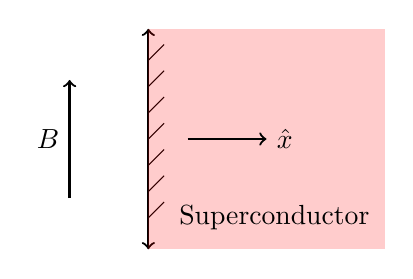
\begin{tikzpicture}
        \draw[thick, <->] (+0, +1.4) -- (+0, -1.4);
        \draw[thick, ->] (-1, -0.75) -- (-1, +0.75) node[midway, left]{$\ve B$};
        \foreach \i in {-3,...,3}{
            \draw (+0,+\i/3) -- ++ (0.2, 0.2);
        }
        \path[fill=red, fill opacity=0.2] (+0, +1.4) -- (+0, -1.4) -- (+3, -1.4) -- (+3, +1.4) -- cycle;
        \draw (+1.6, -1) node[]{Superconductor};
        \draw[thick, ->] (+0.5, +0) -- ++ (+1, +0) node[right]{$\hat x$};
    \end{tikzpicture}
\end{center}
then \cref{eq:laplace_B} determines that $\ve B$ only penetrates a distance of $\la$ into the superconductor,
\[ \dder{B}{x} = \f{1}{\la^2}B \implies B\br{x} = B\br{0}e^{-x/\la} \]
In simple, metallic superconductors, $\la \sim \SI{100}{\angstrom}$ which is much shorter than the characteristic size of the superconducting object. This gives the effect that the magnetic field is expelled from the superconductor and explains that \cref{eq:laplace_B} is the origin of the Meissner effect. \\

\subsection{Persistent Currents}
What about the effect of virtually zero resistivity and \term{persistent currents} in superconducting materials? This can be accomplished by setting up gradients of the phase $\te \br{\ve r}$ inside a superconducting ring.
\begin{center}
    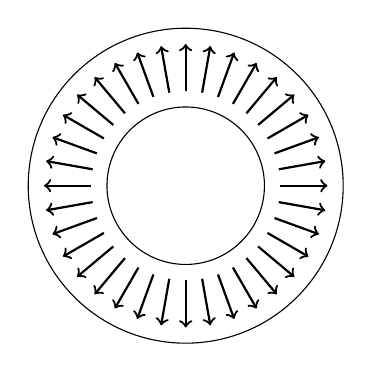
\begin{tikzpicture}
        \draw (0,0) circle (2);
        \draw (0,0) circle (1);
        \foreach \i in {0,...,35} {
            \draw[thick, ->] ({1.2*cos(\i/36*360)}, {1.2*sin(\i/36*360)}) -- ({1.8*cos(\i/36*360)}, {1.8*sin(\i/36*360)});
        }
    \end{tikzpicture}
\end{center}
If we recall some important terms of \cref{eq:ginzburg-landau},
\[ F = \int \dif^3 r \f{\hbar^2 {n_s^*}^2}{2 m^*} \br{\vdel \te + \f{e^*}{\hbar c} \ve A}^2 + \cdots \]
In order to minimize $F$, we roughly want the following to hold inside the ring.
\[ \vdel \te = -\f{e^*}{\hbar c}\ve A\]
This implies that the current must flow at the edge of the ring creating the corresponding magnetic flux,
\[ \ve j = \f{c}{4\pi} \vdel \times \ve B \]
and therefore we must have,
\[ \oint \vdel \te \cdot \dif \ve \ell = 2 \pi n \]
Where $n$ is some integer. Going from the $n=1$ to $n=0$ state requires \textit{unwinding} the phase, which costs a huge amount of energy. The above also implies the quantization of magnetic flux inside the superconducting ring.
\[ \oint \vdel \te \cdot \dif \ve \ell = 2 \pi n = - \f{e^*}{\hbar c}\oint \vdel A \cdot \dif \ve \ell = - \f{e^*}{\hbar c} \vp \]
Thus the magnetic field is quantized in units of $\vp_0$,
\[ \vp_0 = \f{hc}{e^*} = \f{hc}{2e} \]
and a measurement of magnetic flux quantization proves that electrons pairing in superconductors is a valid model.

\subsection{Type I \& Type II Superconductors}
One important length scale for a superconductor is the penetration depth $\la$ of the magnetic field (\cref{eq:penetration_depth}) derived above via \cref{eq:laplace_B}.
\[ \la = \sqrt{\f{m^* c^2}{4 \pi {e^*}^2 n_s^*}} \]
There is another length scale, the coherence length $\xi$, which is related to how the superconducting order parameter $\vp\br{\ve r}$ varies spatially. Consider the first Ginzburg-Landau equation \cref{eq:first_ginzburg-landau},
\[ \f{1}{2m^{*}}\br{-i\hbar \vdel + \f{e^*}{c} \ve A}^2 \vp + a \vp + b \abs{\vp}^2\vp = 0 \]
Suppose there was no magnetic field $\ve A = \ve 0$ and look for a solution that satisfies the following boundary conditions,
\[ \vp\br{x = 0} = 0 \qquad \vp\br{x \to \inf} = \sqrt{-\f{a}{b}} \eq \label{eq:normal_sc_bc}\]
This solution represents a boundary between a normal and superconducting material,
\[ - \f{\hbar^2}{2m^*}\dder{\vp}{x} + a \vp + b \abs{\vp}^2 \vp = 0 \eq \label{eq:normal_sc_equation}\]
The solution to \cref{eq:normal_sc_equation} that satisfies the relevant boundary conditions \cref{eq:normal_sc_bc} is,
\[ \varphi\br{x} = \sqrt{-\f{a}{b}} \tanh\br{\f{x}{\sqrt{2}\xi}} \]
Where $\xi$ is the \term{coherence length},
\[ \xi = \sqrt{\f{\hbar^2}{-2 m^* a}} \]
The coherence length $\xi$ determines the extent to which the superconducting wavefunction will penetrate into the region associated with the normal material. The ratio of $\la$ and $\xi$, $\s X = \la / \xi$ is an important parameter. Superconductors with $\s X < 1/\sqrt{2}$ are called \term{type I superconductors}, while $\s X>1/\sqrt{2}$ are \term{type II superconductors}. \\

Consider a superconductor in a magnetic field. When the field is expelled, the free energy density is given by,
\[ f = a \abs{\vp}^2 + \f{b}{2}\abs{\vp}^4 \]
The non-trivial solution occurs at $\abs{\vp}^2 = - \f{a}{b}$ which means that the free energy density becomes,
\[ f = - \f{a^2}{b} + \f{a^2}{2 b} = -\f{a^2}{2b} \]
Which is referred to as the \term{condensation energy}. The system gains condensation energy by transitioning into the superconducting state. However, magnetic energy is lost when the field is expelled from the superconductor:
\[ f_m = \f{B^2}{8\pi} - \f{BH}{4\pi} = - \f{H^2}{8 \pi} \]
When the magnetic field is large enough, the loss of magnetic energy will become larger than the gain in condensation energy and the superconductor will be destroyed and will allow the field to penetrate. This happens at the thermodynamic critical field $H_c$,
\[ \f{H_c^2}{8\pi} = \f{a^2}{2b} \implies H_c = \sqrt{\f{4 \pi a^2}{b}} \]
At this critical magnetic field, $a \sim T - T_c$ which implies $H_c \sim \abs{T - T_c}$.
\begin{center}
    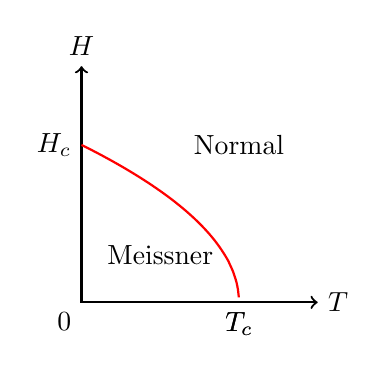
\begin{tikzpicture}
        \draw[thick,<->] (3, 0) node[right]{$T$} -- (0,0) node[below left]{$0$} -- (0, 3) node[above]{$H$};
        % \draw[thick] (0,2) arc (90:0:2);
        \draw[thick] (2, 0) node[below]{$T_c$};
        \draw[thick] (0, 2) node[left]{$H_c$};
        \draw[thick] (2, 0) node[below]{$T_c$};
        \draw[thick] (1,0.6) node[]{Meissner};
        \draw[thick] (2,2) node[]{Normal};
        \draw[thick, scale=1.0,domain=0:2,samples=200,variable=\x,red] plot ({\x},{2*((2-\x)^(0.5))/((2)^(0.5))});
    \end{tikzpicture}
\end{center}
Additionally the magnetic susceptibility $\chi$ produces perfect diamagnetism,
\[ B = H + 4 \pi M = 0 \implies H = - 4 \pi M \implies \chi = \pder{M}{H} = -\f{1}{4\pi} \]
\begin{center}
    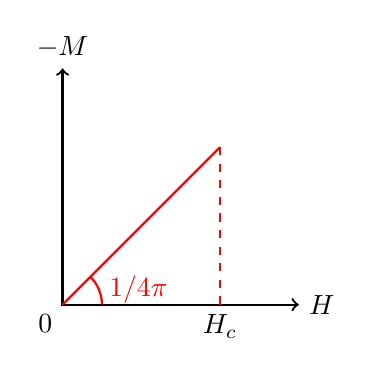
\begin{tikzpicture}
        \draw[thick,<->] (3, 0) node[right]{$H$} -- (0,0) node[below left]{$0$} -- (0, 3) node[above]{$-M$};
        \draw[thick, red] (0.5,0) arc (0:45:0.5) node[midway, right]{$1/4\pi$};
        \draw[thick] (2, 0) node[below]{$H_c$};
        % \draw[thick] (0, 2) node[left]{$\f12$};
        \draw[thick, red] (0,0) -- (2,2);
        \draw[thick, red, dashed] (2,0) -- (2,2);
    \end{tikzpicture}
\end{center}
In reality, this only holds true for type I superconductors. \\

Suppose we have constructed a large field $H$, much greater than $H_c$, and begin decreasing the field strength. We can expect the superconducting state to appear when the first Ginzburg-Landau equation (\cref{eq:first_ginzburg-landau}) has non-trivial solution. The field, at which this happens, is different from $H_c$, and is called ${H_c}_2$. Near ${H_c}_2$ we can expect $\abs{\vp}$ to be small, enabling us to neglect the non-linear term in \cref{eq:first_ginzburg-landau}. In this regime, we have,
\[ \f{1}{2m^*}\br{-i\hbar \vdel + \f{e^*}{c} \ve A}^2 \vp = - a \vp \]
This is simply the Schrodinger equation for a charged particle in a magnetic field with energy $-a$. If we choose the Landau gauge $\ve A = x B \hat y$, then \cref{eq:first_ginzburg-landau} becomes,
\[ - \f{\hbar^2}{2m^*}\br{\pdder{}{x} + \pdder{}{z}} \vp + \f{1}{2m^*}\br{-i\hbar \pder{}{y} + \f{e^*}{c} B x}^2 \vp = - a \vp \]
Conjecturing an ansatz of the following form $\vp\br{\ve r} = e^{i\br{k_y y + k_z z}} \phi\br{x}$, we obtain the auxiliary equation,
\[ -\f{\hbar^2}{2m^*}\dder{\phi}{x} + \br{\f{e^*B}{c}}^2 x^2 \phi + \f{\hbar k_y e^* B}{c}x \phi = \br{-a - \f{\hbar^2k_y^2}{2m^*}- \f{\hbar^2k_z^2}{2m^*}} \phi\]
This is simply a Schrodinger equation for a harmonic oscillator with the minimum of the potential energy shifted from $x = 0$ to $x = x_0 = - k_y \ell^2$ where have defined the usual \term{magnetic length},
\[ \ell = \sqrt{\f{\hbar c}{e^* B}} \]
Completing the square we obtain,
\[ - \f{\hbar^2}{m^*}\dder{\phi}{x} + \f{m^* \w_c^2}{2}\br{x - x_0}^2 \phi = E \phi \]
Where we have the defined the following constants,
\[ E = - a - \f{\hbar^2 k_z^2}{2m^*} \qquad \w_c = \f{e^* B}{m^* c} \]
The eigenenergies of this Schrodinger equation will have the following form,
\[ E_n = \hbar \w_c \br{n + \f12} \]
For this equation to have a solution, we must have $E = E_n$ for some $n \in \bc{1,2,\ldots}$. The largest value of $B$ for which a solution exists is found from,
\[ E_0 = \f{\hbar \w_c}{2} = E\br{k_z = 0} = -a \implies \f{\hbar e^* B\tsb{max}}{2m^* c} = - a \implies B\tsb{max} = {H_c}_2 = - \f{2am^*c}{\hbar e^*}\]
${H_c}_2$ can be expressed in terms of $\s X$ and $H_c$,
\[ {H_c}_2 = - \f{2am^*c}{\hbar e^*} = \f{H_c}{-a \sqrt{\f{4\pi}{b}}} = \sqrt{2}\f{m^* c}{\hbar e^*} \sqrt{\f{b}{2\pi}} H_c \]
Using $n_s = \abs{\vp}^2 = - \f{a}{b}$,
\[ \s X = \f{\la}{\xi} = \sqrt{\f{m^* c^2}{4 \pi {e^*}^2 n_s}} \cdot \sqrt{\f{- 2 m^* a}{\hbar^2}} = \sqrt{\f{m^* c^2 b}{4 \pi {e^*}^2 \br{-a}}} \cdot \sqrt{\f{- 2 m^* a}{\hbar^2}} = \f{m^* c}{\hbar e^*} \sqrt{\f{b}{2\pi}} \]
Thus we obtain,
\[ {H_c}_2 = \sqrt{2}\s X H_c \]
Which justifies the different behaviour of type I and II superconductors. When $\s X > 1 / \sqrt{2}$ we have ${H_c}_2 > H_c$.
\begin{center}
    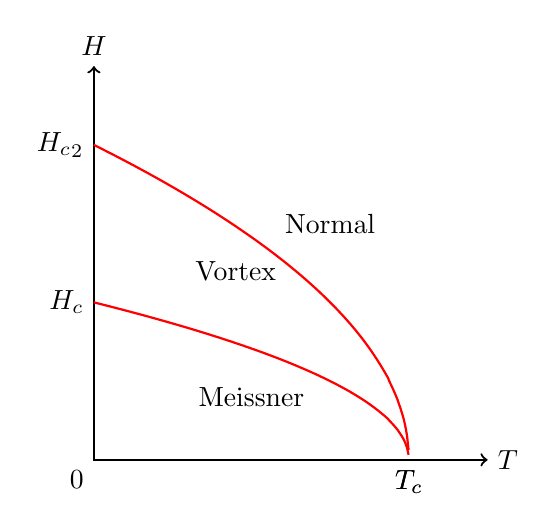
\begin{tikzpicture}[scale=2]
        \draw[thick,<->] (2.5, 0) node[right]{$T$} -- (0,0) node[below left]{$0$} -- (0, 2.5) node[above]{$H$};
        % \draw[thick] (0,2) arc (90:0:2);
        \draw[thick] (2, 0) node[below]{$T_c$};
        \draw[thick] (0, 2) node[left]{${H_c}_2$};
        \draw[thick] (0, 1) node[left]{${H_c}$};
        \draw[thick] (2, 0) node[below]{$T_c$};
        \draw[thick] (1,0.4) node[]{Meissner};
        \draw[thick] (0.9,1.2) node[]{Vortex};
        \draw[thick] (1.5,1.5) node[]{Normal};
        \draw[thick, scale=1.0,domain=0:2,samples=200,variable=\x,red] plot ({\x},{1*((2-\x)^(0.5))/((2)^(0.5))});
        \draw[thick, scale=1.0,domain=0:2,samples=200,variable=\x,red] plot ({\x},{2*((2-\x)^(0.5))/((2)^(0.5))});
    \end{tikzpicture}
\end{center}
In type II superconductors, there exists a superconducting state at fields $H > H_c$. In this state the field penetrates inside the superconductor, yet $\abs{\vp}$ is still non-zero and the sample is superconducting.
\[ {H_c}_2 = -\f{2a m^* c}{\hbar e^*} = - \f{2m^* a}{\hbar^2} \f{\hbar c}{e^*} = \f{\varphi_0}{2 \pi \xi^2} \]
Where $\varphi_0 = h c /e^*$ is the flux quantum. Thus ${H_c}_2$ corresponds to one flux quantum per area $2 \pi \xi^2$.

\subsection{Josephson Effects}
Let us imagine we have two pieces of a superconducting material that are initially detached from each other and each are described by their own wavefunctions $\phi_1\br{\ve r}, \phi_2\br{\ve r}$.
\begin{center}
    \begin{tikzpicture}
        \draw (-2,+0) node[draw, minimum width=3em, minimum height=3em]{$\phi_1\br{\ve r}$};
        \draw (+2,+0) node[draw, minimum width=3em, minimum height=3em]{$\phi_2\br{\ve r}$};
    \end{tikzpicture}
\end{center}

Furthermore assume that $\abs{\phi_1} = \abs{\phi_2} = \sqrt{n_s}$ (i.e. the two wavefunctions have the same norm but might having differing phases that are spatially dependent).
\[ \phi_1\br{\ve r} = \sqrt{n_s} e^{i\te_1\br{\ve r}} \qquad \phi_2\br{\ve r} = \sqrt{n_s} e^{i\te_2\br{\ve r}} \]
Afterwards, suppose we bring the two materials together such that they become adjacent. It is possible to model this composite system simply by considering the tunneling between the two regions with amplitude $t$,
\begin{center}
    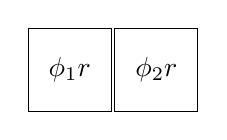
\begin{tikzpicture}
        \draw (-0.55,+0) node[draw, minimum width=3em, minimum height=3em]{$\phi_1\br{\ve r}$};
        \draw (+0.55,+0) node[draw, minimum width=3em, minimum height=3em]{$\phi_2\br{\ve r}$};
    \end{tikzpicture}
\end{center}
Electrons in the first material $\ket{1}$ can tunnel to the second material $\ket{2}$ and vice versa via the following Hamiltonian,
\[ H = - t \br{\ket 1 \bra 2 + \ket 2 \bra 1} = \begin{pmatrix}
    0 & -t \\ -t & 0
\end{pmatrix} \]
The composite wavefunction at the interface is $\phi\br{\ve r} = \f{1}{\sqrt{2}} \br{\phi_1\br{\ve r} + \phi_2\br{\ve r}}$ whose dynamics is modeled by the Schrodinger equation $H\phi = E \phi$. Because of $\phi$, we have the following \term{supercurrent},
\[ \ve j = \f{i \hbar e^{*}}{2m^{*}} \br{\phi^{*} \vdel \phi - \phi \vdel \phi^*} \]
Computing the gradient would be difficult in general because the phases $\te_1, \te_2$ are position dependent. Instead, we can liberally approximate the gradient across the interface as,
\[ \vdel \phi \approx \f{\phi_2 - \phi_1}{L} \hat x \]
Where $L$ is the characteristic length of the interface in the $\hat x$-direction. Then we have,
\begin{align*}
    \phi^* \vdel \phi - \phi \vdel \phi^*
    &\propto \br{\phi_1^* + \phi_2^*}\br{\phi_2 - \phi_1} - \br{\phi_2 + \phi_1} \br{\phi_2^* - \phi_1^*} \\
    &= \phi_1^* \phi_2 - \abs{\phi_1}^2 + \abs{\phi_2}^* - \phi_2^* \phi_1 - \phi_2^* \phi_1 - \abs{\phi_2}^2 + \abs{\phi_1}^* + \phi_1^* \phi_2 \\
    &= 2\br{\phi_1^* \phi_2 - \phi_2^* \phi_1} \\
    &= 2n_s \br{e^{-i\te_1}e^{i\te_2} - e^{i\te_1}e^{-i\te_2}} \\
    &= -4 i n_s \sin \te \qquad \te \defined \te_1 - \te_2
\end{align*}
This supercurrent is present even in the absence of a external electric field. If the two adjacent materials are superconductors, this current always flows across the junction on the absence of voltage. This current where $I = I_c \sin \te$ is called the \term{DC-Josephson effect/current}.\\

Instead if we subject the two materials to an external potential $V$,
\begin{center}
    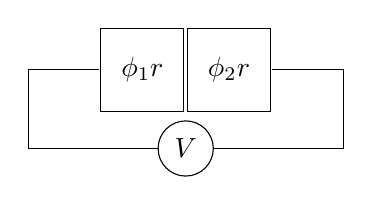
\begin{tikzpicture}
        \draw (-0.55,+0) node[draw, minimum width=3em, minimum height=3em]{$\phi_1\br{\ve r}$};
        \draw (+0.55,+0) node[draw, minimum width=3em, minimum height=3em]{$\phi_2\br{\ve r}$};
        \draw (+0,-1) -- (+2, -1) -- (+2,+0) -- (+1.1, +0);
        \draw (-0,-1) -- (-2, -1) -- (-2,+0) -- (-1.1, +0);
        \draw (0, -1) node[draw, circle, fill=white, ]{$V$};
    \end{tikzpicture}
\end{center}

Then the system Hamiltonian becomes,
\[ H = \begin{pmatrix}
    e V & - t \\
    -t & - e V
\end{pmatrix} \eq \label{eq:ACJC_H} \]
Where the dynamics of $\phi$ are governed by the Schrodinger equation $i \hbar \pder{\phi}{t} = H \phi$ which is explicitly,
\begin{align*}
\eq\label{eq:ACJC}
\begin{split}
    i\hbar \pder{\phi_1}{t} &= e V \phi_1 - t \phi_2 \\
    i\hbar \pder{\phi_2}{t} &= - t \phi_1 - e V \phi_2
\end{split}
\end{align*}
Instead of solving this set of equations directly, we can make use of the conjugate forms of \cref{eq:ACJC},
\begin{align*}
\eq\label{eq:ACJC_conj}
\begin{split}
    -i\hbar \pder{\phi_1^*}{t} &= e V \phi_1^* - t \phi_2^* \\
    -i\hbar \pder{\phi_2^*}{t} &= - t \phi_1^* - e V \phi_2^*
\end{split}
\end{align*}
Multiplying \cref{eq:ACJC,eq:ACJC_conj} by factors of $\phi_1, \phi_2$, we can sum the results and reconstruct the supercurrent,
\[ i\hbar \br{\phi_2^* \phi_1 - \phi_1^* \phi_2} = i \hbar \br{\phi_1 \pder{\phi_2^*}{t} + \phi_2^* \pder{\phi_1}{t} - \phi_2 \pder{\phi_1^*}{t} - \phi_1^* \pder{\phi_2}{t}}\]
Substituting \cref{eq:ACJC},
\begin{align*}
    i\hbar \br{\phi_2^* \phi_1 - \phi_1^* \phi_2}
    &= eV \phi_2^* \phi_1 - t \abs{\phi_2}^2 + e V \phi_2^* \phi_1 + t \abs{\phi_1}^2 + eV \phi_1^* \phi_2 - t \abs{\phi_1}^2 + e V \phi_1^* \phi_2 + t \abs{\phi_2}^2 \\
    &= 2 e V \br{\phi_2^* \phi_1 - \phi_1^* \phi_2} \\
    &= 4 e V n_s \cos \te \\
    &= i \hbar \pder{}{t}\br{-2 i n_s \sin \te} \\
    &= 2 \hbar n_s \cos \te \pder{\te}{t}
\end{align*}
Therefore we obtain the \term{Josephson relation} for $\te$,
\[ \pder{\te}{t} = \f{2eV}{\hbar} \]
If $V$ is a constant, i.e. we apply a external DC voltage and the phase response becomes linear in time,
\[ \phi\br{t} = \phi\br{0} + \f{2eV}{\hbar}t \]
The responding current however is oscillatory,
\[ I\br{t} = I_c \sin \bs{\phi\br{0} + \f{2eV}{\hbar}t} \]
This is referred to as the \term{AC-Josephson effect}. It is surprising to see an AC response from the application of a DC external voltage. The fact that the frequency of oscillation depends on the voltage $V$ and fundamental constants $2e/\hbar$, measurements of this frequency represent our most precise measurement of ${e}/{\hbar}$. In combination with the quantum hall effect, which gives a precise measurement of $e^2/\hbar$, we obtain our most precise values for $e$ and $\hbar$, some of the most fundamental physical constants.\\

Analyzing the Josephson effect in this way is incomplete; we have failed incorporate the effects of resistance of the junction. If we subject the junction to a larger current than $I_c$ we will have some residual effects,

\begin{itemize}
    \item $I < I_c$: the current flows without resistance, $\implies V = 0$
    \item $I > I_c$: part of the current will become non-superfluid
\end{itemize}
This is referred to as a \term{resistively shunted Josephson junction}. The total current can be decomposed into the two effects,
\[ I = I_c \sin \te + \f{V}{R} \]
Where $I_c\sin\te$ is the supercurrent through the junction and $\f{V}{R}$ is the dissipative current which is modeled as a current passing through a resistor with resistance $R$.\\

Therefore given that the the time-derivative of the phase $\pder{\te}{t}$ is governed by the external potential $V$,
\[ V = \f{\hbar}{2e} \pder{\te}{t} \eq \label{eq:Vddtphi}\]
We conclude that,
\[ I = I_c \sin \te + \f{\hbar}{2 e R} \der{\te}{t} \]
which is a differential equation for $\te\br{t}$ that can be solved.
\[ \der{\te}{t} = \f{2eR}{\hbar}\br{I - I_c \sin \te} = \f{2 I e R}{\hbar} \br{1 - \f{I_c}{I}\sin \te} \]
Let $\la$ and $\w_{0}$ be the following parameters,
\[ \la \defined \f{I_c}{I} < 1 \qquad \w_0 = \f{2IeR}{\hbar}  \]
Where $\la$ is dimensionless and $\w_0$ as units of frequency. Therefore we obtain the following non-linear differential equation,
\[ \der{\te}{t} = \w_0\br{1 - \la \sin \te} \]
Integrating this separable equation,
\[ \w_0\cdot \br{t - t_0} = \intl \f{\dif \te}{1 - \la \sin \te} \]
Since $\la < 1$ we have that the integrand never diverges and moreover, it can be solved analytically,
\[ \tan \f{\te}{2} = \la + \sqrt{1 - \la^2} \tan\bs{\f12 \sqrt{1 -\la^2} \w_0 \br{t - t_0}} \]
Therefore,
\[ \te\br{t} = 2\tan^{-1}\bc{\la + \sqrt{1 - \la^2} \tan\bs{\f12 \sqrt{1 -\la^2} \w_0 \br{t - t_0}}} \]
Using \cref{eq:Vddtphi} we obtain a time-dependent voltage $V\br{t}$ in response to a DC current,
\[ V\br{t} = R \f{I^2 - I_c^2}{I - I_c \cos \w t} \qquad \w = \f{2e}{\hbar} R \sqrt{I^2 - I_c^2} \]
If instead we are interested in the time averaged voltage $\ba{V}$, we can calculate that as well,
\[ \ba{V} = \f{w}{2\pi}\int_{0}^{\f{2\pi}{\w}} V\br{t}\dif t = \f{\hbar \w}{2e} = R \sqrt{I^2 - I_c^2} \]
\begin{center}
    \begin{tikzpicture}
        \draw[thick, <->] (0, +3) node[above]{$\ba{V}$} -- (0, 0) -- (+3, 0) node[right]{$I$};
        \draw (+1, 0) node[below]{$I_c$};
        \draw[thick,scale=1.0,domain=1:3,samples=200,variable=\I,red] plot ({\I},{sqrt(\I^2 - 1^2)});
        \draw[thick,dashed,scale=1.0,domain=0:3,samples=200,variable=\I,red] plot ({\I},{\I});
    \end{tikzpicture}
\end{center}
Evidently at high current $I$, the junction behaves classically.

\subsection{SQUID - Superconducting Quantum Interference Device}
\begin{center}
    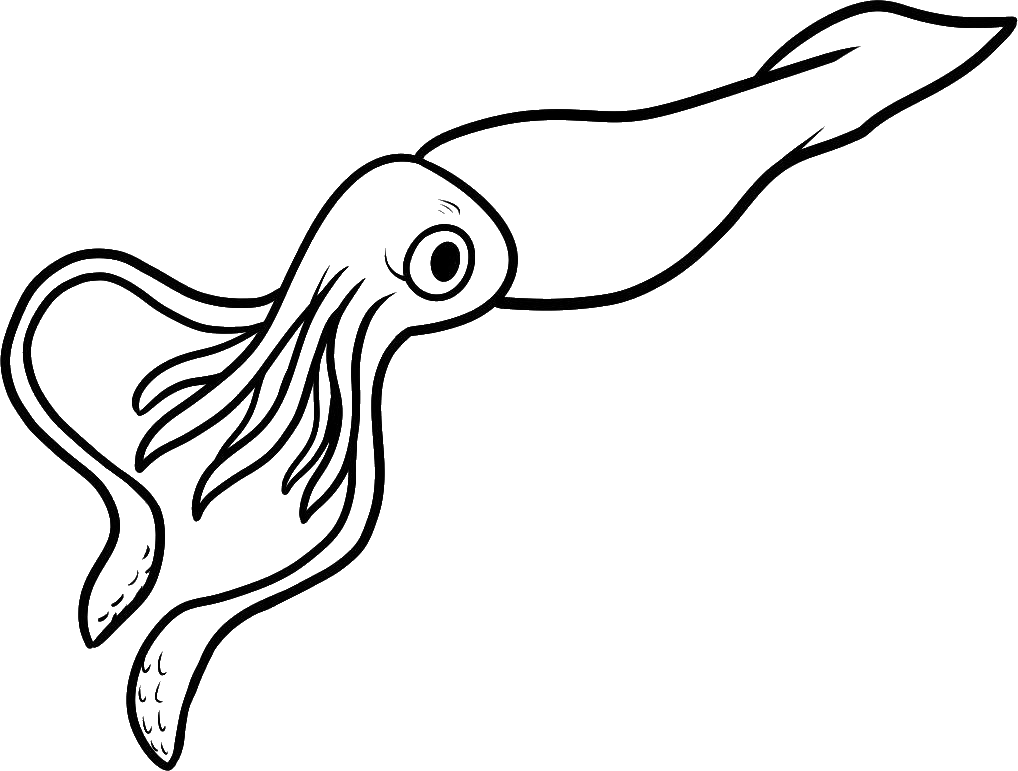
\includegraphics[width=0.6\textwidth]{figures/squid.png}
\end{center}
Suppose we had two Josephson junctions (labeled $a, b$) arranged in the following configuration,
\begin{center}
    \begin{tikzpicture}
        \pgfmathsetmacro{\dd}{0.25};
        \pgfmathsetmacro{\ww}{2};
        \pgfmathsetmacro{\tt}{1};
        \pgfmathsetmacro{\zz}{0.8};
        \draw (-\dd, +3*\tt) -- (-\dd, +2*\tt) -- (-\ww, +2*\tt) -- (-\ww, -2*\tt) -- (-\dd, -2*\tt) -- (-\dd, -3*\tt);
        \draw (+\dd, +3*\tt) -- (+\dd, +2*\tt) -- (+\ww, +2*\tt) -- (+\ww, -2*\tt) -- (+\dd, -2*\tt) -- (+\dd, -3*\tt);
        \draw[scale=0.8] (+\ww, +2*\tt) -- (-\ww, +2*\tt) -- (-\ww, -2*\tt) -- (+\ww, -2*\tt) -- cycle;
        \draw[dashed, scale=0.9] (+\ww, +\zz) node[below]{$3$} -- (+\ww, +2*\tt) -- (-\ww, +2*\tt) -- (-\ww, +\zz) node[below]{$1$};
        \draw[dashed, scale=0.9] (+\ww, -\zz) node[above]{$4$} -- (+\ww, -2*\tt) -- (-\ww, -2*\tt) -- (-\ww, -\zz) node[above]{$2$};
        \draw[->] (+0, +3*\tt) node[above]{$I$} -- ++(0, -1);
        \draw[<-] (+0, -3*\tt) node[below]{$I$} -- ++(0, +1);
        \draw[] (-\ww*0.9, +0) node[draw, fill=black, fill opacity=0.2]{$a$};
        \draw[] (-\ww*0.9, +0) node[]{$a$};
        \draw[] (+\ww*0.9, +0) node[draw, fill=black, fill opacity=0.2]{$b$};
        \draw[] (+\ww*0.9, +0) node[]{$b$};
    \end{tikzpicture}
\end{center}
It is possible to calculate the relative phase differences between the labeled points $1,2,3,4$ by integrating along the dashed paths,
\[ \ve j = - \f{\hbar e^* n_s}{m^*} \br{\vdel \te + \f{e^*}{\hbar c} \ve A} \]
\[ \vdel \te = - \f{e^*}{\hbar c} \ve A \]
\[ \te_3 - \te_1 + \te_2 - \te_4 = -\f{2e}{\hbar c} \oint \ve A \cdot \dif \ve \ell \]
\[ \varphi_a = \te_2 - \te_1 \qquad \varphi_b = \te_4 - \te_3 \]
Therefore the difference of the two phase differences across the two junctions is,
\[ \varphi_a - \varphi_b = -\f{2e}{\hbar c}\phi = - 2\pi \f{\phi}{\phi_0} \qquad \phi_0 \defined \f{hc}{2e}\]
Therefore the currents across the junctions are,
\[ I_a = I_c \sin \varphi_a \qquad I_b = I_c \sin \varphi_b \]
And the total interference becomes,
\[ I = I_a + I_b = I_c \br{\sin \vp_A + \sin \vp_b} = 2 I_c \sin\br{\f{\vp_a + \vp_b}{2}}\cos\br{\f{\vp_a - \vp_b}{2}} \]
Which corresponds to a macroscopic interference between the two junctions. But we also have that,
\[ \vp_b = \vp_a + 2 \pi \f{\phi}{\phi_0} \]
Therefore,
\[ I = 2 I_c \sin\br{\f{\pi\phi}{\phi_0}}\cos\br{\vp_a + \f{\pi \phi}{\phi_0}} \]
The maximal current through the SQUID for a given $\phi$ is therefore,
\[ I\tsb{max} = 2 I_c \abs{\cos \br{\f{\pi \phi}{\phi_0}}} \]
Thus a SQUID device bay be used to measure magnetic flux and can act as very sensitive magnetometer.\\

\subsection{Josephson Junction Qubit}
A Josephson junction already has a two-level behave depending on whether $I > I_c$ or $I < I_c$. We have already consider the effect of the supercurrent $I_c \sin \te$ and the residual ordinary current $\f{V}{R}$ but here is a final term that heretofore we have neglected; namely that the Josephson junction also acts as a capacitor,
\[ I = I_c \sin \te + \f{V}{R} + C \der{V}{t} \eq \label{eq:jjc}\]
Where $V = \f{\hbar}{2e} \der{\te}{t}$ still holds. Therefore \cref{eq:jjc} can be written in terms of $\te$,
\[ I = I_c \sin \te + \f{\hbar}{2eR}\der{\te}{t} + \f{\hbar C}{2e} \dder{\te}{t} \]
\[ \dder{\te}{t} + \f{1}{RC} \der{\te}{t} + \f{2eI_c}{\hbar C} \sin \te = \f{2eI}{\hbar C} \eq \label{eq:jjc_te}\]
Above we considered the over-damped limit of the above equation where $\f{1}{RC}$ is very large and we could neglect the second derivative term. Classically we can interpret $\te$ as the coordinate of a classical particle. Doing so, we can correct assign a physical interpretation to the terms in \cref{eq:jjc_te}. Doing so means that \cref{eq:jjc_te} acts as an equation of motion for a particle in a potential,
\[ U\br{\te} \sim - I \te - I_c \cos \te \]
Which is known as a \term{washboard potential} and can be visualized as a tilted cosine curve,
\begin{center}
    \begin{tikzpicture}
        \draw[thick, <->] (0, +3) node[above]{$U\br{\te}$} -- (0, 0) -- (+5, 0) node[right]{$\te$};
        \draw[thick,scale=1.0,domain=0:5,samples=200,variable=\I,red] plot ({\I},{2-0.3*\I-0.2*cos(deg(3*pi*\I))});
    \end{tikzpicture}
\end{center}
Under this interpretation, the velocity of the particle $\der{\te}{t}$ corresponds to the voltage. This system behaves like a qubit because it can be in one of two states. When $I < I_c$, the particle is trapped in one of the minimum where $\der{\te}{t} = 0 \implies V = 0$. Alternatively if $I > I_c$ then the particle is moving down this potential and its motion gives rise to a finite voltage. For each of the potential wells, there will be a number of quantized energy levels that the particle can have. For sufficiently small junctions, it is possible to create a superposition between the lowest energy states of neighboring wells. This is called a \term{current-biased qubit}. The \textit{tilt} of the washboard potential is adjusted by the applied current and changes the energy difference between the ground state and the first excited states.\\

Another type of qubit is a flux qubit. The free energy of a superconductor is given by \cref{eq:ginzburg-landau},
\[ F = \f{\hbar^2 n_s}{2m^*} \int \dif^3 r \br{\vdel \te + \f{2e}{\hbar c} \ve A}^2 \]
Now suppose we construct a ring as a circle of radius $R$.
\begin{center}
    \begin{tikzpicture}
        \pgfmathsetmacro{\xx}{2};
        \pgfmathsetmacro{\yy}{1};
        \draw[thick] (0,0) circle ({sqrt(\xx^2 + \yy^2)});
        \draw[thick, ->] (0,0) -- node[above]{$R$} (\xx, \yy);
        \draw[thick, ->] (\xx, \yy) -- node[right]{$\hat \te$} ++({-0.5*\yy}, {0.5*\xx});
    \end{tikzpicture}
\end{center}
Such that the magnetic flux is $\phi$,
\[ \ve A = \f{\phi}{2\pi R} \hat \te \qquad \oint \ve A \cdot \dif \ve \ell = \phi\]
Therefore the free energy becomes,
\[ F = \f{\hbar^2 n_s}{2 m^*} \int \dif^3 r \br{\vdel \te + \f{2e}{\hbar c} \f{\phi}{2\pi R}\hat \te}^2 \]
Furthermore since $\hat \te \propto \dif \ve \ell$,
\[ \oint \vdel \te \cdot \dif \ve \ell = 2 \pi n \implies \vdel \te  = \f{n}{R} \hat \te  \]
Therefore,
\begin{align*}
F
&= \f{\hbar^2 n_s}{2 m^*} V \br{\f{n}{R} + \f{2e}{\hbar c} \f{\phi}{2\pi R}}^2 \\
&= \f{\hbar^2 n_s V}{2 m^* R^2} \f{e^2}{\pi^2 \hbar^2 c^2}\br{\phi + n \phi_0}^2
\end{align*}
Defining $\la$ such that,
\[\f{e^2 n_s V}{2 \pi m^* R^2 c^2} = \f{V}{8 \pi^3 \la^2 R^2} \]
Yields,
\[ F\br{\phi} = \f{V}{\br{2\pi}^3 \la^2 R^2} \br{\phi + n \phi_0}^2 \]
Parameterized by the integer $n$ we have the following plot for the free energy,
\begin{center}
    \begin{tikzpicture}
        \draw[thick, <->] (-3, +0) -- (+3, +0) node[right]{$\phi$};
        \draw[thick,  ->] (+0, +0) -- (+0, +4) node[above]{$F\br{\phi}$};
        \draw[thick, <->, scale=1.0,domain=-1:+1,samples=50,variable=\x,red] plot ({\x+2},{3*(\x)^2});
        \draw[thick, <->, scale=1.0,domain=-1:+1,samples=50,variable=\x,red] plot ({\x+1},{3*(\x)^2});
        \draw[thick, <->, scale=1.0,domain=-1:+1,samples=50,variable=\x,red] plot ({\x-0},{3*(\x)^2});
        \draw[thick, <->, scale=1.0,domain=-1:+1,samples=50,variable=\x,red] plot ({\x-1},{3*(\x)^2});
        \draw[thick, <->, scale=1.0,domain=-1:+1,samples=50,variable=\x,red] plot ({\x-2},{3*(\x)^2});
        \draw[thick] (-2, +0.2) -- (-2, -0.2) node[below]{$-2\phi_0$};
        \draw[thick] (-1, +0.2) -- (-1, -0.2) node[below]{$-\phi_0$};
        \draw[thick] (+0, +0.2) -- (+0, -0.2) node[below]{$0$};
        \draw[thick] (+1, +0.2) -- (+1, -0.2) node[below]{$\phi_0$};
        \draw[thick] (+2, +0.2) -- (+2, -0.2) node[below]{$2\phi_0$};
    \end{tikzpicture}
\end{center}
When $\phi = \phi_0/2$, there becomes two degenerate states in the neighboring wells. In this state, we have a two state system, a valid qubit.

\subsection{Abrikosov Vortex Lattice}

Consider the structure of the vortex state in Type II superconductors. Suppose the external field is only \textit{slightly} less than ${H_{c}}_2$. Then the solution of the Ginzburg-Landau equation should be nearby the solutions to the linearized the GL equation:
\[ - \f{\hbar^2}{2 m^*} \dder{\vp}{x} + \f{\w^{*} \w_{c}}{2} \br{x - x_0}^2 \vp = E \vp \]
With $E = - a = \hbar \w_c /2$ and $H = {H_{c}}_{2}$,
\[ {H_{c}}_2 = - \f{2am^{*}c}{\hbar e^{*}} \]
The magnetic length $\ell$ is the usual,
\[ \ell^2 = \f{\hbar c}{e^{*} H} = \f{\hbar c}{e^{*} {H_{c}}_{2}} = \f{\hbar c}{e^{*}}\br{- \f{2am^{*}c}{\hbar e^{*}}}^{-1} = -\f{\hbar^2}{2 a m^{*}} = \xi^2  \]
Another way to understand ${H_{c}}_2$ is to consider that ${H_{c}}_2$ is the magnetic field at which the magnetic length length $\ell$ is equal to the coherence length $\xi$. The solutions of the linearized GL equation with $E = \hbar \w_c / 2$ have the following form up to a normalization constant,
\[ \vp_{k_y}\br{x} = e^{-\f{1}{2\ell^2}\br{x + k_y \ell^2}^2} \]
Since we have $\ell = \xi$,
\[ \vp_{k_y}\br{x} = e^{-\f{1}{2\xi^2}\br{x + k_y \xi^2}^2} \]
These represent the lowest order Landau level wavefunctions which should be familiar from the Integer Quantum Hall Effect. The true solutions for the non-linear GL equation for $H$ slightly less that ${H_{c}}_2$ should be a linear combination of these wavefunctions. The trick is to find the correct combination. Suppose we look for a solution that is uniform in the $z$-direction, i.e. the direction of the magnetic field. Then the lowest Landau level eigenstates have the following form,
\[ \phi_{k_y}\br{\ve r} = e^{ik_y y}e^{-\f{1}{2\xi^2}\br{x + k_y \xi^2}^2} \]
Alexei Alexeyevich Abrikosov's idea was to look for a solution, which is periodic in space. Let $d$ be the spatial period in the $y$-direction. The corresponding reciprocal lattice vectors then become,
\[ G_{n} = Gn = \f{2\pi}{d}n \]
where $n \in \Z$ is any integer. We can reduce the wavevector $k_y$ to the first Brillouin zone $k_{y} \mapsto k_y + Gn$, and look for a solution in the form of Bloch functions,
\[ \phi_k\br{\ve r} = \sum_{n=-\inf}^{\inf} c_n e^{ik_y y + i Gn y}e^{-ik_x\br{k_y \xi^2 + G n \xi^2}} e^{-\f{1}{2 \xi^2} \br{x + k_y \xi^2 + G n \xi^2}^2} \]
Where the appropriate coefficients $c_n$ need to be found. Note that if we take the coefficients $c_n$ to be periodic in $n$, then the solution will also be automatically period in the $x$-direction. Indeed, let $c_{n+m} = c_n$.
\begin{align*}
\phi_k\br{x + G \xi^2 m, y}
&= \sum_{n=-\inf}^{\inf} c_n e^{ik_y y}e^{i Gn y}e^{-ik_x\br{k_y \xi^2 + G n \xi^2}} e^{-\f{1}{2 \xi^2} \br{x + k_y \xi^2 + G n \xi^2 + G m\xi^2}^2} \\
&= \sum_{n=-\inf}^{\inf} c_{n-m} e^{ik_y y}e^{i Gn y}e^{-i Gm y}e^{-ik_x\br{k_y \xi^2 + G n \xi^2}}e^{ik_xGm\xi^2} e^{-\f{1}{2 \xi^2} \br{x + k_y \xi^2 + G n \xi^2}^2} \\
&= e^{-i Gm y}e^{ik_xGm\xi^2}\sum_{n=-\inf}^{\inf} c_{n-m} e^{ik_y y}e^{i Gn y}e^{-ik_x\br{k_y \xi^2 + G n \xi^2}} e^{-\f{1}{2 \xi^2} \br{x + k_y \xi^2 + G n \xi^2}^2} \\
&= e^{-i Gm y}e^{ik_xGm\xi^2}\phi_k\br{x,y}
\end{align*}
Therefore $\phi_k$ becomes periodic in the $x$-direction up to a phase factor. We need to choose the period $m$. The simplest choice, made originally by Abrikosov, is to take $m = 1$. It was latter shown that the lowest energy solution is actually obtained with $m=2$, but this is unimportant here. With $m = 1$, all $C_n = C$ are constant can we obtain,
\[ \phi_k\br{\ve r} = c \sum_{n=-\inf}^{\inf} e^{ik_y y}e^{iGny} e^{-k_x G n\xi^2}e^{-ik_x k_y\xi^2}e^{-\f{1}{2\xi^2}\br{x + k_y\xi^2 + Gn\xi^2}^2} \eq \label{eq:mbf}\]
Since $G\xi^2$ is the period in the $x$-direction, we must have,
\[ G \xi^2 = \f{2\pi}{G} \implies G^2 = \f{2\pi}{\xi^2} \implies d = \sqrt{2\pi \xi^2}, G = \f{\sqrt{2\pi}}{\xi} \]
The functions $\phi_k\br{\ve r}$ are called magnetic Bloch functions. Simplifying \cref{eq:mbf},
\begin{align*}
\phi_k\br{\ve r}
&= c \sum_{n=-\inf}^{\inf} e^{ik_y y}e^{iGny} e^{-k_x G n\xi^2}e^{-ik_x k_y\xi^2}e^{-\f{1}{2\xi^2}\br{x + k_y\xi^2 + Gn\xi^2}^2} \\
&= c e^{ik_y y}e^{-ik_x k_y\xi^2} \sum_{n=-\inf}^{\inf}e^{iGny} e^{-k_x G n\xi^2}e^{-\f{1}{2\xi^2}\br{x + k_y\xi^2 + Gn\xi^2}^2} \\
&= c e^{ik_y y}e^{-ik_x k_y\xi^2} \sum_{n=-\inf}^{\inf}e^{iGny} e^{-k_x G n\xi^2}e^{-\f{1}{2\xi^2}\br{x + k_y\xi^2}^2}e^{-\f{2}{2\xi^2}\br{x + k_y\xi^2}\br{Gn\xi^2}}e^{-\f{1}{2\xi^2}\br{Gn\xi^2}^2} \\
&= c e^{ik_y y}e^{-ik_x k_y\xi^2} \sum_{n=-\inf}^{\inf}e^{in\br{Gy - Gk_x\xi^2 + i G\br{x+k_y\xi^2}}} e^{-\f{G^2\xi^2}{2}n^2}e^{-\f{1}{2\xi^2}\br{x + k_y\xi^2}^2} \\
&= c e^{ik_y y}e^{-ik_x k_y\xi^2}e^{-\f{1}{2\xi^2}\br{x + k_y\xi^2}^2} \sum_{n=-\inf}^{\inf}e^{in\br{Gy - Gk_x\xi^2 + i G\br{x+k_y\xi^2}}} e^{-\f{G^2\xi^2}{2}n^2} \\
&= c e^{ik_y y}e^{-ik_x k_y\xi^2}e^{-\f{1}{2\xi^2}\br{x + k_y\xi^2}^2} \te_{3}\br{\f12\br{y - k_x\xi^2 + i \br{x+k_y\xi^2}}, e^{-\f{G^2 \xi^2}{2}}}
\end{align*}
Where $\te_3\br{z, q}$ is the \term{Jacobi $\te$-function}.
\[ \te_{3}\br{z,q} = \sum_{n=-\inf}^{\inf} q^{n^2} e^{2niz} \]
Where $z,q$ can be re-expressed as,
\[ z = \f{iG}{2}\br{x+k_y \xi^2 - i \br{y - k_x\xi^2}} \]
\[ q = e^{-\f{G^2\xi^2}{2}} = e^{-\pi} \]
The most interesting property of the $\te_3\br{z,q}$ function for us is that its zeros occur at the following points,
\[ z = \bs{m + \f12 + \br{n + \f12}\tau}\pi \]
Where $m,n$ are integers and $q = e^{i\pi \tau}$. In our case $\tau = i$ meaning that,
\[ z = \bs{m + \f12 + i\br{n + \f12}}\pi \]
By equating real and imaginary parts we obtain,
\begin{align*}
\f{G}{2}\br{x + k_y \xi^2} &= \br{n + \f12}\pi \\
\f{G}{2}\br{y - k_x \xi^2} &= \br{m + \f12}\pi
\end{align*}
\begin{align*}
x + k_y \xi^2 &= \f{\pi\br{2n + 1}}{G} \\
y - k_x \xi^2 &= \f{\pi\br{2m + 1}}{G}
\end{align*}
Then we get the following,
\begin{align*}
x &=  - k_y \xi^2 + \f{\pi\br{2n + 1}}{G} = \br{n+\f12}d - k_y \xi^2\\
y &=  + k_x \xi^2 + \f{\pi\br{2m + 1}}{G} = \br{m+\f12}d + k_x \xi^2
\end{align*}
and therefore the zeros can be found at,
\[ \ve r\tsb{zeros} = \br{n+\f12}d \hat x + \br{m+ \f12}d \hat y - \br{\ve k \times \hat z}\xi^2 \]
Thus the zeros form a square lattice with lattice constant $d$. The phase of $\phi_k\br{\ve r}$ winds by $2\pi$ around each zero. These zeros thus represent vortices of the superconducting wavefunction. Returning to $\phi_k\br{\ve r}$, we can find the normalization constant $c$,
\begin{align*}
    \int \dif^2 r \abs{\phi_k \br{\ve r}}^2
    &= \abs{c}^2 \cdot \int\dif x \dif y e^{-\f{1}{\xi^2}\br{x + k_y \xi^2}^2} \sum_{n,m = -\inf}^{\inf} e^{i G\br{n-m}\br{y - k_y \xi^2}}e^{-G\br{n+m}\br{x+ k_y \xi^2}}e^{-\f{G^2\xi^2}{2}\br{n^2+m^2}}
\end{align*}
Recalling that we have the following identity,
\[ \f{1}{L_y} \int_{- \f{L_y}{2}}^{\f{L_y}{2}} \dif y e^{i G \br{n - m} y} = \de_{n,m} \]
We obtain,
\begin{align*}
    \int \dif^2 r \abs{\phi_k \br{\ve r}}^2
    &= \abs{c}^2 L_y \int_{-\inf}^{\inf}\dif x e^{-\f{1}{\xi^2}x^2} \sum_{n = -\inf}^{\inf} e^{-2 G nx - G^2 \xi^2 n^2} \\
    &= \abs{c}^2 L_y \sum_{n = -\inf}^{\inf} \sqrt{\pi}\xi e^{\f{4G^2n^2\xi^2}{4} - G^2\xi^2n^2}
\end{align*}
The sum over $n$ only extends to finite values of $\abs{n}$, such that $Gn \xi^2$ is within the limits of the superconducting sample. This means that $- \f{L_x}{2} \leq G n \xi^2 \leq \f{L_x}{2}$, i.e. there are $L_x / G \xi^2$ allowed values of $n$. Then we obtain,
\[ \abs{c}^2 L_y \sqrt{\pi} \xi \f{L_x}{G \xi^2} = 1 \]
Therefore,
\[ \abs{c}^2 = \f{G \xi}{L_xL_y \sqrt{\pi}} = \f{\sqrt{2\pi}}{L_xL_y \sqrt{\pi}} = \f{\sqrt{2}}{L_x L_y} \]
Thus taking $c$ to be real,
\[  c = \f{2^{1/4}}{\sqrt{L_xL_y}} = \sqrt{\f{\sqrt{2\pi} \xi}{L_x}} \f{1}{\sqrt{\sqrt{\pi} L_y \xi}} \]
Where $\br{\sqrt{\sqrt{\pi} L_y \xi}}^{-1}$ is the coefficient of the lowest Landau level wavefunction in the Landau gauge. Finally,
\[ \phi_k\br{\ve r} = \f{2^{1/4}}{\sqrt{L_xL_y}} e^{- ik_xk_y \xi^2} e^{i k_y y} e^{-\f{1}{2 \xi^2}\br{x + k_y \xi^2}^2} \cdot \te_3\bs{\f{G}{2}\br{y - k_x \xi^2 + i \br{x + k_y \xi^2}}, e^{-\pi}} \]

\end{document}
